%% LyX 2.0.6 created this file.  For more info, see http://www.lyx.org/.
%% Do not edit unless you really know what you are doing.
\documentclass[12pt,oneside,italian]{book}
\usepackage{mathptmx}
\usepackage{helvet}
\usepackage[latin1]{inputenc}
\usepackage[T1]{fontenc}
\usepackage[a4paper]{geometry}

\geometry{verbose,tmargin=3cm,bmargin=3cm,lmargin=3.5cm,rmargin=2.5cm,headheight=2cm,headsep=0.5cm}
\pagestyle{empty}
\setlength{\parskip}{\smallskipamount}
\setlength{\parindent}{0pt}
\usepackage[italian]{babel}    % utilizza la lingua italiana come predefinita
\usepackage{pdfpages}

% Questi pacchetti servono per usare font ams per le formule
\usepackage{amsmath}
\usepackage{amsfonts}
\usepackage{amssymb}
\usepackage{attrib}

\usepackage{setspace}
\doublespacing
\usepackage[unicode=true,pdfusetitle,
 bookmarks=false,
 breaklinks=false,pdfborder={0 0 0},backref=false,colorlinks=false]
 {hyperref}
%\usepackage{breakurl}

\makeatletter

%%%%%%%%%%%%%%%%%%%
% OLD FUNCTION FILE BEGIN
% E' una reimplementazione dell'ambiente verbatim che previene l'overflow
% della memoria per lunghi testi.
\usepackage{verbatim}
\usepackage{alltt}

\usepackage[section]{placeins}
\usepackage{subfig}
\usepackage{float}
\usepackage{tikz}


\usepackage{listings}

\usepackage{url}
\urlstyle{same}


%\usepackage{bera}% optional: just to have a nice mono-spaced font
\usepackage{xcolor}

\colorlet{punct}{red!60!black}
\definecolor{background}{HTML}{EEEEEE}
\definecolor{delim}{RGB}{20,105,176}
\colorlet{numb}{magenta!60!black}

\usepackage[scaled]{beramono}
\newcommand\Small{\fontsize{9}{9.2}\selectfont}
\newcommand*\LSTfont{\Small\ttfamily\SetTracking{encoding=*}{-60}\lsstyle}

\lstdefinelanguage{JSON}{
    basicstyle=\LSTfont,
    %numbers=left,
    numberstyle=\scriptsize,
    stepnumber=1,
    numbersep=8pt,
    showstringspaces=false,
    breaklines=true,
    frame=lines,
    backgroundcolor=\color{background},
    literate=
     *{0}{{{\color{numb}0}}}{1}
      {1}{{{\color{numb}1}}}{1}
      {2}{{{\color{numb}2}}}{1}
      {3}{{{\color{numb}3}}}{1}
      {4}{{{\color{numb}4}}}{1}
      {5}{{{\color{numb}5}}}{1}
      {6}{{{\color{numb}6}}}{1}
      {7}{{{\color{numb}7}}}{1}
      {8}{{{\color{numb}8}}}{1}
      {9}{{{\color{numb}9}}}{1}
      {:}{{{\color{punct}{:}}}}{1}
      {,}{{{\color{punct}{,}}}}{1}
      {\{}{{{\color{delim}{\{}}}}{1}
      {\}}{{{\color{delim}{\}}}}}{1}
      {[}{{{\color{delim}{[}}}}{1}
      {]}{{{\color{delim}{]}}}}{1},
}

\lstdefinelanguage{YAML}[]{XML}{
    basicstyle=\LSTfont,
    %numbers=left,
    numberstyle=\scriptsize,
    stepnumber=1,
    numbersep=8pt,
    showstringspaces=false,
    breaklines=true,
    frame=lines,
    backgroundcolor=\color{background},
    literate=
     *{-}{{{\color{punct}-}}}{1}
      {>}{{{\color{punct}>}}}{1}
      {<}{{{\color{punct}<}}}{1}
      {|}{{{\color{punct}|}}}{1}
      {:}{{{\color{punct}{:}}}}{1}
      {,}{{{\color{punct}{,}}}}{1}
      {[}{{{\color{delim}{[}}}}{1}
      {]}{{{\color{delim}{]}}}}{1},
}
\lstdefinelanguage{MYXML}[]{XML}{
    basicstyle=\LSTfont,
    %numbers=left,
    numberstyle=\scriptsize,
    stepnumber=1,
    numbersep=8pt,
    showstringspaces=false,
    breaklines=true,
    frame=lines,
    backgroundcolor=\color{background},
}

%\lstdefinestyle{sharpc}{language=[Sharp]C, frame=lr, rulecolor=\color{blue!80!black}}

\usepackage{color}
\definecolor{bluekeywords}{rgb}{0.13,0.13,1}
\definecolor{greencomments}{rgb}{0,0.5,0}
\definecolor{redstrings}{rgb}{0.9,0,0}

\lstdefinelanguage{CSharp}
{
  basicstyle=\LSTfont,
  numberstyle=\scriptsize,
  stepnumber=1,
  numbersep=8pt,
  language=[Sharp]C,
  showspaces=false,
  showtabs=false,
  breaklines=true,
  showstringspaces=false,
  breakatwhitespace=true,
  escapeinside={(*@}{@*)},
  commentstyle=\color{greencomments},
  keywordstyle=\color{bluekeywords},
  stringstyle=\color{redstrings},
}

%\lstdefinelanguage{CSharp}
%{
% morecomment = [l]{//}, 
% morecomment = [l]{///},
% morecomment = [s]{/*}{*/},
% morestring=[b]", 
% sensitive = true,
% morekeywords = {abstract,  event,  new,  struct,
%   as,  explicit,  null,  switch,
%   base,  extern,  object,  this,
%   bool,  false,  operator,  throw,
%   break,  finally,  out,  true,
%   byte,  fixed,  override,  try,
%   case,  float,  params,  typeof,
%   catch,  for,  private,  uint,
%   char,  foreach,  protected,  ulong,
%   checked,  goto,  public,  unchecked,
%   class,  if,  readonly,  unsafe,
%   const,  implicit,  ref,  ushort,
%   continue,  in,  return,  using,
%   decimal,  int,  sbyte,  virtual,
%   default,  interface,  sealed,  volatile,
%   delegate,  internal,  short,  void,
%   do,  is,  sizeof,  while,
%   double,  lock,  stackalloc,   
%   else,  long,  static,   
%   enum,  namespace,  string}
%}

% === Integrazione delle figure ===========================
% Il package graphicx permette di inserire figure all'interno dei documetni LaTeX.
% Con l'opzione [draft] vengono visualizzati i soli riquadri delle figure. Questa
% opzione � utile per eseguire una compilazione veloce per verificare il posizionamento
% delle figure. 
\usepackage{graphics}
%\usepackage[draft]{graphicx}
\usepackage{graphicx}

% Con questo comando si dice a LaTex dove sono memorizzate le figure
\graphicspath{{./imgs/}}

% Usare le sottofigure e figure flottanti
%\usepackage{subfigure}


% === Regolazione dei margini =============================
% Si regolano i margini in modo da centrare orizzontalmente il testo nella
% pagina
\usepackage{indentfirst}
%\parindent=1em
\usepackage{microtype}
\frenchspacing
\addtolength{\oddsidemargin}{20pt}
\addtolength{\evensidemargin}{-20pt}

% Consente di definire in modo flessible note e titoli
\usepackage{fancyhdr}

% Permette di creare celle che spaziano su pi� righe
\usepackage{multirow}

%%%%%%%%%%%%%%%%%%%
% OLD FUNCTION FILE END

%%%%%%%%%%%%%%%%%%%%%%%%%%%%%% LyX specific LaTeX commands.
%% A simple dot to overcome graphicx limitations
\newcommand{\lyxdot}{.}


%%%%%%%%%%%%%%%%%%%%%%%%%%%%%% Textclass specific LaTeX commands.
\numberwithin{equation}{section}
\numberwithin{figure}{section}

\@ifundefined{date}{}{\date{}}
%%%%%%%%%%%%%%%%%%%%%%%%%%%%%% User specified LaTeX commands.
% INTESTAZIONI
% -----------------

\usepackage{fancyhdr}
\pagestyle{fancy}
\fancyhead{}
\fancyfoot{}
\cfoot{\thepage}
\chead{
\includegraphics[width=\textwidth]{unitemplate/intestazione.pdf}}


% SFONDO
% ----------

\usepackage{eso-pic,graphicx}
\makeatletter
\newcommand\BackgroundPicture[2]{
\setlength{\unitlength}{1pt}
\put(0,\strip@pt\paperheight){
\parbox[t][\paperheight]{\paperwidth}{
\vfill
\centering\includegraphics[angle=#2]{#1}
\vfill
}
}
}
\makeatother


\usepackage{natbib}

\makeatletter  
\let\@orig@endthebibliography\endthebibliography  
\renewcommand\endthebibliography{%  
\xdef\@kept@last@number{\the\c@enumiv}%  
\@orig@endthebibliography}  
\newenvironment{thesitography}[1]  
{\def\bibname{Siti consultati}% Classe book o report  
% {\def\refname{Siti consultati}% Classe article  
\thebibliography{#1}%  
\setcounter{enumiv}{\@kept@last@number}%  
}  
{\@orig@endthebibliography}  
\makeatother 

\begin{document}


\begin{frontmatter}


\includepdf[pages=-]{unitemplate/frontespizio}

\AddToShipoutPicture{\BackgroundPicture{unitemplate/logo.png}{0}}

\tableofcontents

\listoffigures

\end{frontmatter}



\begin{mainmatter}




%%%%%%%%%%%%%%%%%%%%%%%%%%%%%%%%%%%%%%%%%%%%%%%%%%%%%%%%%%%
% Capitolo 1

\chapter*{Introduzione}
\label{ref:intro}  \addcontentsline{toc}{chapter}{Introduzione}

Introduzione.............

%%%%\clearpage{\pagestyle{empty}\cleardoublepage}
%%%%%%%%%%%%%%%%%%%%%%%%%%%%%%%%%%%%%%%%%%%%%%%%%%%%%%%%%%%
% Capitolo 1

\chapter{Contesto ed obiettivi}
\label{ref:contesto}
In questo capitolo sarà introdotto il contesto in cui ci si trova ad operare e gli obiettivi del progetto.


\section{DATABENC}
Il progetto DATABENC (\url{http://www.databenc.it}) (Distretto Ad Alta Tecnologia per i BENi Culturali) è nato in Campania, grazie all'Università degli Studi di Napoli Federico II e all'Università di Salerno, con l'intento di stabilire una programmazione strategica per valorizzare i beni culturali, il patrimonio ambientale e il turismo.
DATABENC ha l'obiettivo di costituire, tra università, centri di ricerca, imprese e amministrazioni comunali presenti sul territorio, una rete che focalizzi le proprie risorse su di un programma di alta tecnologia al fine di creare nuove realtà imprenditoriali (spin-off e start-up), nuove figure professionali, percorsi di alta formazione qualificati, valorizzazione delle conoscenze (brevetti, know-how). 
Il distretto è un contenitore in cui riunire ed integrare itinerari eterogenei di ricerca, formazione ed innovazione, con l'obiettivo comune della tutela e della valorizzazione del patrimonio culturale campano inteso in senso esteso: territori, siti, beni e attività. 
\subsection{Le linee di intervento}
Gli ambiti di intervento del Distretto si sviluppano su tre linee portanti: 
\begin{itemize}
\item Conoscenza integrata: la prima forma di tutela di un bene è nella conoscenza e, per tale motivo, è necessario realizzare un esauriente sistema di salvaguardia cognitiva del patrimonio culturale;
\item Monitoraggio diagnostico: ai fini della tutela di un bene risulta indispensabile il monitoraggio diagnostico inteso in senso ampio, che non si limiti solo alla verifica dell'integrità materiale del bene stesso ma si estenda anche all'area in cui il bene è inserito o alle dinamiche turistiche che lo coinvolgono;
\item Fruizione sostenibile: un aspetto fondamentale del bene culturale è quello del suo utilizzo.  Perciò risulta indispensabile conseguire un utilizzo sostenibile del patrimonio culturale.
\end{itemize}

In sintesi, DATABENC ha come obiettivo l'introduzione di una nuova ottica con cui affrontare il grave problema della tutela e della valorizzazione del patrimonio culturale, e la creazione di un sistema che faccia della Campania una regione dell'innovazione e un centro di produzione e diffusione di cultura capace di attrarre capitali economici e, soprattutto, capitali umani.


\section{Ancitel}

Ancitel S.p.A. (\url{http://www.ancitel.it}) è la principale società dell'ANCI - Associazione Nazionale Comuni Italiani - e da 25 anni supporta gli enti locali nella gestione di tutti i processi di innovazione.
Dalla sua fondazione, avvenuta nel 1987,  Ancitel affianca le pubbliche amministrazioni locali con un'ampia rete di servizi e progetti ideati per rispondere alle loro esigenze operative quotidiane.
In quanto partner dei Comuni, Ancitel agisce ed opera ogni giorno come centro di competenza per fornire loro soluzioni e strumenti pensati per facilitarne e supportarne l'azione quotidiana ed affrontare le sfide dell'innovazione. 
Grazie ad una profonda conoscenza delle dinamiche interne alla Pubblica Amministrazione, Ancitel ha conseguito notevoli capacità di ascolto, dialogo ed intervento. Per questo uno dei ruoli fondamentali dell'azienda è quello di promuovere e favorire lo scambio delle informazioni tra gli enti pubblici, centrali e locali.
Grazie alle forti competenze e professionalità e alla capacità di valorizzare le esperienze locali e coinvolgere trasversalmente l'intera rete dei Comuni Italiani, Ancitel è stata scelta come partner affidabile dai principali organismi istituzionali italiani, quali Camera dei Deputati, Presidenza del Consiglio dei Ministri, Ministero dell'Ambiente, Ministero dell'Interno, Ministero del Lavoro e delle Politiche Sociali, Ministero dello Sviluppo Economico, Autorità per l'energia elettrica e il gas.
All'interno del distretto DATABENC, Ancitel è uno dei principali soci. 


\section{Fruizione informazioni culturali e turistiche in mobilità}
Nell'ambito dei beni culturali, vi sono diversi progetti che coinvolgono enti locali, grandi, piccole e medie imprese ed istituti universitari.
L'obiettivo comune è quello di sviluppare strumenti di valorizzazione e capitalizzazione dell'offerta culturale e delle risorse ambientali, al fine di promuovere e commercializzare l'offerta turistica da parte delle P.A. locali.

Si rende spesso necessaria la definizione e lo sviluppo di una piattaforma abilitante su cui basare servizi per l'offerta culturale. Una piattaforma che ponga al centro le informazioni da offrire agli utenti, che renda facile ed accessibile la fruizione di esse e che possieda validi strumenti per la conservazione e la salvaguardia di tali informazioni.
Le stesse informazioni, inoltre, vanno validate e standardizzate, in modo da consentire facilmente l'estrazione e la catalogazione automatica, l'analisi e la correlazione di esse attraverso motori semantici.
Tra i progetti già in corso, si può citare il campano
\emph{OR.C.HE.S.T.R.A.} (ORganization of Cultural HEritage and Smart Tourism and Real-time Accessibility), il cui partner universitario è l'Università Federico II di Napoli, che ha come obiettivo quello di realizzare un insieme di soluzioni tecnologiche orientate alla valorizzazione del patrimonio culturale, materiale e immateriale, del centro storico di Napoli. 
%E' altresì auspicabile l'introduzione di un sistema di feedback del bene culturale, in cui è realizzabile il concetto di esplorazione personalizzata in base ad un'analisi delle esperienze degli utenti sul territorio, per comprendere meglio le aspettative del turista influenzato dalle informazioni condivise attraverso i social media.

\section{Gli scavi di Paestum}
Paestum, cittadina della provincia di Salerno, presenta un'area archeologica molto vasta, riconosciuta dall'UNESCO come patrimonio dell'umanità dal 1988.
All'interno di quest'area sono presenti 3 importanti templi, oltre ad altre interessanti testimonianze storico-artistiche. Il \emph{Tempio di Hera} (anche noto come \emph{Basilica} a causa della quasi totale sparizione dei muri della cella, del frontone e della trabeazione) fu dedicato ad Hera, moglie di Zeus, risulta essere il più antico dei 3 templi, essendo stato eretto intorno al 550 a.C.. 
\begin{figure}[h!]
\begin{center}
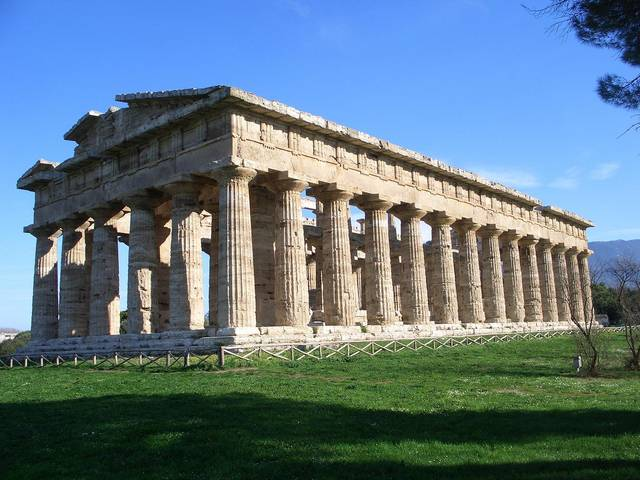
\includegraphics[scale=0.7]{imgs/tempioposeidone.jpg} 
\caption{Tempio di Poseidone\label{tempioposeidone}}
\end{center}
\end{figure}
Il secondo tempio è il \emph{Tempio di Poseidone} (fig. \ref{tempioposeidone}) e incarna il più riuscito esempio di architettura greca in Occidente. Costruito intorno al 450 a.C. seguendo lo stile architettonico dorico classico (lo stesso del Partenone di Atene) risulta orientato da ovest ad est. Il terzo ed ultimo grande tempio è il \emph{Tempio di Cerere}, costruito verso la fine del VI sec. a.C. nel punto più alto della città. Altri punti d'interesse minore sono il \emph{Templio Italico} (dedicato a Giove, Giunone e Minerva, era posto su un alto basamento al cui centro si ergeva un imponente altare e vi si poteva accedere solo dal lato a Sud tramite un'ampia gradinata), il \emph{Foro} (edificato dai romani sulla vecchia Agorà Greca), il \emph{Boleuterion} (detto anche Teatro Greco, fu costruito originariamente per ospitare le riunioni del massimo Consiglio della città ed aveva forma circolare prima di essere ridotto nelle dimensioni dai romani prima sul lato occidentale e poi sul lato settentrionale), l'\emph{Anfiteatro}(destinato agli spettacoli dei Gladiatori e risalente al primo secolo D.C.), il \emph{Ginnasio} (dotato di piscina per gare di nuoto) e il \emph{Sacello Ipogeico} (costruzione sotterranea rinvenuta nel 1954 di cui è ignota la finalità, si suppone che si tratti un tempio sotterraneo dedicato alla dea della fecondità e fertilità, oppure un cenotafio -una tomba simbolica- realizzata per onorare il fondatore della città).
\section{Obiettivi}
Lo scopo di questa tesi è quello di sviluppare, nel contesto di DATABENC, un'applicazione mobile che assista i turisti nella visita del sito archeologico degli scavi di Paestum.
Il turista potrà, sul suo dispositivo mobile, avere a disposizione una mappa su cui poter visualizzare la propria posizione e quella dei punti di interesse presenti nel sito.
Il turista potrà, inoltre, ottenere informazioni approfondite e materiale multimediale su tali punti di interesse e, all'occorrenza, consutarlo offline.
Sono previsti, inoltre diversi itinerari e percorsi guidati all'interno del sito.






\clearpage{\pagestyle{empty}\cleardoublepage}


%%%%%%%%%%%%%%%%%%%%%%%%%%%%%%%%%%%%%%%%%%%%%%%%%%%%%%%%%%%

\chapter{Architettura e tecnologie}
\label{ref:architettura}

Verranno introdotte le architetture e ele tecnologie di utilizzo

\section{Architettura Client/Server}
L'\emph{architettura client/server} indica un'architettura software che è costituita da due moduli integrati ma distinti, residenti generalmente su calcolatori diversi.\\
In una rete informatica ci si riferisce ai computer ad essa collegati come host o terminali, perché ospitano programmi di livello applicativo. 
Gli host, o nodi, sono ulteriormente suddivisi in due categorie, client e server. La condivisione delle risorse, che generalmente avviene attraverso la rete, tra i client e i server definisce l'architettura client/server (fig. \ref{clientserver}).

\begin{figure}[h]
\begin{center}
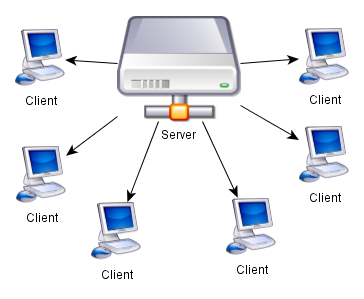
\includegraphics[scale=0.75]{imgs/clientserver.png} 
\caption{Architettura Client/Server\label{clientserver}}
\end{center}
\end{figure}

Il server svolge le operazioni necessarie per realizzare un servizio, mentre il client può effettuare alcune operazioni e quindi richiede un terminale con capacità elaborative. Tipicamente il client gestisce la porzione d'interfaccia utente dell'applicazione, verifica i dati inseriti e provvede ad inviare al server le richieste formulate dall'utente. Inoltre gestisce le risorse locali, come la tastiera, il monitor, la CPU, e le periferiche.
L'affermazione di questo modello è legata alla disponibilità di reti locali a basso costo ed alla diffusione della rete Internet, in cui i servizi seguono tale struttura.
In un ambiente client/server, sul computer client è in esecuzione un software applicativo detto programma client, il quale richiede e riceve un servizio da un programma server che viene eseguito sul computer server. 
Il programma client e il programma server interagiscono tra loro attraverso comunicazioni, ovvero scambiandosi messaggi attraverso la rete informatica. Quando un client si connette ad un server, gli invia una richiesta; il server, essendo in ascolto, la intercetta e l'interpreta effettuando le elaborazioni necessarie al suo soddisfacimento e restituisce un risultato sotto forma di risposta al client il quale lo visualizza all'utente.
Le applicazioni operanti in rete hanno protocolli di livello di applicazione che definiscono il formato e l'ordine dei messaggi scambiati tra i processi, così come definiscono le azioni da intraprendere alla trasmissione o alla ricezione dei messaggi.
A livello di applicazione, un protocollo definisce come i processi delle applicazioni, che funzionano su differenti terminali, si scambiano i messaggi, in particolare il protocollo specifica:
\begin{itemize}
\item i tipi di messaggi scambiati, per esempio, messaggi di richiesta e messaggi di risposta;
\item la sintassi dei vari tipi di messaggio, per esempio i campi del messaggio e come questi ultimi
vengono caratterizzati;
\item la semantica dei campi, cioè il significato dell'informazione nei campi;
\item le regole per determinare quando e come un processo invia messaggi o risponde a messaggi.
\end{itemize}


Prima di parlare dell'evoluzione del client/server è necessario fare una breve introduzione sulle componenti fondamentali di un'architettura di questo tipo.



Si distinguono tre parti principali di tale architettura: i dati sono la parte legata alla gestione delle informazioni persistenti, cioè quelle informazioni che si vuole mantenere nel tempo; la logica applicativa è rappresentata dai programmi veri e propri, ovvero quella parte del software che viene utilizzato per effettuare le operazioni per cui sono stati scritti; la presentazione, è quella parte del software che permette la comunicazione con l'utente.
\begin{figure}[h]
\begin{center}
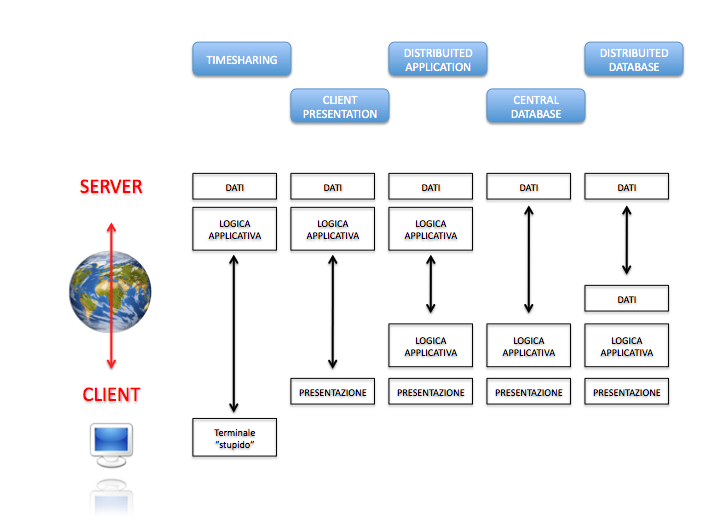
\includegraphics[scale=0.55]{imgs/clientserverorganization.png} 
\caption{Organizzazioni Client/Server\label{clientserverorganization}}
\end{center}
\end{figure}
L'architettura client/server ha avuto una evoluzione nel tempo (fig. \ref{clientserverorganization}) che l'ha portata attraverso vari stadi analizzati di seguito:
\begin{itemize}
\item \emph{Timesharing}: con questa soluzione, sul server sono presenti tutte e tre le parti fondamentali dell'architettura: dati, logica e presentazione. Il client è rappresentato da un terminale cosiddetto “stupido” il quale permette l'interazione con il server, senza avere una sua capacità elaborativa;
\item \emph{Client presentation}: dai tre livelli iniziali, viene staccata la presentazione che viene portata sul client, mentre la parte logica e quella dati, continuano a rimanere sul server;
\item \emph{Application distribution}: aumentando la potenza elaborativa dei client, si è pensato di spostare oltre che alla presentazione anche una parte della logica su quest'ultimo; questo tipo di operazione ha, da un lato, reso meno gravose le elaborazioni sui server, ma dall'altro ha aumentato i costi a causa dell'introduzione di nuovo software, in quanto necessita l'aggiornamento su ogni client su cui è installato. La caratteristica principale di questo stadio è che la parte di logica è distribuita in parte sul client e in parte sul server;
\item \emph{Central database}: il passo successivo è stato quello di spostare tutta la logica sul client insieme alla presentazione, lasciando sul server solo la parte dati. Questo tipo di soluzione ha il vantaggio di avere una banca dati centralizzata, ma lo svantaggio, per aziende molto grandi, è quello di avere un grande numero di accessi localizzati in un singolo punto;
\item \emph{Distribuited database}: per ovviare agli svantaggi della soluzione precedente si è pensato di portare sui client anche la parte dati. In questo modo si pone una soluzione al sovraccarico generato dal gran numero di utenti che si connettono ai dati, ma si crea un
altro problema legato alla sincronizzazione delle banche dati.
\end{itemize}



\subsection{Piattaforma Client}

I sistemi operativi per dispositivi mobili sono componenti software che garantiscono il funzionamento di dispositivi quali telefoni cellulari, smartphone, tablet, palmari e lettori MP3, coordinando e gestendo le risorse (hardware e software), e creando un'interfaccia con l'utente.
Diversamente dai sistemi operativi per desktop e laptop, essi devono affrontare problematiche critiche tra cui: limitatezza delle risorse (sia in termini di CPU che di memoria RAM), dimensioni ridotte dello schermo, sistemi touch-screen più o meno avanzati, tecnologie differenti per l'accesso ad Internet, consumo della batteria.
Nell'accezione moderna, il sistema operativo mobile non è solo un prodotto software, ma una vera e propria piattaforma, che mette a disposizione degli sviluppatori delle API su cui sviluppare applicazioni.

Un \emph{ecosistema mobile} è costituito dal sistema operativo, inteso come piattaforma, dagli sviluppatori, che incrementano il numero e migliorano la qualità delle applicazioni disponibili, e dagli utilizzatori, che acquistano sia la piattaforma che le applicazioni nello store.
In questo sezione verranno trattati i principali sistemi operativi mobile e i relativi framework per lo sviluppo delle applicazioni.


\subsubsection{Android}
Android (\emph{\url{http://www.android.com/}}), nato nel 2003, è il più diffuso sistema operativo per dispositivi mobili; open source; distribuito sotto licenza Apache, ovvero vi è la possibilità di modificare e distribuire liberamente il codice sorgente.\\
\begin{figure}
\begin{center}
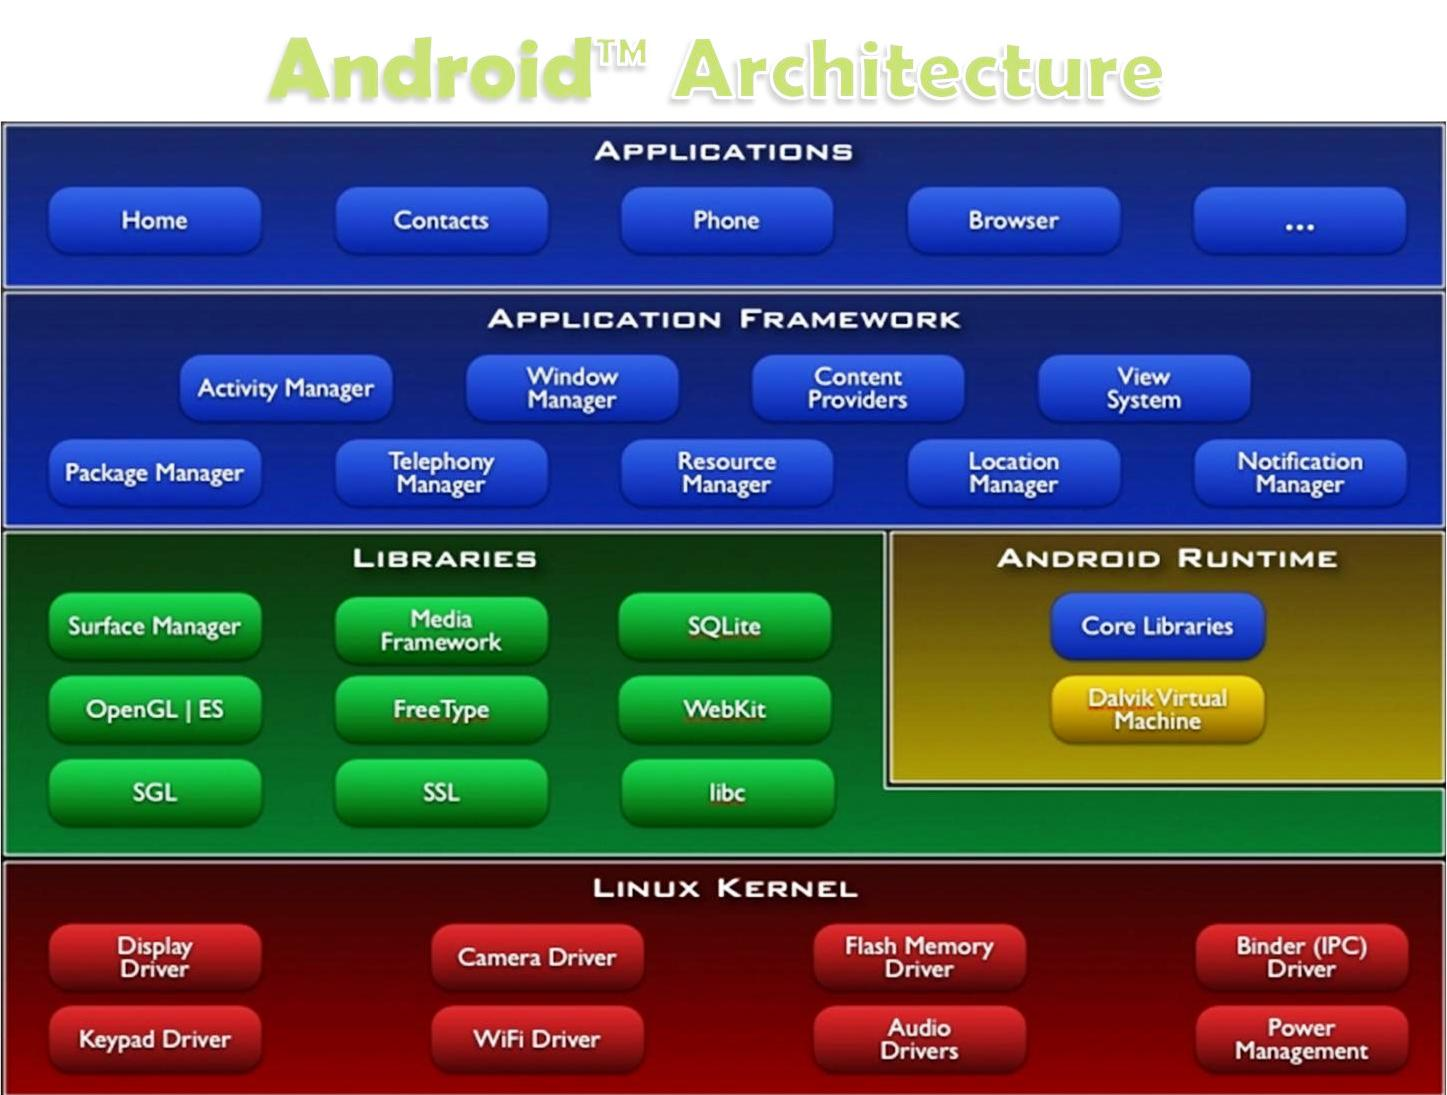
\includegraphics[scale=0.5]{imgs/android_architecture.jpg} 
\caption{Architettura del sistema operativo Android\label{androidarchitecture}}
\end{center}
\end{figure}

L'architettura Android, riportata in figura \ref{androidarchitecture}, è così definita:
\begin{itemize}
\item \emph{kernel}, basato sul kernel Linux(versioni 2.6 e 3.x), contiene i driver per il funzionamento del dispositivo;
\item \emph{strato middleware contenente Librerie ed API}: scritte in C o C++, sono le librerie che forniscono le funzionalità standard al dispositivo, ovvero gestione delle funzioni del display (Surface Manager), gestione dei media (Media Framework), fonts di sistema, DBMS (SQLite), web browser engine (WebKit), e numerose altre;
\item \emph{Android Runtime}: Contiene la Dalvik virtual machine, una macchina virtuale ottimizzata per sfruttare la poca memoria presente nei dispositivi mobili, e che consente di far girare diverse istanze della macchina virtuale contemporaneamente, nascondendo al sistema operativo sottostante la gestione della memoria e dei thread. E' presente, inoltre, un compilatore just-in-time che esegue il Dalvik dex-code, simile al bytecode Java;
\item \emph{Framework di applicazioni che include librerie java basate su Apache Harmony\footnote{Sito internet di riferimento http://harmony.apache.org/}},  costituito da una serie di componenti e API che eseguono numerosi compiti, tra i quali la gestione dell'interazione con l'utente (tramite l'Activity Manager), la condivisione delle informazioni tra i vari processi (Content Provider), gestione delle finestre (Window Manager), gestione delle funzionalità telefoniche (Telephony Manager), ottimizzazione delle risorse (Resource Manager), gestione del ciclo di vita delle applicazioni (Package Manager), gestione della localizzazione (Location Manager), gestione delle notifiche con l'utente (Notification Manager).
\end{itemize}

Per quanto riguarda gli aggiornamenti, Android ha un rapido ciclo di rilascio (nuove versioni ogni sei-nove mesi).
Gli aggiornamenti sono in genere di natura incrementale e apportano miglioramenti del software a intervalli regolari. Tra una major release e l'altra vengono messi a disposizione rilasci intermedi per risolvere problemi di sicurezza e altri bug del software.
\\


\paragraph{Sviluppo Applicazioni}
Tutte le applicazioni Android, dovendo basarsi sul framework di librerie Java, sono scritte in Java.

L'Android software development kit SDK (\emph{\url{http://developer.android.com/sdk/}}) include un insieme di tool di sviluppo, quali un debugger, librerie, un emulatore basato su QEMU (\emph{\url{http://wiki.qemu.org/}}), codici di esempio e tutorials.
Le piattaforme di sviluppo supportate includono computer con sistema operativo Linux, MAC OS X (dalla 10.5.8) e Windows (da XP).
L'IDE (Integrated Development Enviroment) ufficialmente supportato è ADT (Android Development Tools), basato su Eclipse (\emph{\url{http://www.eclipse.org/}}) ma, in ogni caso, è possibile sviluppare applicazioni Android anche con altri IDE.

\subsubsection{iOS}
iOS (\emph{\url{http://www.apple.com/it/ios/}}) è un sistema operativo di Apple, derivato da Unix BSD ed ha un microkernel XNU Mach basato su Darwin OS.
Nato nel 2007, è rilasciato sotto licenza APSL (Apple Public Source License), che consente agli utenti di migliorare il software ma non di rilasciarlo.\\

\begin{figure}[h!]
\begin{center}
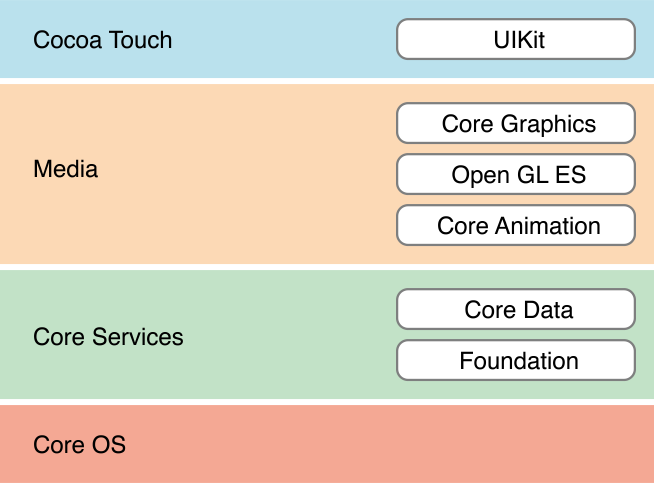
\includegraphics[scale=0.5]{imgs/ios_architecture.png} 
\caption{Architettura del sistema operativo iOS\label{iosarchitecture}}
\end{center}
\end{figure}

iOS ha quattro livelli di astrazione, riportati in figura \ref{iosarchitecture}:
\begin{itemize}
\item \emph{Core OS Layer}: contiene le caratteristiche di basso livello su cui sono basate la maggior parte delle tecnologie. Contiene il kernel ed interfacce di basso livello UNIX. Gestisce la memoria virtuale, i threads, il filesystem e i driver delle periferiche.
Sono presenti, inoltre, framework per l'esecuzione di DSP, calcoli di algebra lineare ed elaborazione delle immagini ; framework per la gestione del Bluetooth; framework per la gestione degli accessori hardware eventualmente connessi al dispositivo; framework per la sicurezza;
\item \emph{Core Services Layer}: contiene i servizi di sistema fondamentali che tutte le applicazioni usano. Offre quindi servizi di alto livello basati sui Core Service Frameworks, ad esempio lo storage di dati in remoto (iCloud); la protezione dei dati sensibili, per evitare che applicazioni malevole facciano uso di essi; la gestione dei documenti XML; la possibilità di condividere dati tra le varie applicazioni;
\item \emph{Media Layer}: contiene le tecnologie grafiche, audio e video;
\item \emph{Cocoa Touch Layer}: contiene i framework indispensabili per costruire applicazioni iOS (Cocoa Service Framework) e definisce l'infrastruttura di base ed il supporto per tecnologie fondamentali come il multitasking, l'input basato sul touch, le notifiche in push e locali e molti altri servizi di alto livello.
\end{itemize}

Apple rilascia aggiornamenti di iOS circa una volta l'anno. Tali aggiornamenti costituiscono revisioni complete del sistema operativo.
\paragraph{Sviluppo Applicazioni}
Le applicazioni per iOS possono essere sviluppate tramite l'iOS SDK (\emph{\url{http://developer.apple.com/}}),  disponibile solo su sistema operativo MAC OS X. Esse sono scritte in Objective-C, anche se esiste il supporto per C e C++.

L'IDE di riferimento per lo sviluppo di applicazioni per iOS è XCode, che include un editor di sorgenti; uno strumento per disegnare le interfacce utente; il compilatore LLVM  e un emulatore, oltre ad altri numerosi tool per il debug, il testing e la gestione degli errori.


\subsubsection{Windows Phone OS}
Windows Phone OS (\emph{\url{http://www.windowsphone.com/it-it}}) è un sistema operativo Microsoft, nato nel 2010, orientato ai dispositivi mobile. E' il successore di Windows Mobile, sistema operativo nato nel 1996 per i palmari, ma è completamente differente da quest'ultimo.

E' distribuito con licenza Microsoft EULA, per cui è soggetto a limitazioni d'uso, di garanzia e di responsabilità.

\begin{figure}
\begin{center}
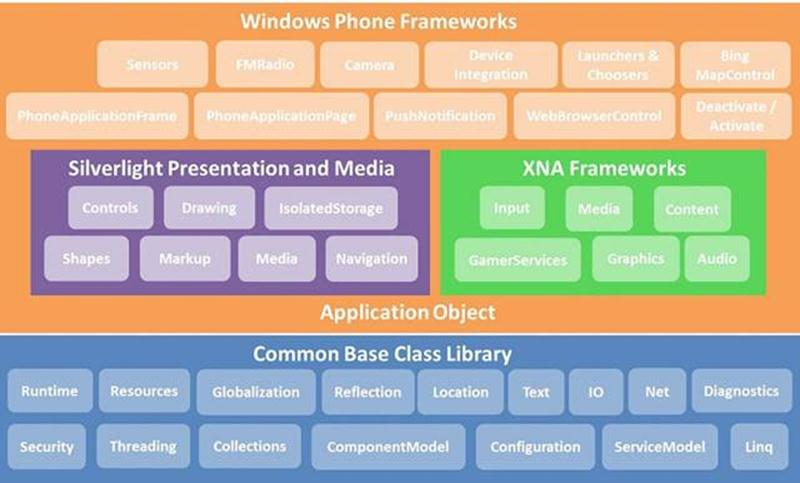
\includegraphics[scale=0.7]{imgs/windowsphone_architecture.jpg} 
\caption{Architettura del sistema operativo iOS\label{wparchitecture}}
\end{center}
\end{figure}

Windows Phone OS ha un'architettura a quattro livelli, come rappresentato in figura \ref{wparchitecture}:
\begin{itemize}
\item \emph{Common Base Class Library}: è una libreria standard che include un vasto numero di funzionalità comuni, come ad esempio la lettura e scrittura su un file, il rendering grafico, l'interazione con i database, la manipolazione di documenti XML e il supporto per il multithreading;
\item \emph{Silverlight Presentation and Media}: fornisce librerie per la navigazione, la grafica, la gestione dei media;
\item \emph{XNA Frameworks}: è un insieme di librerie, servizi e risorse per la gestione dell'accelerazione grafica e del rendering, dell'audio e dei servizi di autenticazione e connettività;
\item \emph{Windows Phone Frameworks}: definisce dei blocchi comuni per tutte le applicazioni Windows Phone. Esso fornisce l'interfaccia al sistema ed alle risorse hardware, ovvero i sensori, l'accelerometro, il compasso, il giroscopio e la fotocamera. In Windows Phone Framework è presente anche un sistema di notifiche.
\end{itemize}

\paragraph{Sviluppo Applicazioni}
Le applicazioni per Windows Phone possono essere scritte in C++, C\#, C, Visual Basic e HTML5, grazie al vasto supporto del framework .NET.
La più recente versione della Windows Phone SDK (\emph{\url{http://dev.windowsphone.com/}}) è disponibile solo per sistemi operativi Windows 8 a 64bit.

L'IDE di riferimento per lo sviluppo di applicazioni Windows Phone è Visual Studio per Windows Phone, che include un editor di sorgenti, di testing, di debug, di gestione delle risorse e del ciclo di vita dell'applicazione.
Microsoft mette inoltre a disposizione altri significativi tools come Express Blend, che permette di creare interfacce utente; Silverlight (\emph{\url{http://www.microsoft.com/silverlight/}}) e XNA per la gestione della grafica 2D e 3D; Windows Phone Emulator, l'emulatore dei dispositivi Windows Phone.\\

\subsubsection{Scelte}
Nella scelta dell'ecosistema su cui sviluppare e presentare un'applicazione per la visita dei siti culturali, \textbf{Windows Phone OS} è stato preferito agli altri, poiché si è tenuto conto di vari fattori:
\begin{itemize}
\item \textbf{originalità}: nello store di Windows Phone, non si trovano applicazioni simili, per cui essa costituirebbe il primo tentativo di visita assistita dei siti culturali;
\item \textbf{utilizzo dispositivi GPS}: l'utilizzo dei dispositivi GPS è molto semplice grazie alle API messe a disposizione da Microsoft;
 \item \textbf{background personale}.
\end{itemize}

\clearpage{\pagestyle{empty}\cleardoublepage}

\subsection{Codifica e serializzazione dei dati}
La serializzazione è un processo  per salvare un oggetto in un supporto di memorizzazione lineare o per trasmetterlo su una connessione di rete.
Essa può essere realizzata in modalità binaria o testuale.
La modalità binaria, seppur molto efficiente, presenta scarsa interoperabilità e flessibilità.
La serializzazione testuale, invece, essendo basata sulla tecnologia REST, determina un'ottimizzazione nello scambio di informazioni tra ambienti eterogenei, rendendo le strutture tradotte indipendenti dall'architettura e dalle differenti rappresentazioni dei dati.
I formati di serializzazione testuale più noti sono XML, JSON e YAML, che  sono trattati di seguito.

\subsubsection{XML}
La storia di XML (eXtra Markup Language)\footnote{Il formato XML è uno standard gestito dalla W3C. Il sito internet di riferimento è \emph{\url{http://www.w3.org/XML/}}} è strettamente legata a quella di SGML (Standard Generalized Markup Language), progetto ideato da IBM per migliorare l'interoperabilità aziendale, dal momento che la comunicazione tra computer era ostacolata da una ricca gamma di formati di file.

XML, infatti, è nato grazie ad una semplificazione di SGML per consentire di definire in maniera semplice nuovi linguaggi di markup da utilizzare in ambito web.
In definitiva, XML è un linguaggio marcatore basato su un meccanismo sintattico che consente di definire e controllare il significato degli elementi contenuti in un documento o in un testo.

\begin{figure}
\begin{center}
\lstset{language=MYXML}
\begin{lstlisting}
<?xml version="1.0" encoding="utf-8"?>
<!DOCTYPE Rubrica SYSTEM “Rubrica.dtd”>
<rubrica>
	<persona>
		<nome>Enrico</nome>
		<cognome>Bencivenga</cognome>
		<indirizzo>
			<via>Camillo Cucca 106</via>
			<cap>80031</cap>
			<citta>Brusciano</citta>
			<provincia>Napoli</provincia>
		</indirizzo>
	</persona>
</rubrica>

\end{lstlisting}
\caption{Esempio di documento XML\label{xmlimage}}
\end{center}
\end{figure}


\paragraph{Sintassi}
XML è una tecnologia adoperata per creare linguaggi di markup che descrivono dati di qualsiasi tipo, quindi consente di descrivere dati in modo accurato creando nuovi tag.
Un esempio di sintassi XML è l'esempio \textbf{Rubrica.xml} della figura \ref{xmlimage}.


Un documento XML si può quindi dividere in due sezioni: il \textit{prologo} e l'\textit{istanza}. 
Il prologo contiene informazioni di carattere generale sul documento, mentre l'istanza contiene i dati. Il documento XML è costituito da un insieme di dati e di marcatori che ne specificano la struttura.
Alcuni di essi sono:
\begin{itemize}
\item Tag;
\item Processing instructions;
\item Entità;
\item Commenti;
\item Sezione CDATA.
\end{itemize}

\subparagraph{Dichiarazione}
Le prime due righe contenute nell'esempio della figura \ref{xmlimage} costituiscono la dichiarazione del documento XML.
La prima riga contiene la specifica della versione di XML utilizzata e del tipo di codifica del documento. 
Nella seconda riga è stabilita la tipologia di documento alla quale appartiene il file, specificando il particolare schema DTD scelto.
La dichiarazione della tipologia di documento può essere di tre tipi:
\begin{itemize}
\item \textbf{Esterna}:
\lstset{language=MYXML}
\begin{lstlisting}
<!DOCTYPE ELEMENTO_ROOT SYSTEM "nomefile.dtd”>
\end{lstlisting}
\item \textbf{Interna}:
\begin{lstlisting}
<!DOCTYPE ELEMENTO_ROOT [CONTENUTO DTD SCHEMA]>
\end{lstlisting}
\item \textbf{Mista}:
\begin{lstlisting}
<!DOCTYPE ELEMENTO_ROOT SYSTEM "nomefile.dtd”
[CONTENUTO DTD SCHEMA]>
\end{lstlisting}
\end{itemize}

\subparagraph{Tag}
L'elemento radice della figura \ref{xmlimage} è il tag \textbf{<rubrica>}, che contiene all'interno tutti gli altri elementi del documento.
Inserire più di un elemento radice è considerato errato. I tag interni sono definiti elementi \textit{child}, e sono parte dell'organizzazione gerarchica di XML.
I tag di apertura e di chiusura vanno sempre specificati, tranne nel caso non vi siano informazioni in essi. Per gli elementi vuoti XML prevede una sintassi abbreviata \textbf{<tag/>}.

\subparagraph{Attributi}
I tag XML possono contenere informazioni interne che vengono definite \textit{attributi} del tag. Essi specificano proprietà intrinseche al tag e vanno indicati attraverso l'accoppiata nome-valore, come ad esempio:
\lstset{language=MYXML}
\begin{lstlisting}
<Telefono tipo="cellulare">3289196064</Telefono>
\end{lstlisting}.


\subparagraph{Commenti}
Oltre alle direttive di elaborazione, in un file XML è possibile individuare i commenti, racchiusi tra le sequenze di caratteri \textbf{<!--} e \textbf{-->}. Questi possono trovarsi in qualsiasi punto del documento, ed il testo contenuto non viene elaborato dal parser.


\begin{figure}[h]
\lstset{language=MYXML}
\begin{lstlisting}
<! ELEMENT persona (nome, cognome)>
<! ELEMENT nome (#PCDATA) >
<! ELEMENT cognome (#PCDATA) >
\end{lstlisting}
\caption{Esempio di file DTD\label{dtdimage}}
\end{figure}

\subparagraph{Correttezza sintattica e validità}
Un documento XML è valido se è conforme al DTD associato.
Un DTD (Document Type Definition) è uno strumento che definisce le componenti ammesse nella costruzione di un XML. Un esempio di DTD è riportato in figura \ref{dtdimage}.





Un documento XML, in ogni caso, non deve essere necessariamente valido, ma il requisito essenziale è la correttezza nella sintassi.
Tali regole sintattiche possono essere riassunte in:
\begin{itemize}
\item Deve essere presente un solo elemento radice;
\item I tag non possono iniziare con numeri o caratteri speciali e contenere spazi;
\item I tag devono essere innestati correttamente;
\item Tutti i tag e gli attributi sono espressi in minuscolo;
\item E' obbligatorio inserire i tag di chiusura, sia in forma estesa che in forma abbreviata, ove consentito.
\end{itemize}
Se un documento è sintatticamente valido, può essere analizzato da un \textit{parser}, un programma che, analizzando la struttura grammaticale del documento XML, ne ricostruisce l'albero a partire dall'elemento radice e proseguendo con gli elementi child.


\subsubsection{JSON}
JSON (JavaScript Object Notation) è un formato di serializzazione nato appositamente per lo scambio dei dati.
Un documento JSON è di facile interpretazione anche senza il processo di parsing, data la leggibilità della sua struttura.

JSON è completamente indipendente dal linguaggio di programmazione utilizzato, in quanto utilizza convenzioni conosciute dai programmatori di linguaggi della famiglia del C. 
Grazie a queste caratteristiche, JSON è un linguaggio ideale per lo scambio dei dati e per l'interoperabilità.
Con JSON è possibile rappresentare quattro tipi primitivi:
\begin{itemize}
\item numeri;
\item stringhe;
\item variabili booleane;
\item NULL.
\end{itemize}
e due tipi strutturati:
\begin{itemize}
\item array;
\item oggetti.
\end{itemize}

Il formato JSON è ampiamente diffuso, soprattutto tra gli sviluppatori web, per le dimensioni inferiori dello stream dati, dovute alla sua bassa ridondanza.

\paragraph{Sintassi}
La sintassi JSON è molto semplice e si basa su due strutture:
\begin{itemize}
\item \textbf{coppia nome/valore}, realizzabile in diversi linguaggi di programmazione come un oggetto, un record, uno struct, una tabella hash, un elenco di chiavi o un array associativo;
\item \textbf{elenco ordinato di valori}, realizzabile nella maggior parte dei linguaggi di programmazione con un array, un vettore, un elenco o una sequenza.
\end{itemize}
Queste due strutture sono utilizzabili in tutti i linguaggi di programmazione, e ciò rende ancora più evidente la natura di JSON, orientata all'interoperabilità.

\begin{figure}
\lstset{language=JSON}
\begin{lstlisting}
{"nome": "enrico"}
\end{lstlisting}
\caption{Esempio di oggetto JSON\label{jsonobjectimage}}
\end{figure}
\subparagraph{Oggetto}
Un oggetto in JSON è contenuto tra due parentesi graffe. Tra il nome e il valore sono presenti due punti ed il nome dell'oggetto è scritto tra due doppi apici, mentre il valore è scritto tra due doppi apici nel caso non sia numerico. Un esempio è in figura\ref{jsonobjectimage}.

\begin{figure}
\lstset{language=JSON}
\begin{lstlisting}
{"serializzazione": ["XML", "JSON", "altro"]}
\end{lstlisting}
\caption{Esempio di oggetto JSON\label{jsonarrayimage}}
\end{figure}

\subparagraph{Array}
Un array è una raccolta ordinata di valori. In JSON un array è contenuto tra due parentesi quadre e i valori sono separati da virgola, come è evidente dalla figura \ref{jsonarrayimage}.

Le stringhe sono rappresentate come nella maggior parte dei linguaggi di programmazione e vanno sempre messe tra doppi apici, mentre i numeri possono iniziare con identificatori di segno ed essere seguiti da una parte esponenziale, così come in molti linguaggi.
Solo le rappresentazioni esadecimali o ottali non sono permesse.
\begin{figure}
\lstset{language=JSON}
\begin{lstlisting}
{
  "rubrica": {
    "persona": {
      "nome": "Enrico",
      "cognome": "Bencivenga",
      "indirizzo": {
        "via": "Camillo Cucca 106",
        "cap": "80031",
        "citta": "Brusciano",
        "provincia": "Napoli"
      }
    }
  }
}
\end{lstlisting}
\caption{Esempio di oggetto JSON\label{jsonimage}}
\end{figure}

Nell'immagine \ref{jsonimage} è possibile visualizzare un esempio completo di file JSON, analogo a quello precedente di file XML in figura \ref{xmlimage}.
L'indentazione è utilizzata solo a scopo di chiarezza sintattica, ma il testo si estende su di una sola riga, senza caratteri di ritorno a capo.
Naturalmente anche un documento JSON può essere elaborato da un parser e ricostruito.

\subsubsection{YAML}
YAML (YAML Ain't Markup Language), sito web di riferimento \emph{\url{http://yaml.org}}, è un linguaggio nato nel 2001 con l'obiettivo di essere \textit{human-friendly}.
E' progettato per persone che lavorano con dati, grazie alla sua comprensibilità ed interoperabilità.
YAML è peraltro un linguaggio molto pulito, in quanto riduce al minimo la quantità di caratteri strutturali e permette di mostrare i dati in modo naturale e significativo.
Gli obiettivi di YAML sono:
\begin{itemize}
\item semplicità di lettura;
\item corrispondenza con i tipi per la maggioranza dei linguaggi di programmazione;
\item esportabilità dei dati;
\item estendibilità;
\item facilità di implementazione e usabilità.
\end{itemize}

\paragraph{Sintassi}
YAML mette a disposizione due tipi di sintassi, una indentata e una in linea, simile al formato JSON.
Inoltre in YAML ci sono degli indicatori che servono a descrivere la struttura ed il contenuto di un documento YAML.

\begin{figure}
\lstset{language=YAML}
\begin{lstlisting}
--- # Discipline
 - Matematica
 - Informatica
 - Fisica
\end{lstlisting}
\caption{Lista nel formato indentato YAML\label{yamllistaimage}}
\end{figure}

\begin{figure}
\lstset{language=YAML}
\begin{lstlisting}
 --- # Discipline
 [Matematica, Informatica, Fisica]
\end{lstlisting}
\caption{Lista nel formato convenzionale YAML\label{yamllistbimage}}
\end{figure}

\begin{figure}
\lstset{language=YAML}
\begin{lstlisting}
--- # Blocco indentato
   nome: Enrico Bencivenga
   eta: 30
 --- # Blocco allineato
 {nome: Enrico Bencivenga, eta: 30}
\end{lstlisting}
\caption{Array in YAML\label{yamlarrayimage}}
\end{figure}

\begin{figure}
\lstset{language=YAML}
\begin{lstlisting}
 --- |
	Questa è la 
		tesi di laurea
			in Ingegneria Informatica
		di Enrico Bencivenga
	matr. 534000442
\end{lstlisting}
\caption{Stringa nel formato indentato YAML\label{yamlstringaimage}}
\end{figure}

\begin{figure}
\lstset{language=YAML}
\begin{lstlisting}
 --- >
Questa è la 
tesi di laurea
in Ingegneria Informatica
di Enrico Bencivenga
matr. 534000442
\end{lstlisting}
\caption{Stringa nel formato convenzionale YAML\label{yamlstringbimage}}
\end{figure}

\subparagraph{Liste}
Le liste sono collezioni di elementi. La loro rappresentazione in YAML può essere indentata (fig. \ref{yamllistaimage}) o allineata (fig. \ref{yamllistbimage}).

\subparagraph{Array associativi}
Gli array sono associazioni nome/valore, e possono essere rappresentati come in figura \ref{yamlarrayimage}.

\subparagraph{Stringhe}
Le stringhe non richiedono gli apici o i doppi apici per essere rappresentate.

La rappresentazione delle stringhe può essere indentata, come nella figura \ref{yamlstringaimage}, oppure allineata, come nella figura \ref{yamlstringbimage}, dove il testo viene allineato in un singolo paragrafo.

\subsubsection{Scelte}
JSON è caratterizzato dalla semplicità di rappresentazione delle strutture dati e da una bassa ridondanza, dovuta all'assenza dei tag di chiusura; è molto facile da interpretare e per questo si adatta alle applicazioni web-based.\\

YAML ha caratteristiche aggiuntive rispetto a JSON, quali l'estensibilità dei tipi, la rappresentazione di stringhe senza apici, gli anchors e gli aliases. Anche YAML risulta molto adatto alle applicazioni web-based.\\
XML ha più vincoli di YAML e JSON, poichè è nato per essere compatibile con SGML, ma risulta più adatto alla descrizione di strutture dati e presenta uno spettro di utilizzo più vasto.

\clearpage{\pagestyle{empty}\cleardoublepage}

\subsection{Tecniche di geolocalizzazione}
La geolocalizzazione è l'identificazione della posizione geografica di un dato oggetto nel mondo reale.
Gli oggetti possono essere telefoni cellulari, pc, tablet, palmari e ci sono diverse tecniche, indoor ed outdoor.
\begin{itemize}
\item \textbf{outdoor}: localizzazione satellitare;
\item \textbf{indoor}: infrastrutture ad-hoc e WiFI;
\item \textbf{indoor ed outdoor}: infrastruttura cellulare.
\end{itemize}
Vi sono inolte diversi metodi per valutare la qualità di un sistema di localizzazione:
\begin{itemize}
\item \textbf{Errore medio}: corrispondenza tra la posizione stimata e quella reale;
\item \textbf{Probabilità di corretta locazione}: probabilità di localizzare l'obiettivo entro una determinata soglia;
\item \textbf{Rendimento}: capacità del metodo a stimare la posizione in tutti i tipi di ambienti;
\item \textbf{Consistenza}: misura della stabilità dell'errore medio in ambienti differenti;
\item \textbf{Overhead}: quantità di informazione scambiata tra il terminale ed il sistema;
\item \textbf{Consumo di potenza}: quantita delle risorse energetiche impiegate;
\item \textbf{Latenza}: intervallo di tempo tra la richiesta di posizionamento e la risposta del sistema;
\item \textbf{Costi roll-out}: costi necessari all'installazione dell'infrastruttura;
\item \textbf{Costi operativi}: costi legati al mantenimento dell'infrastruttura.
\end{itemize}

\subsubsection{Localizzazione satellitare}
La localizzazione satellitare si basa su infrastrutture indipendenti dedicate, ovvero un certo numero di satelliti utilizzati solo a questo scopo e di tipo terminal-based.
I vantaggi del posizionamento satellitare sono la copertura globale e l'alto livello di accuratezza, ma è soggetto anche ad importanti inconvenienti, come un eccessivo consumo dovuto ai dispositivi che utilizzano il segnale GPS e ai disturbi naturali che possono ostacolarne la ricezione.

\paragraph{GPS}
Il sistema GPS (Global Positioning System)\footnote{Il sito di riferimento per lo standard GPS è \emph{\url{http://www.gps.gov}}.}, avviato dagli USA negli anni '70 e completato nel 1993, è stato realizzato per motivi essenzialmente militari, al fine di consentire il percorso dei mezzi militari, sia sulla terraferma che in mare in modo da localizzarne la posizione in ogni momento e consentire eventuali operazioni di supporto e salvataggio.
Il GPS utilizza dai 24 ai 32 satelliti artificiali, divisi in gruppi da 4, che ruotano attorno alla terra a circa 20.200 km in orbite che formano tra loro angoli di 60 gradi.

\begin{figure}
\begin{center}

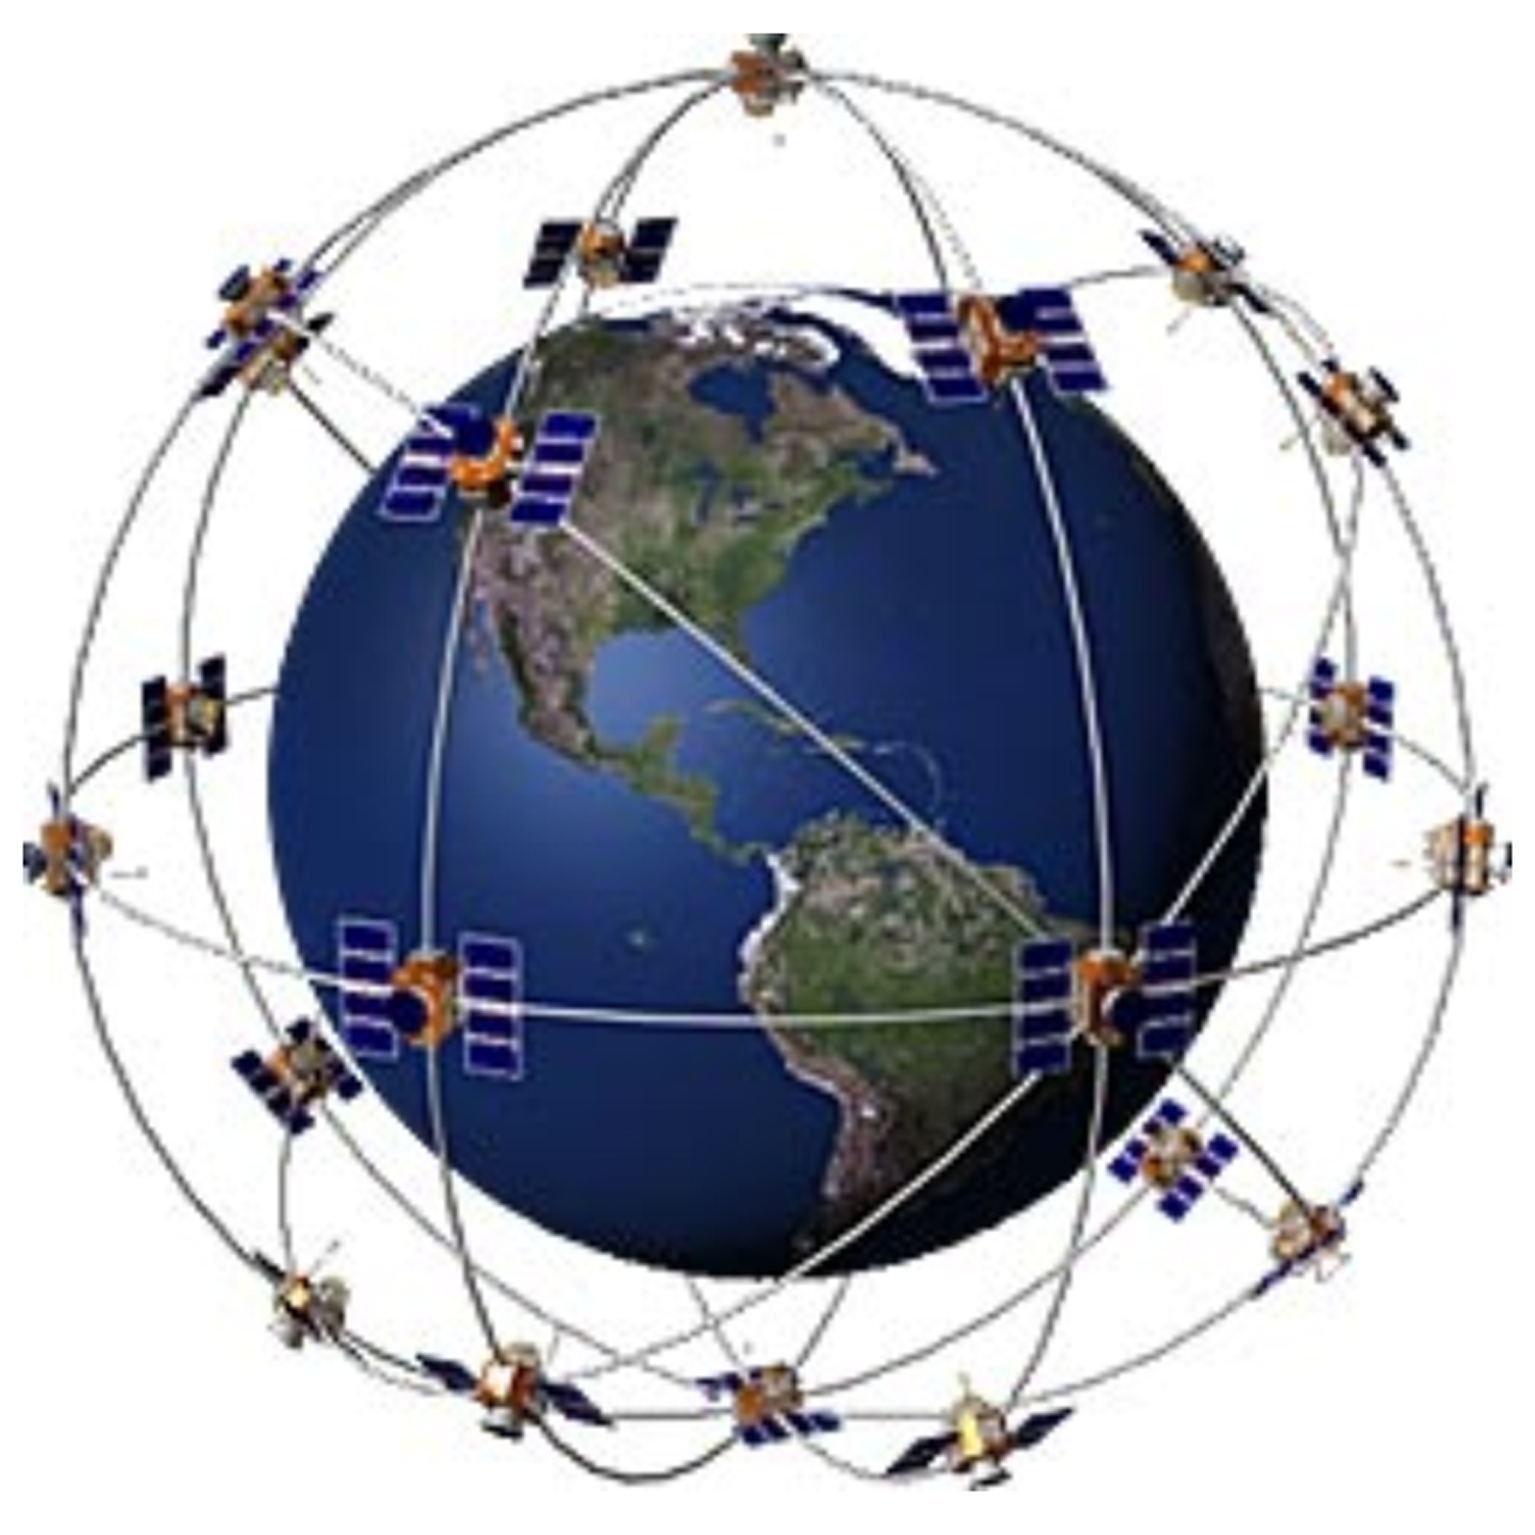
\includegraphics[scale=0.3]{imgs/gpssatelliteimage.jpg}
\caption{Rappresentazione dei satelliti GPS in orbita intorno alla terra\label{gpsimage}}
\end{center}

\end{figure}

\subparagraph{Principi di funzionamento}
Il sistema GPS è nato come versione satellitare e perfezionamento del sistema LORAN, nato negli USA attorno al 1940, che consentiva la determinazione della posizione lungo le rotte di grande traffico navale ed aereo, utilizzando un grande numero di stazioni terrestri.

Il sistema GPS, così come il LORAN, consente di determinare la propria posizione sulla superficie terrestre e la propria altitudine in qualunque punto ci si trovi tramite un ricevitore GPS, il quale intercetta a terra il segnale generato dai satelliti in orbita che passano sopra di noi, così come rappresentato in figura \ref{gpsimage}.
Infatti, visto il numero, l'orbita ed il periodo di rotazione, in ogni istante e in ogni punto terreste è possibile intercettare il segnale generato da 6 a 12 satelliti.

\subparagraph{Satelliti}
Le funzioni dei satelliti possono essere così sintetizzate:
\begin{itemize}
\item trasmettere informazioni agli utilizzatori mediante un segnale radio;
\item mantenere un riferimento di tempo accurato, grazie agli orologi di bordo;
\item ricevere e memorizzare informazioni dal segmento di controllo;
\item eseguire manovre e correzioni di orbita.
\end{itemize}

\subparagraph{Ricevitore}
I ricevitori GPS commerciali, dal costo molto contenuto, consentono di sintonizzarsi automaticamente sulle frequenze dei satelliti GPS e, dopo un tempo di ricerca relativamente breve, di determinare la propria posizione ed, eventualmente, la propria quota, elaborando le distanze di almeno quattro satelliti.
Nei navigatori GPS per auto e negli smartphone, il risultato dell'elaborazione viene mostrato come punto all'interno di una cartina geografica completa, che può essere ingrandita fino a diventare una vera e propria cartina topografica.

\subparagraph{Precisione}
La precisione della ricezione GPS è influenzata da una serie di fattori, tra cui la posizione dei satelliti, l'eventuale presenza di rumore del segnale radio, le condizioni atmosferiche e le barriere naturali.
In generale, tali disturbi possono introdurre errori di precisione tra 1 e 10 metri.
La determinazione  più accurata della  posizione si verifica quando il satellite e il ricevitore GPS sono in vista tra loro senza  nessun altro oggetto schermante. Sotto questa ipotesi, il margine di errore del posizionamento è di circa 90 cm.

\subsubsection{Localizzazione cellulare}
La localizzazione cellulare è utilizzata nelle reti cellulari, come GSM o UMTS, per ricavare la posizione di un utente.
Questo sistema di localizzazione è utilizzato per ricavare la presenza di un utente all'interno di una cella, per cui è soggetto a margini di errore abbastanza ampi.
Per questo motivo, i gestori hanno predisposto nuovi strumenti per equipaggiare le proprie reti con dispositivi e protocolli finalizzati alla realizzazione del posizionamento in modo più accurato ed efficiente.
A tal proposito, diversi metodi sono stati specificati dai gruppi di standardizzazione, come 3GPP (\emph{\url{http://www.3gpp.org}}. La maggior parte di questi metodi è network-based, per cui anche i dispositivi più datati possono usufruirne.
Il vantaggio di questi sistemi di localizzazione cellulare è che possono essere utilizzati anche in ambienti chiusi, diversamente dai sistemi satellitari.
Il posizionamento cellulare può essere molto costoso per quanto riguarda l'overhead dovuto alla segnalazione, soprattutto se è richiesto un alto grado  di accuratezza e, inoltre, la capacità impiegata per la localizzazione è indisponibile per i servizi voce e dati.

\subsubsection{Localizzazione indoor}
La localizzazione indoor è nata per essere utilizzata all'interno di grandi edifici, campus universitari, strutture museali, strutture ospedaliere e uffici di vario genere.
E' basata su tecnologie radio, infrarossi o ad ultrasuoni, con un raggio di comunicazione evidentemente limitato.
La realizzazione di un sistema di localizzazione indoor può avvenire mediante la realizzazione di infrastrutture dedicate o l'utilizzo di infrastrutture preesistenti, come le reti WLAN.
La localizzazione indoor ha il vantaggio di presentare un basso consumo di potenza dei dispositivi utilizzati per la ricezione e l'elevata accuratezza dovuta al corto raggio delle tecnologie usate.

Esistono diverse soluzioni commerciali per la localizzazione indoor, come \textbf{RADAR} (\emph{\url{http://research.microsoft.com/en-us/projects/radar/}}), sviluppata da Microsoft, che è un sistema a radio frequenza; \textbf{Real Time Location System - RTLS} (\emph{\url{http://www.ekahau.com/real-time-location-system/technology}}), di Ekahau, che si basa sull'infrastruttura WLAN IEEE 802.11; \textbf{Visibility System} (\emph{\url{http://www.aeroscout.com/technology}}), di Aeroscout, basato sempre sull'infrastruttura WLAN IEEE 802.11; \textbf{Wireless Location Appliance} (\emph{\url{http://www.cisco.com/en/US/products/ps6386/index.html}}), di Cisco, basato su WLAN.

\subsubsection{Scelte}
Nell'ambito di studio, la scelta operata è sulla tecnologia \textbf{GPS}, per i seguenti motivi:
\begin{itemize}
\item \textbf{impossibilità di utilizzo localizzazione indoor}: date le dimensioni considerevoli del sito archeologico, si è ritenuto improbabile l'installazione di una rete WiFi che coprisse tutta l'area, al fine di localizzare tutti i dispositivi presenti;
\item \textbf{inutilità localizzazione cellulare}: la localizzazione cellulare è soggetta a margini di errore ampi per cui, nell'ambito del caso in questione, in cui vi è la necessità di individuare con margini d'errore ridotti la posizione corretta, risulta inutile;
\item \textbf{elevata precisione}: i margini di errore del GPS sono piuttosto bassi, come trattato nel capitolo \ref{tecnologie}.
\end{itemize}


\clearpage{\pagestyle{empty}\cleardoublepage}

\subsection{Codifica e serializzazione dei dati georeferenziati}
\subsubsection{GeoRSS}
GeoRSS è uno standard emergente per la codifica delle informazioni come parte di un feed Web, infatti il nome \emph{GeoRSS} deriva proprio da \emph{RSS}, il più conosciuto feed Web.
Il GeoRSS, il contenuto riguardante la posizione consiste di punti geografici, linee e poligoni e delle relative descrizioni, come mostrato in fig. \ref{georssimage}. Tali feed sono progettati per essere utilizzati da software geografici come i generatori di mappe.

\begin{figure}
\begin{center}
\lstset{language=MYXML}
\begin{lstlisting}
 <?xml version="1.0"?>
 <?xml-stylesheet href="/eqcenter/catalogs/rssxsl.php?feed=eqs7day-M5.xml" type="text/xsl" 
                  media="screen"?>
 <rss version="2.0" 
      xmlns:geo="http://www.w3.org/2003/01/geo/wgs84_pos#" 
      xmlns:dc="http://purl.org/dc/elements/1.1/">
  <channel>
     <title>USGS M5+ Earthquakes</title>
     <description>Real-time, worldwide earthquake list for the past 7 days</description>
     <link>http://earthquake.usgs.gov/eqcenter/</link>
     <dc:publisher>U.S. Geological Survey</dc:publisher>
     <pubDate>Thu, 27 Dec 2007 23:56:15 PST</pubDate>
     <item>
       <pubDate>Fri, 28 Dec 2007 05:24:17 GMT</pubDate>
       <title>M 5.3, northern Sumatra, Indonesia</title>
       <description>December 28, 2007 05:24:17 GMT</description>
       <link>http://earthquake.usgs.gov/eqcenter/recenteqsww/Quakes/us2007llai.php</link>
       <geo:lat>5.5319</geo:lat>
       <geo:long>95.8972</geo:long>
     </item>
   </channel>
 </rss>
\end{lstlisting}
\caption{Esempio di documento GeoRSS\label{georssimage}}
\end{center}
\end{figure}
Le due codifiche principali di GeoRSS sono GeoRSS-Simple e GeoRSS Geography Markup Language. Il primo è un formato leggerissimo che supporta geometrie semplici (punti, linee, poligoni) e può essere utilizzato per gli scopi tipici di geolocalizzazione. GeoRSS GML è un formato dell'Open Geospatial Consortium (OGC) GML Application Profile, e supporta un vastissimo range di caratteristiche rispetto a GeoRSS Simple.
E' presente anche un formato di serializzazione GeoRSS definito dalla W3C, ma è obsoleto e parzialmente deprecato, pur essendo ancora il più utilizzato.

\clearpage{\pagestyle{empty}\cleardoublepage}

\subsection{Rappresentazione dei dati georeferenziati}
Il Web Mapping è un processo di progettazione, implementazione, generazione e produzione di mappe sul web.
Un caso particolare di mappe web sono le mappe mobili, visualizzate su periferiche mobili, come telefonini, smartphone, tablet e GPS.

I vantaggi derivanti dall'utilizzo di mappe web sono:
\begin{itemize}
\item facilità di generazione di mappe aggiornate;
\item economicità dell'infrastruttura software ed hardware;
\item facilità di distribuzione degli aggiornamenti;
\item supporto e compatibilità con la maggior parte dei browser e dei sistemi operativi;
\item facilità di personalizzazione;
\item supporto per l'hyperlinking di punti di interesse;
\item facilità di integrazione con altri oggetti multimediali.
\end{itemize}

I servizi di web mapping più noti sono \textbf{Google Maps} e \textbf{Bing Maps}.
\subsubsection{Google Maps}
Google Maps (\emph{\url{https://maps.google.it}}) è un servizio di web mapping nato nel 2005 e fornito da Google, che include numerosi altri servizi basati sulle mappe (mappe stradali, pianificazione di percorsi e localizzazione di imprese).
Le mappe non sono aggiornate in tempo reale, ma spesso dopo mesi o anni.
\paragraph{Google Maps API}
Google ha messo a disposizione le proprie API per consentire agli sviluppatori di integrare Google Maps all'interno dei loro siti web.
Il servizio offerto è gratuito, anche se Google si riserva, nei termini di licenza, di introdurre future forme di pagamento.

\subsubsection{Bing Maps}
Bing Maps (\emph{\url{http://it.bing.com/maps/}}) è un servizio di web mapping nato nel 2009 e distribuito da Microsoft nella \textit{Bing suite}.
Fornisce numerose tipologie di mappe: stradali, satellitari, aeree, tridimensionali, oltre che, naturalmente, servizi di traffico e di ricerca delle imprese.
\paragraph{Bing Maps API}
Microsoft, oltre a mettere a disposizione le Bing API agli sviluppatori, fornisce anche una SDK disponibile su più piattaforme, per realizzare applicazioni integrabili con la maggior parte dei prodotti commerciali Microsoft.
\subsubsection{Scelte}
La scelta di Windows Phone OS come piattaforma ha reso quasi obbligatoria l'adozione delle mappe di Bing Maps, che sono supportate nativamente dalla Windows Phone SDK.

\clearpage{\pagestyle{empty}\cleardoublepage}

\subsection{Web Service e protocolli di scambio delle informazioni}
Un \textit{Web Service} è, secondo la definizione data dal \textit{W3C}, un sistema software progettato per supportare l'interoperabilità tra diversi elaboratori su di una medesima rete ovvero in un contesto distribuito. L'interoperabilità è ottenuta associando all'applicazione un'interfaccia software (descritta in formato automaticamente elaborabile, ad esempio il Web Services Description Language), che espone all'esterno i servizi associati e utilizzando la quale altri sistemi possono interagire con l'applicazione stessa, attivando le operazioni descritte nell'interfaccia tramite appositi messaggi di richiesta.
Tali messaggi sono formattati secondo gli standard XML ed incapsulati e trasportati tramite i protocolli web (di solito HTTP), da cui il nome web service. Un esempio di trasporto è in figura \ref{webservice}.
\begin{figure}
\begin{center}
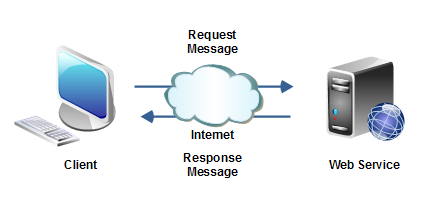
\includegraphics[scale=1]{imgs/webservice.png} 
\caption{Scambio messaggi in un Web Service\label{webservice}}
\end{center}
\end{figure}
I \textit{Web Service} hanno ridefinito nel tempo il modo in cui viene utilizzato il Web, che è visto non più come strumento di pubblicazione e consultazione di pagine statiche, ma anche e soprattutto come strumento per elaborare dati, interagire, integrare le applicazioni e creare business.
Questa nuova generazione di applicazioni internet consente ai privati di accedere a servizi studiati appositamente per le loro esigenze, ed alle aziende di comunicare e gestire i rapporti con clienti, partner e fornitori in modo semplice e immediato.
L'accesso ai Web Service è possibile da qualunque dispositivo in grado di interagire con la rete, ovvero PC, smartphone, palmari o notebook.\\
Un Web Service può essere scritto in qualsiasi linguaggio di programmazione e, come tutte le applicazioni web, ha la caratteristica fondamentale di trasmettere informazioni in formato testuale attraverso protocolli di tipo request-reply (HTTP).
Solitamente, un Web Service comunica con i browser tramite pagine HTML, incapsulate all'interno di una risposta HTTP; diversamente, nella comunicazione tra Web Service o tra Web Service e applicazioni le informazioni sono scambiate in maniera strutturata (cioè capaci di autodescriversi in modo da essere comprensibili sia ad un agente software che ad un umano).
I formati di descrizione sono naturalmente i formati di serializzazione dei dati trattati precedentemente, ovvero XML, JSON e YAML, la cui caratteristica principale è quella di essere testi semplici da cui estrarre informazioni tramite il parsing.\\
I protocolli per i web service utilizzano tre architetture diverse:
\begin{itemize}
\item \textbf{RPC oriented};
\item \textbf{Message oriented};
\item \textbf{REST}.
\end{itemize}
\subsubsection{RPC oriented}
L'architettura RPC oriented è basata sul concetto ri Remote Procedure Call dei middleware tradizionali.
Quindi, il client invia al server una richiesta, contenente il nome della procedura remota da invocare e i parametri, usando l'operazione POST del protocollo HTTP; Il server invia il risultato al client come risposta HTTP.
\paragraph{XML-RPC}
Il primo protocollo specificamente sviluppato per i Web Service è stato \textit{XML-RPC}, in cui la richiesta e la risposta del messaggio sono formulate in linguaggio XML.
XML-RPC sfrutta la disponibilità di parser XML su tutte le principali piattaforme e la facilità con cui si possono generare documenti XML.
Le principali carenze di XML-RPC sono l'assenza di meccanismi per la gestione di tipi di dato non supportati; il mancato supporto nativo di funzionalità avanzate come autenticazione e gestione delle transazioni; mancanza di definizione formale delle interfacce delle procedure remote, per cui eventuali errori o incongruenze sono scoperti solo a tempo di esecuzione.
Per ovviare a tali limiti è stato introdotto \textbf{SOAP}
\paragraph{SOAP}
Acronimo di \textit{Simple Object Access Protocol}, SOAP (\emph{\url{www.w3.org/TR/soap/}}) è basato su XML ed è accattato come standard dal consorzio W3C.
SOAP è supportato dai principali ambienti di sviluppo e ha la caratteristica di separare il formato dei messaggi dal modo in cui sono veicolati attraverso un protocollo già esistente. 
SOAP può utilizzare protocolli diversi da HTTP, come SMTP.
I vantaggi dell'utilizzo di SOAP, rispetto ad XML-RPC sono prevalentemente nella versatilità, dal momento che SOAP consente di estendere l'insieme dei tipi da usare come parametri e valori di ritorno e consente di estendere il protocollo stesso al fine di aggiungere funzionalità come la sicurezza o la gestione delle transizioni senza perdere l'interoperabilità.
Per la definizione formale dell'interfaccia, SOAP ricorre a \textbf{WSDL}.
\paragraph{WSDL}
WSDL, ovvero \textit{Web Service Description Language} è un linguaggio per definire le interfacce dei Web Service basati su SOAP.
Anch'esso è uno standard W3C ed è naturalmente basato su XML.
Un documento WSDL contiene una specifica "machine-readable" di:
\begin{itemize}
\item punti di accesso ai web service
\item protocolli utilizzati
\item operazioni disponibili, con i rispettivi parametri di ritorno
\item tipi non predefiniti usati dalle operazioni
\end{itemize}
Anche se in teoria un documento WSDL dovrebbe essere in un formato leggibile e modificabile da un essere umano, in pratica il formato è piuttosto complesso e si rende necessaria la generazione del documento tramite appositi tool e librerie, offerti dai principali ambienti di sviluppo.
Tipicamente il WSDL è disponibile online sul sito che ospita il web service ed è utilizzato a tempo di esecuzione sia per verificare che non ci siano modifiche dell'interfaccia server, sia per creare le classi che rappresentano la comunicazione col client.
Un esempio di WSDL è riportato in figura \ref{wsdlimage}.
\begin{figure}[h!]
\begin{center}
\lstset{language=MYXML}
\begin{lstlisting}
<?xml version="1.0"?> 
<wsdl:description xmlns:wsdl="http://www.w3.org/ns/wsdl"
  xmlns:wsoap= "http://www.w3.org/ns/wsdl/soap"
  xmlns:hy="http://www.herongyang.com/Service/"
  targetNamespace="http://www.herongyang.com/Service/">

  <wsdl:documentation>
    Hello_WSDL_20_SOAP.wsdl
    Copyright (c) 2009 by Dr. Herong Yang, herongyang.com
    All rights reserved
  </wsdl:documentation>

  <wsdl:types>
    <xsd:schema xmlns:xsd="http://www.w3.org/2001/XMLSchema"
      targetNamespace="http://www.herongyang.com/Service/">
      <xsd:element name="Hello" type="xsd:string"/>    
      <xsd:element name="HelloResponse" type="xsd:string"/>    
    </xsd:schema>    
  </wsdl:types>

  <wsdl:interface name="helloInterface" >
    <wsdl:operation name="Hello" 
      pattern="http://www.w3.org/ns/wsdl/in-out" 
      style="http://www.w3.org/ns/wsdl/style/iri">
      <wsdl:input messageLabel="In" 
        element="hy:Hello" />
      <wsdl:output messageLabel="Out" 
        element="hy:HelloResponse" />
    </wsdl:operation>
  </wsdl:interface>

  <wsdl:binding name="helloBinding" 
    interface="hy:helloInterface"
    type="http://www.w3.org/ns/wsdl/soap"
    wsoap:protocol="http://www.w3.org/2003/05/soap/bindings/HTTP/">
    <wsdl:operation ref="hy:Hello" 
      wsoap:mep="http://www.w3.org/2003/05/soap/mep/soap-response"/>
  </wsdl:binding>

  <wsdl:service name="helloService" 
    interface="hy:helloInterface">
    <wsdl:endpoint name="helloEndpoint" 
      binding="hy:helloBinding"
address="http://www.herongyang.com/Service/Hello_SOAP_12.php"/>
  </wsdl:service>

</wsdl:description>
\end{lstlisting}
\caption{Esempio di documento WSDL\label{wsdlimage}}
\end{center}
\end{figure}
La combinazione SOAP+WSDL consente di realizzare web service con uno sforzo di programmazione contenuto, sia lato client che lato server e, grazie all'uso del servizio \textbf{UDDI}, garantisce ed aumenta l'interoperabilità.
\paragraph{UDDI}
UDDI (\textit{Universal Description Discovery and Integration}) è un web service basato su SOAP+WSDL che realizza un repository di descrizioni WSDL con funzioni di pubblicazione e ricerca di web service in base ad una serie di metadati.
Lo standard UDDI originariamente ipotizzava lo sviluppo di un \textit{Universal Business Registry} pubblivo che consentisse una ricerca globale dei web service, ma attualmente l'idea dell'UBR è stata abbandonata ed il servizio UDDI è utilizzato soprattutto in abito intranet come repository centralizzato di documenti WSDL.
\subsubsection{Message oriented}
In un'architettura di servizi Message oriented le diverse applicazioni si scambiano messaggi unidirezionali che hanno le seguenti caratteristiche:
\begin{itemize}
\item il focus è sul messaggio più che sull'operazione;
\item se una richiesta genera una risposta, questa è inviata con un messaggio indipendente dal messaggio di richiesta;
\item il servizio non è tenuto a elaborare i messaggi che riceve in ordine di ricezione;
\item è sfumata la distinzione tra client e server: l'architettura è peer-to-peer.
\end{itemize}

I vantaggi dell'utilizzo di un'architettura Message oriented sono il disaccoppiamento anche temporale tra client e server, infatti, se il server non è momentaneamente disponibile, il messaggio può essere mantenuto in una coda; la maggiore flessibilità nella distribuzione (smistamento intelligente dei messaggi tra più server); flessibilità nell'ordine delle operazioni (priorità diverse per i messaggi).

\subsubsection{REST}
Representational state transfer (REST)\footnote{Il paradigma REST è stato introdotto nel 2000 nella tesi di dottorato di Roy Fielding, reperibile all'indirizzo \emph{\url{http://www.ics.uci.edu/~fielding/pubs/dissertation/rest_arch_style.htm}}} è un tipo di architettura software per i sistemi di ipertesto distribuiti come il World Wide Web.
Esso si riferisce ad un insieme di principi di architetture di rete, i quali delineano come le risorse sono definite e indirizzate. Il termine è spesso usato nel senso di descrivere ogni semplice interfaccia che trasmette dati su HTTP senza un livello opzionale come SOAP o la gestione della sessione tramite i cookie.

Le applicazioni basate sui principi REST, spesso definite "RESTful", usano richieste HTTP per inviare dati (creare o aggiornare), leggere dati (eseguire query) e cancellare dati.

Nel dettaglio, lo stile architetturale di REST, rappresentato in figura \ref{restimage}, consiste di un lato client e un lato server: i client inviano richieste ai server; i server elaborano tali richieste e restituiscono ai client i risultati delle elaborazioni.
Richieste e risposte si basano sul trasferimento di rappresentazioni di \textbf{risorse}.

L'esistenza delle risorse è un concetto importante in REST, in quanto esse sono fonti di informazioni a cui si può accedere tramite un identificatore globale (un URI). Per utilizzare le risorse, le componenti di una rete (client e server) comunicano attraverso una interfaccia standard (ad es. HTTP) e si scambiano rappresentazioni di queste risorse (il documento che trasmette le informazioni).
\\
\begin{figure}[h!]
\begin{center}
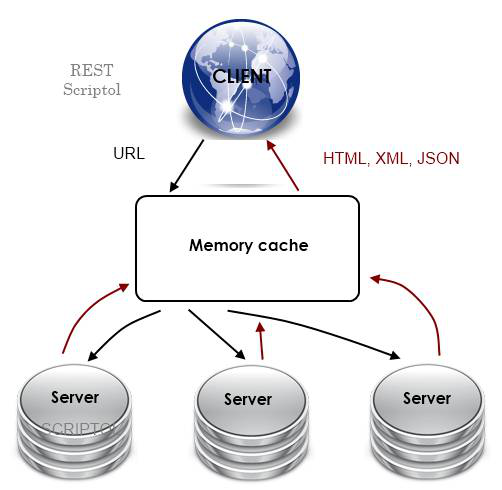
\includegraphics[scale=0.7]{imgs/rest_architecture.png} 
\caption{Modello di architettura REST\label{restimage}}
\end{center}
\end{figure}
\\
Un numero qualsiasi di connettori (client, server, cache, tunnel ecc.) può mediare la richiesta, ma ogni connettore interviene senza conoscere la “storia passata” delle altre richieste(stateless). Di conseguenza una applicazione può interagire con una risorsa conoscendo due cose: l'identificatore della risorsa e l'azione richiesta.
L'applicazione deve conoscere il formato dell'informazione (rappresentazione) restituita, tipicamente un documento HTML, XML o JSON, ma potrebbe essere anche un'immagine o qualsiasi altro contenuto.

\subsubsection{Scelte}

\clearpage{\pagestyle{empty}\cleardoublepage}

\section{Tecnologie di Sviluppo}
\subsection{.NET Framework}
Il \textbf{.NET Framework} è un software framework sviluppato da Microsoft che gira principalmente su sistema operativo Microsoft Windows.
Include una vasta libreria e fornisce interoperabilità di linguaggio attraverso diversi linguaggi di programmazione.
I programmi scritti per il il .NET Framework sono eseguiti in un ambiente software, conosciuto come \emph{Common Language Runtime}, una macchina virtuale che fornisce servizi come sicurezza, gestione della memoria e delle eccezioni.
La libreria delle classi e il Common Language Runtime costituiscono insieme il .NET Framework.
La Base Class Library del .NET Framework fornisce interfacce utente, accesso ai dati, connettività al database, crittografia, sviluppo di applicazioni web, algoritmi numerici e comunicazioni di rete.
I programmatori producono software combinando codice sorgente con .NET Framework e altre librerie.
Microsoft fornisce, inoltre, un ambiente di sviluppo integrato per il software .NET chiamato \emph{Visual Studio}.

Nell'agosto 2012, è stato rilasciato il \emph{.NET Framework 4.5}.

\subsubsection{Design}
Le caratteristiche di design del .NET Framework sono:
\begin{itemize}
\item \emph{Interoperabilità}: .Net Framework fornisce strumenti per accedere a funzionalità implementate in programmi più o meno recenti che sono eseguiti al di fuori dell'ambiente .NET, al fine di favorire l'interazione tra applicazioni;
\item \emph{Common Language Runtime}: serve come motore per eseguire il framework .NET. Tutti i programmi .NET sono eseguiti sotto la supervisione del CLR, garantendo proprietà e comportamenti definiti riguardo sicurezza, memoria e gestione delle eccezioni;
\item \emph{Indipendenza dal linguaggio}: E' introdotto il \emph{Common Type System} o CTS, che specifica tutti i possibili tipi di dati e costrutti di programmmazione supportati dal CLR e come essi possano o meno interagire con gli altri attraverso le specifiche del \item \emph{Common Language Infrastructure};
\item \emph{Base Class Library}: fornisce classi che incapsulano un gran numero di funzioni comuni, come creazione di interfacce utente, accesso ai file, rendering grafico, manipolazione documenti XML, connettività al database, crittografia, sviluppo di applicazioni web, algoritmi numerici e comunicazioni di rete. E' disponibile per tutti i linguaggi che utilizzano il .NET Framework;
\item \emph{Rilascio semplificato}: sono presenti tool che facilitano l'installazione del software sviluppato e assicurano che quest'ultimo non interferisca con software preinstallato e che sia conforme ai requisiti di sicurezza;
\item \emph{Sicurezza}: è fornito un modello di sicurezza comune per tutte le applicazioni, oltre a meccanismi di protezione da vari tipi di vulnerabilità;
\item \emph{Portabilità}: il framework .NET è \emph{platform-agnostic} e sono disponibili implementazioni multipiattaforma per altri sistemi operativi. Il Common Language Infrastructure, ilinguaggi C\# e C++ sono tutti standard ECMA e ISO. Questo rende possibile la creazione di implementazioni compatibili col framework da terze parti.
\end{itemize}


\subsubsection{Architettura}
Il .NET Framework è costituito da:
\begin{itemize}
\item \emph{Common Language Infrastructure};
\item \emph{Sicurezza};
\item \emph{Librerie di classi};
\item \emph{Gestione della memoria}.
\end{itemize}
che di seguito sono brevemente introdotti.
\paragraph{Common Language Infrastructure}
CLI fornisce una piattaforma neutra per lo sviluppo e l'esecuzione delle applicazioni. Tale piattaforma include funzioni per la gestione delle eccezioni, la \emph{garbage collection}, la sicurezza e l'interoperabilità.
\begin{figure}
\begin{center}
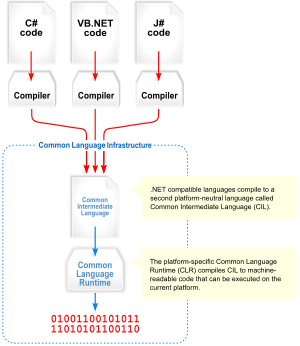
\includegraphics[scale=0.4]{imgs/commonlanguageinfrastructure.png} 
\caption{Panoramica della Common Language Infrastructure\label{commonlanguageinfrastructure}}
\end{center}
\end{figure}
Siccome gli aspetti basilari del .NET Framework sono stati implementati nell'ambito di CLI, questa funzionalità non è legata ad un singolo linguaggio ma è disponibile a tutti i linguaggi supportati dal framework.
Il codice CLI è contenuto in file assembly, conservati in formato \emph{Portable Executable} PE, comune alla piattaforma windows per tutti i file DLL e EXE.
L'assembly consiste in uno o più file, uno dei quali contiene il manifest, che rappresenta il metadato dell'assembly.
Il nome completo di un assembly contiene nome, numero di versione, \emph{culture} e chiave pubblica, quindi se due assembly hanno lo stesso nome completo, essi sono considerati uguali.



%The CIL code is housed in CLI assemblies. As mandated by the specification, assemblies are stored in the Portable Executable (PE) format, common on the Windows platform for all DLL and EXE files. The assembly consists of one or more files, one of which must contain the manifest, which has the metadata for the assembly. The complete name of an assembly (not to be confused with the filename on disk) contains its simple text name, version number, culture, and public key token. Assemblies are considered equivalent if they share the same complete name, excluding the revision of the version number. A private key can also be used by the creator of the assembly for strong naming. The public key token identifies which public key an assembly is signed with. Only the creator of the keypair (typically the .NET developer signing the assembly) can sign assemblies that have the same strong name as a previous version assembly, since he is in possession of the private key. Strong naming is required to add assemblies to the Global Assembly Cache

\paragraph{Sicurezza}
Il Framework .NET ha meccanismi propri di security con due caratteristiche fondamentali: Code Access Security (CAS) e validazione e verifica.
Code Access Security è basato su un \emph{evidenza} che è associata con uno specifico assembly. Tipicamente l'evidenza è la sorgente dell'assembly(qualora sia stato installato sulla macchina locale o sia stato scaricato dalla rete).
Code Access Security usa l'evidenza per determinare le autorizzazioni concesse al codice.
Altre porzioni di codice possono chiedere se al codice chiamante sono concesse specifiche autorizzazioni; in tal caso, il CLR esegue un controllo allo stack ed ogni metodo presente nello stack viene controllato sulle autorizzazioni richieste. Se nessun assembly concede l'autorizzazionie, viene lanciata un'eccezione sulla sicurezza.
 
\paragraph{Librerie di classi}
Il Framework .NET include un insieme di librerie standard, organizzate in  gerarchie di namespaces. La maggior parte delle API presenti sono parti dei namespaces \emph{System.*} o \emph{Microsoft.*} e implementano un gran numero di funzionalità comuni come, tra le altre, la lettura e la scrittura su file, il rendering grafico, l'interazione con i database e la manipolazione dei file XML.
Le librerie sono divise in due macrocategorie: la Base Class Library e la Framework Class Library.
La Base Class Library include un piccolo insieme dell'intera libreria ma contiene le API di base del Common Language Runtime.
La Framework Class Library contiene la Base Class Library e si riferisce all'intera classe di librerie .NET, includendo, tra le altre, Windows Forms, ADO.NET, ASP.NET, Language Integrated Query (LINQ), Windows Presentation Foundation, Windows Communication Foundation.
\paragraph{Gestione della memoria}
Il Framework .NET libera lo sviluppatore dalla necessità di gestire l'allocazione e la deallocazione della memoria, dal momento che è presente un sistema che controlla quando la memoria può essere liberata in sicurezza. Le instanze degli oggetti .NET sono allocate nello heap, un pool di memoria gestito dal CLR. Quando ci sono riferimenti a quell'oggetto, esso è considerato in uso, ma, quando i riferimenti non ci sono più, l'oggetto non è più raggiungibile e quindi viene cancellato.
Il .NET Garbage Collector viene eseguito periodicamente, su un thread separato da quello dell'applicazione, solamente quando una definita quantità di memoria è stata utilizzata o c'è un alto utilizzo di memoria di sistema.

%The .NET Garbage Collector (GC) is a non-deterministic, compacting, mark-and-sweep garbage collector. The GC runs only when a certain amount of memory has been used or there is enough pressure for memory on the system. Since it is not guaranteed when the conditions to reclaim memory are reached, the GC runs are non-deterministic. Each .NET application has a set of roots, which are pointers to objects on the managed heap (managed objects). These include references to static objects and objects defined as local variables or method parameters currently in scope, as well as objects referred to by CPU registers.[10] When the GC runs, it pauses the application, and for each object referred to in the root, it recursively enumerates all the objects reachable from the root objects and marks them as reachable. It uses CLI metadata and reflection to discover the objects encapsulated by an object, and then recursively walk them. It then enumerates all the objects on the heap (which were initially allocated contiguously) using reflection. All objects not marked as reachable are garbage.[10] This is the mark phase.[11] Since the memory held by garbage is not of any consequence, it is considered free space. However, this leaves chunks of free space between objects which were initially contiguous. The objects are then compacted together to make used memory contiguous again.[10][11] Any reference to an object invalidated by moving the object is updated by the GC to reflect the new location.[11] The application is resumed after the garbage collection is over.
%The GC used by .NET Framework is also generational.[12] Objects are assigned a generation; newly created objects belong to Generation 0. The objects that survive a garbage collection are tagged as Generation 1, and the Generation 1 objects that survive another collection are Generation 2 objects. The .NET Framework uses up to Generation 2 objects.[12] Higher generation objects are garbage collected less frequently than lower generation objects. This helps increase the efficiency of garbage collection, as older objects tend to have a longer lifetime than newer objects.[12] Thus, by eliminating older (and thus more likely to survive a collection) objects from the scope of a collection run, fewer objects need to be checked and compacted.[12]



\subsubsection{Microsoft Visual Studio}
Microsoft Visual Studio (\emph{\url{http://www.microsoft.com/visualstudio/ita}}), rappresentata con uno screenshot in figura \ref{vsimage}, permette lo sviluppo di applicazioni console, siti internet, applicazioni grafiche, applicazioni e servizi web, librerie di classi, servizi Windows in tutti i linguaggi di programmazione supportati dal framework .NET, oltre che in tutti i linguaggi di markup, JavaScript e CSS.

\begin{figure}
\begin{center}

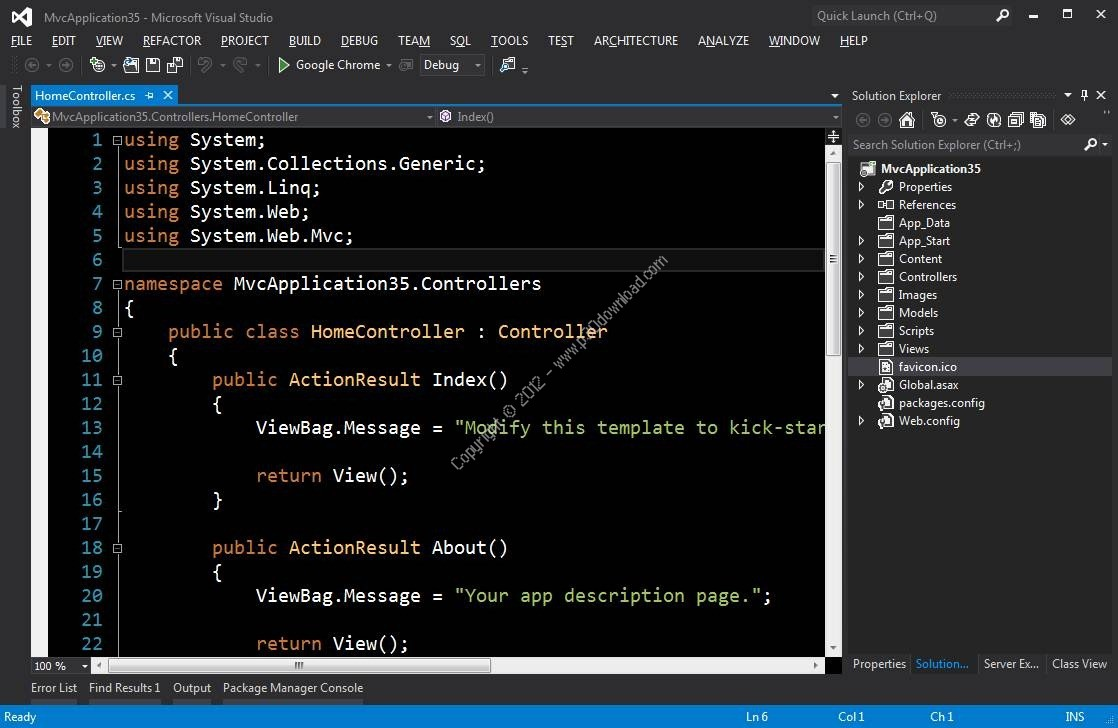
\includegraphics[scale=0.3]{imgs/visualstudio.jpg} 
\caption{Schermata di Visual Studio 2012 Ultimate\label{vsimage}}
\end{center}

\end{figure}
Visual Studio fornisce all’utilizzatore un potente strumento, \textbf{IntelliSense}, che permette
l'autocompletamento del token che il programmatore intende scrivere, oltre che
alla visualizzazione della documentazione e alla gestione delle disambiguità a
video direttamente durante la scrittura del codice.

La versione utilizzata è \textbf{Visual Studio 2013}, lanciata nel giugno 2013.
Essa fornisce numerose nuove features, brevemente elencate:
\begin{itemize}
\item \textbf{Colorazione semantica}: è stata migliorata la colorazione della sintassi, compresi i tipi definiti dall'utente, le macro, i tipi enumerativi e le funzioni;
\item \textbf{Evidenziazione dei riferimenti}: selezione di tutti i riferimenti di un simbolo, una volta selezionato quest'ultimo;
\item \textbf{Nuovo Solution Explorer}: il nuovo Solution Explorer consente agli utenti una visualizzazione per classi o gerarchie di file all'interno del progetto.
E' supportata inoltre la ricerca di chiamate ad una funzione ed utilizzo delle classi;
\item \textbf{Visualizzazione automatica della lista IntelliSense}: IntelliSense è automaticamente visualizzato mentre viene scritto il codice;
\item \textbf{Filtraggio della lista degli elementi}: IntelliSense usa una \textit{fuzzy logic} per determinare quali funzioni/variabili/tipi visualizzare nella lista;
\item \textbf{Code snippets}: è incluso in Intellisense per generare automaticamente frammenti di codice basati sui parametri dell'utente.
\end{itemize}

\subsubsection{TFS - Team Foundation Service}
Visual Studio offre, tra i vari servizi, \textbf{Team Foundation Service}, uno strumento di gestione collaborativa del codice che consente di:
\begin{itemize}
\item controllare il proprio codice direttamente in \textit{cloud}, rendendolo accessibile ovunque;
\item gestire il versioning del progetto;
\item gestire la collaborazione nel team;
\item pianificare lo sviluppo agile;
\item gestire il testing e la distribuzione del prodotto.
\end{itemize}

\clearpage{\pagestyle{empty}\cleardoublepage}

\subsection{Metodologia agile}
Con il termine \textit{metodologia agile} si intende un insieme di metodi di sviluppo software basati sullo sviluppo iterativo ed incrementale, in cui i requisiti e le soluzioni evolvono attraverso una collaborazione tra team capaci di organizzarsi autonomamente e con esperienze e conoscenze diverse.
Le metodologie agili sono contrapposte alle metodologie \textit{pesanti} e \textit{iterative} poiché promuovono una pianificazione adattabile, uno sviluppo e una consegna del software evolutivi, un approccio iterativo, ed incoraggiano ad una risposta al cambiamento rapida e flessibile.

Le metodologie agili sono state introdotte ufficialmente nel 2001 dal \textit{Manifesto Agile}(\url{http://agilemanifesto.org/}), un documento dell'\textit{Agile Alliance}, l'associazione che ha permesso la diffusione su ampia scala di tali metodologie.
Il Manifesto Agile riporta quanto segue:
\begin{quotation}
\begin{emph}
We are uncovering better ways of developing software by doing it and helping others do it. Through this work we have come to value:
\begin{itemize}
\item[ ] Individuals and interactions over processes and tools
\item[ ] Working software over comprehensive documentation
\item[ ] Customer collaboration over contract negotiation
\item[ ] Responding to change over following a plan
\end{itemize}
That is, while there is value in the items on the right, we value the items on the left more.
\end{emph}
\end{quotation}
I metodi agili quindi preferiscono la comunicazione in tempo reale, preferibilmente faccia a faccia, a quella scritta (documentazione). Il team agile è composto da tutte le persone necessarie per terminare il progetto software. Come minimo il team deve includere i programmatori ed i loro clienti. (Con clienti si intendono le persone che definiscono come il prodotto dovrà essere fatto. Possono essere dei Product Manager, dei Business Analysts, o i clienti finali). L'obiettivo è la piena soddisfazione del cliente e non solo l'adempimento di un contratto. 
L'uso di queste metodologia, inoltre, serve ad abbattere i costi di sviluppo del software e a ridurre al minimo la parte di progettazione che spesso era quella più dispendiosa. Essa è esplosa proprio in concomitanza con la crisi successiva al boom di Internet prendendo spunto dai metodi applicati in piccole software house. Sotto questo nome si raggruppano tecniche come Extreme Programming, SCRUM, Feature Driven Development, DSDM, Disciplined Agile Delivery, Crystal e Lean Software Development.

\subsubsection{Processi di sviluppo agile}
Così come per i processi di sviluppo tradizionali, anche durante lo sviluppo di software mediante metodologie agili, ci sono delle fasi predefinite: analisi dei requisiti, progettazione, sviluppo e testing. La differenza è che ad ogni iterazione lo sviluppatore ridefinisce e rielabora queste fasi.
I requisiti sono, ad ogni iterazione, approfonditi e migliorati, così come è perfezionato il design. Inoltre è dato molta importanza alla rifattorizzazione, ovvero si modifica la struttura interna di porzioni di codice senza modificarne il comportamento esterno, così da migliorarne la leggibilità ed avere sempre codice di qualità.
Il testing, nell'Agile, riveste un ruolo fondamentale, poiché sono previsti sia gli \textit{Acceptance Test}, ovvero test \textbf{black box} che rappresentano dei risultati attesi dal sistema.
Inoltre vi è il Test Driven Development (TDD), ovvero un modello di sviluppo preceduto dalla stesura di test automatici.

In figura \ref{agiledevelopment} vi è una rappresentazione del processo di sviluppo agile.

\begin{figure}[h!]
\begin{center}
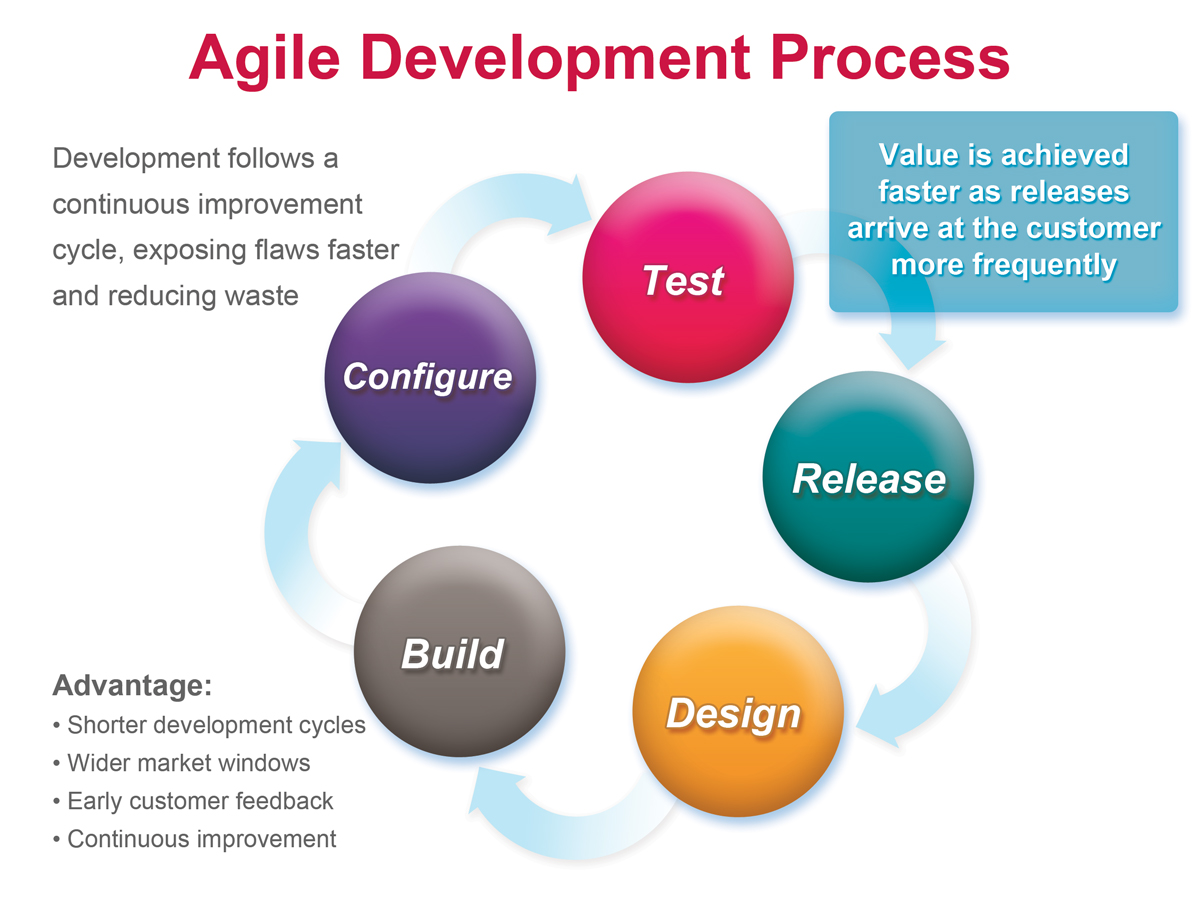
\includegraphics[scale=0.27]{imgs/agiledevelopment.jpg}
\caption{Processo di sviluppo agile\label{agiledevelopment}} 
\end{center}
\end{figure}

La gran parte dei metodi agili tenta di ridurre il rischio di fallimento sia in termini economici, poiché si ha la possibilità di stabilire un tetto di spese limitate che è negoziato frequentemente e monitorato su base costante, sia inteso come forte riduzione del rischio che il cliente si ritrovi in mano funzionalità che non utilizzerà mai o molto raramente. Tutto ciò si può ottenere sviluppando il software in finestre di tempo limitate chiamate \textit{iterazioni} che, in genere, durano qualche settimana.
I fondamenti dei processi agili sono i seguenti:
\begin{itemize}
\item \textbf{iteratività}: prescrive che il processo di sviluppo debba essere ciclico, in modo che le varie fasi siano ripetute più volte in momenti temporali diversi. Questo permette di gestire in modo agile i cambiamenti delle specifiche durante il processo, e non costringe ad aspettare il rilascio del prodotto per poi intraprendere subito una fase di manutenzione, come invece accade con i metodi tradizionali;
\item \textbf{incrementalità}: è il continuo rilascio di versioni parziali del prodotto, le quali inglobano modifiche ed aggiornamenti risultati come necessari alle fasi precedenti. Questo meccanismo permette di rilevare i feedback del committente durante il processo di sviluppo e di adeguare opportunamente il software. In alcuni casi il software rilasciato nelle fasi intermedie è sottoposto anche agli utenti finali, in modo da coglierne le esigenze;
\item \textbf{auto-organizzazione}: il team è lasciato libero di organizzarsi e di adottare di volta in volta le strategie più opportune. Questo favorisce la creatività degli sviluppatori, stimolandoli a trovare soluzioni innovative ai problemi che si presentano;
\item \textbf{emergenza}: bisogna affrontare difficoltà ed imprevisti quando essi si presentano, senza cercare di predeterminarli o una prevenirli. Il principio tradizionale secondo cui un progetto solido deve tener conto dei possibili sviluppi futuri del software viene sovvertito, con la motivazione che si considera inutile spendere tempo e denaro per cercare di prevedere evoluzioni che potrebbero essere disattese.
\end{itemize}





%%%%\clearpage{\pagestyle{empty}\cleardoublepage}
%%%%%%%%%%%%%%%%%%%%%%%%%%%%%%%%%%%%%%%%%%%%%%%%%%%%%%%%%%%

\chapter{Realizzazione}
\label{ref:realizzazione}

In questo capitolo verrà discussa l'effettiva realizzazione del progetto, ovvero analisi dei requisiti, progettazione, sviluppo e testing, secondo le metodologie agili.
Ogni progetto inizia con la stesura di un \textit{Project Charter} (Documento di inizio progetto), che, non essendo di interesse in questo contesto, viene qui tralasciato.
Si è proceduto quindi con la definizione delle iterazioni, partendo, naturalmente, dall'\textit{iterazione 0}

\section{Iterazione 0}

Nell'\emph{iterazione 0}, come prassi nelle metodologie agili, vengono realizzate l'analisi dei requisiti, la modellazione delle interfacce utente, la modellazione di dominio e la pianificazione degli incrementi.
L'\emph{iterazione 0} è la base su cui partire per lo sviluppo delle iterazioni successive, perciò ricopre un ruolo fondamentale nello sviluppo Agile.

\subsection{Analisi dei requisiti}
Di seguito sono descritti i requisiti funzionali e non funzionali.

\subsubsection{Requisiti funzionali}
I requisiti funzionali descrivono le funzionalità del sistema software, in termini di servizi che il sistema software deve fornire, di come il sistema software reagisce a specifici tipi di input e di come si comporta in situazioni particolari.
Qui, i requisiti funzionali vengono descritti sotto forma di \textit{user stories}, \textit{epic} (user stories più grandi) e \textit{temi}.

Durante l'analisi è stato individuato un unico tema comune, ovvero:
\begin{itemize}
\item \textit{Gestisci la navigazione assistita del sito}.
\end{itemize}

Da questo tema possiamo ricavare tre \textit{epic}:
\begin{itemize}
\item \textit{Gestisci la mappa del sito};
\item \textit{Gestisci i punti di interesse del sito};
\item \textit{Gestisci l'itinerario del sito}.
\end{itemize}.

Ed, in definitiva, da questi tre epic, possiamo ricavare otto \textit{user stories} che caratterizzano i requisiti dell'applicazione. Tali user stories vengono di seguito riportate, secondo il formato \emph{"essendo un\dots vorrei poter\dots così da\dots"}, comunemente utilizzato:

\begin{itemize}
\item \textit{essendo un utente vorrei poter visualizzare la mia posizione sulla mappa così da orientarmi al meglio all'interno del sito};
\item \textit{essendo un utente vorrei poter visualizzare i punti di interesse sulla mappa così da spostarmi verso di essi};
\item \textit{essendo un utente vorrei poter zoomare e centrare la mappa così da ottenere una visualizzazione migliore};
\item \textit{essendo un utente vorrei poter sapere quando sono vicino ad un punto di interesse così da conoscere informazioni su di esso};
\item \textit{essendo un utente vorrei poter cliccare su un punto di interesse così da conoscere informazioni su di esso};
\item \textit{essendo un utente vorrei poter conoscere i feedback degli altri utenti così da spostarmi verso punti di interesse dal rating noto};
\item \textit{essendo un utente vorrei poter inviare un feedback così da condividere la mia esperienza con gli altri utenti};
\item \textit{essendo un utente vorrei poter ottenere un itinerario così da ottimizzare il tempo di visita}.
\end{itemize}


Per quanto riguarda il servizio, esso deve fornire un file in formato GeoRSS contenente i punti di interesse con le informazioni fondamentali (nome, coordinate spaziali, feedback).

\subsubsection{Requisiti non funzionali}
I requisiti non funzionali descrivono le proprietà del sistema software in relazione a determinati servizi o funzioni e possono anche essere relativi al processo:
\begin{itemize}
\item caratteristiche di efficienza, affidabilità, safety, ecc\dots;
\item caratteristiche del processo di sviluppo (standard di processo, uso di ambienti CASE, linguaggi di programmazione, metodi di sviluppo, ecc\dots);
\item caratteristiche esterne (interoperabilità con sistemi di altre organizzazioni, vincoli legislativi, ecc\dots).
\end{itemize}

Nel caso di sistemi software destinati a dispositivi mobili, vengono introdotte nuove criticità e nuove proprietà da tenere in considerazione che possono essere riassunte in:
\begin{itemize}
\item \textbf{prestazioni}: i dispositivi mobile hanno risorse limitate, in termini di memoria e di potenza di calcolo, per cui le applicazioni devono poter essere eseguite abbastanza efficientemente;
\item \textbf{usabilità}: i dispositivi mobile presentano display dalle dimensioni ridotte, per cui deve essere posta particolare attenzione al design dell'interfaccia;
\item \textbf{funzionalità}: i dispositivi mobile possono avere diverse periferiche (WIFI, GPS, camera), per cui le applicazioni devono tener conto di queste periferiche e bisogna definire il comportamento di esse in caso non fossero presenti tali periferiche;
\item \textbf{connettività}: i dispositivi mobile, in alcune circostanze, possono non avere caratteristiche di connettività (assenza segnale GPS, UMTS o HDSPA, etc\dots) per cui è importante definire il comportamento dell'applicazione in questi casi;
\item \textbf{consumi}:i dispositivi mobile, in quanto alimentati da batterie, sono soggetti a un consumo che dipende anche dalle periferiche utilizzate (WIFI, GPS, flash fotografico, etc\dots).
\end{itemize}

Nello studio dei requisiti della nostra applicazione, si possono definire i requisiti non funzionali di alto livello dell'applicazione client e del server, descritti rispettivamente nelle tabelle in figura \ref{nfrclient} e \ref{nfrserver}.

\begin{figure}[h!]
\begin{center}
\begin{tabular}[c]{|c|p{9cm}|}
\hline
N. & Requisito\\ \hline
1 & L'interfaccia deve essere costituita da una mappa e da una barra di pulsanti\\ \hline
2 & L'applicazione deve impiegare al massimo 10 secondi per l'avvio\\ \hline
3 & L'applicazione deve utilizzare le periferiche disponibili solo quando necessario\\ \hline
4 & L'applicazione deve funzionare con una risoluzione minima di 480x800\\ \hline
5 & L'applicazione deve prevedere una modalità Offline quando non c'è connettività\\ \hline
\end{tabular}
\caption{Requisiti non funzionali dell'applicazione client\label{nfrclient}}
\end{center}
\end{figure}
\begin{figure}[h!]
\begin{center}
\begin{tabular}[c]{|c|p{9cm}|}
\hline
N. & Requisito\\ \hline
1 & Il servizio deve poter funzionare con almeno 10 richieste al secondo\\ \hline
2 & Il servizio deve essere sempre disponibile almeno negli orari di visita del sito\\ \hline
3 & Il servizio deve essere accessibile esclusivamente dai client dell'applicazione\\ \hline
\end{tabular}
\caption{Requisiti non funzionali del server\label{nfrserver}}
\end{center}
\end{figure}


\subsection{Modello di dominio}
Il modello di dominio identifica le entità fondamentali e le relazioni tra esse.
Sono state individuate cinque entità fondamentali:
\begin{itemize}
\item \textbf{Utente}: è la classe che rappresenta l'utilizzatore dell'applicazione. Collabora con le classi Posizione, Feedback;
\item \textbf{Punto di interesse}: è la classe che rappresenta tutte le strutture, i monumenti e le opere d'arte. Ha come caratteristiche intrinseche il nome, un'icona e una url. Collabora con le classi Posizione e Feedback;
\item \textbf{Posizione}: è la classe che definisce il posizionamento di un punto di interesse, in termini di latitudine e longitudine;
\item \textbf{Feedback}: è la classe che definisce il giudizio dato dall'utente. Ha come caratteristiche il voto (in termini numerici), il giudizio e la data;
\item \textbf{Itinerario}: è la classe responsabile di gestire i percorsi. Collabora con la classe Punto di interesse.
\end{itemize}
\begin{figure}
\begin{center}
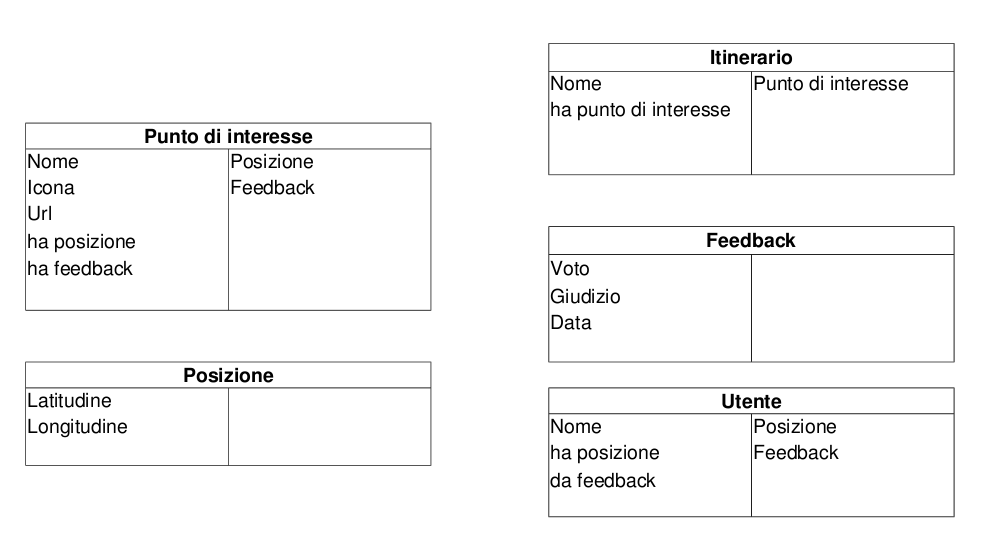
\includegraphics[scale=0.50]{imgs/model/crcmodel.png}
\caption{Modello CRC dell'applicazione\label{crcmodel}}
\end{center}
\end{figure}
Per modellare il dominio vengono qui utilizzate le \textit{Class Responsibility Collaborator (CRC) Cards}, come illustrato in figura \ref{crcmodel}.

\subsection{Modello dell'interfaccia utente}
L'interfaccia utente è la porzione di software che interagisce direttamente con l'utente.
In base ai requisiti non funzionali che caratterizzano l'interfaccia utente, si cerca di realizzare interfacce che tengano conto dell'usabilità.
Vengono riportati di seguito alcuni sketches che costituiscono le schermate dell'applicazione (fig. \ref{sketch}).
\begin{figure}[h!]
\subfloat[Home]{\label{mockuphome}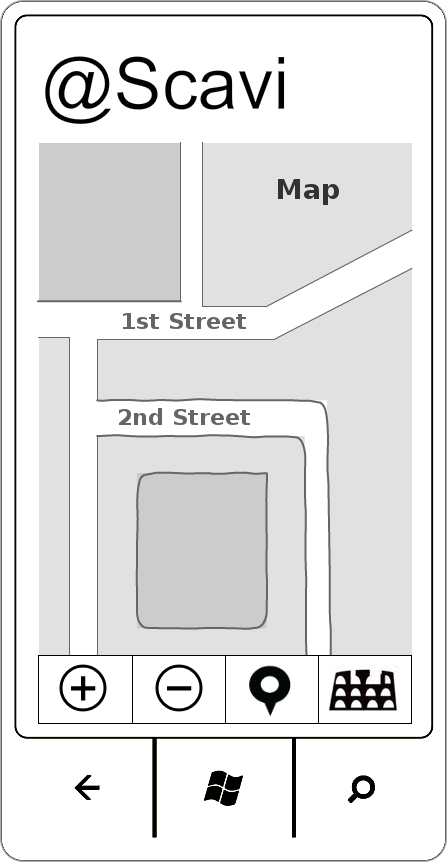
\includegraphics[scale=0.29]{imgs/mockup/home.png}}
\hspace{35mm}
\subfloat[Visualizzazione posizione]{\label{mockupposition}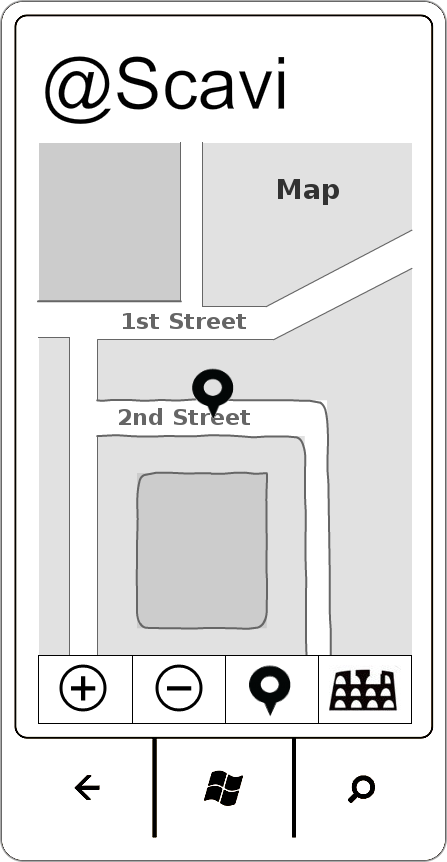
\includegraphics[scale=0.29]{imgs/mockup/position.png}}
 \hspace{35mm}
\subfloat[Visualizzazione punti di interesse]{\label{mockuppushpin}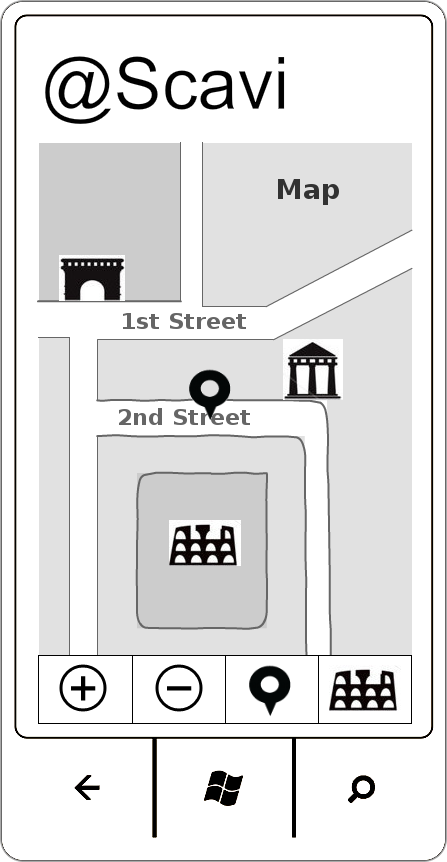
\includegraphics[scale=0.29]{imgs/mockup/pushpin.png}}
 \hspace{35mm}
\subfloat[Visualizzazione menu]{\label{mockuptooltipmenu}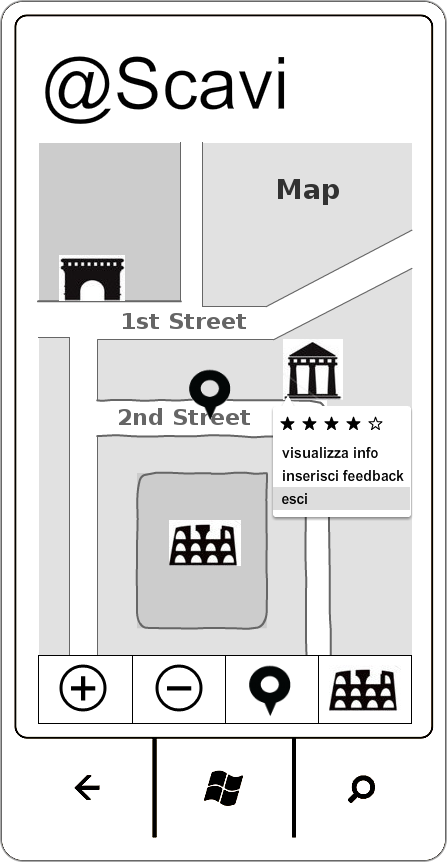
\includegraphics[scale=0.29]{imgs/mockup/tooltipmenu.png}} 
 \hspace{35mm}

\caption{Sketch dell'applicazione, 1\label{sketch}}
\end{figure}

\begin{figure}[h!]
\ContinuedFloat 
\subfloat[Visualizzazione dettaglio]{\label{mockupdetails}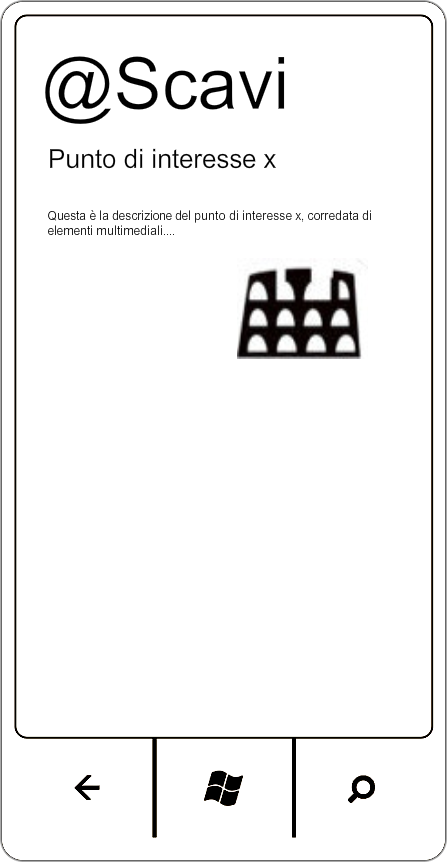
\includegraphics[scale=0.29]{imgs/mockup/details.png}}
 \hspace{35mm}
\subfloat[Invio feedback]{\label{mockupsendfeedback}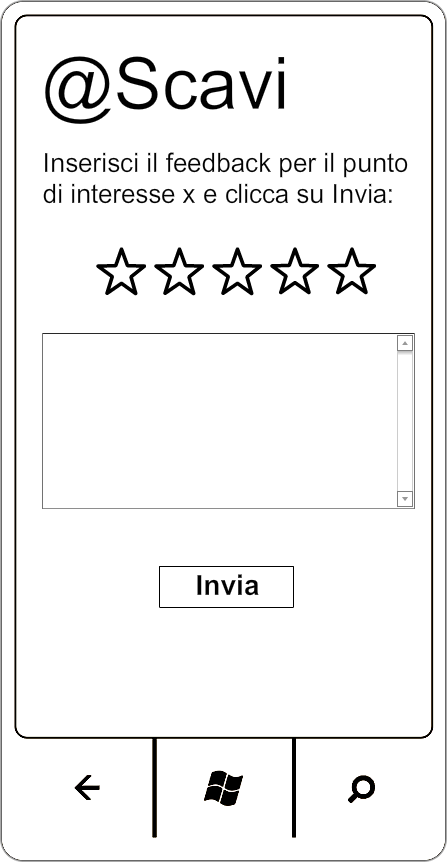
\includegraphics[scale=0.29]{imgs/mockup/sendfeedback.png}}
 \hspace{35mm}

\subfloat[Itinerario]{\label{mockupitinerario}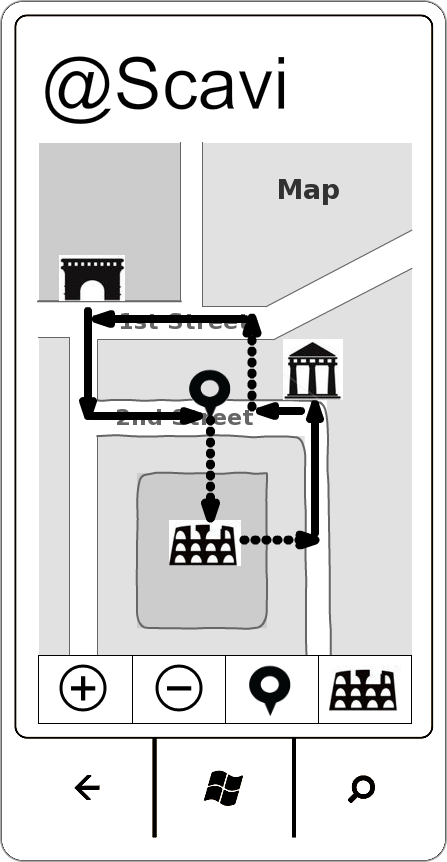
\includegraphics[scale=0.29]{imgs/mockup/route.png}}

\caption{Sketch dell'applicazione, 2\label{sketch}}
\end{figure}

%\Image[width=0.35\linewidth]{imgs/mockup/home.png}{Home}\,
%\Image[width=0.35\linewidth]{imgs/mockup/position.png}{Visualizzazione posizione}
%
%\Image[width=0.35\linewidth]{imgs/mockup/pushpin.png}{Visualizzazione punti di interesse}\,
%\Image[width=0.35\linewidth]{imgs/mockup/tooltipmenu.png}{Visualizzazione menu contestuale}
%
%\Image[width=0.35\linewidth]{imgs/mockup/details.png}{Visualizzazione dettagli} \,
%\Image[width=0.35\linewidth]{imgs/mockup/sendfeedback.png}{Invio feedback}
%
%\Image[width=0.35\linewidth]{imgs/mockup/route.png}{Itinerario}
%\captionof{figure}{Sketch dell'applicazione\label{sketch}}
\clearpage

\subsection{Pianificazione degli incrementi}
Tramite il planning poker\footnote{Il planning poker è una tecnica basata sul consenso per stimare lo sforzo nel completare una user story. E' largamente utilizzata in nelle metodologie agili.}, è stato possibile dare una stima della complessità delle user stories.

\begin{figure}[h!]
\begin{center}
\begin{tabular}[c]{|c|p{7cm}|c|c|}
\hline
N. & User story & Peso & Priorità\\
\hline
1 & \textit{essendo un utente vorrei poter visualizzare la mia posizione sulla mappa così da orientarmi meglio all'interno del sito} & 5 & 10\\
\hline
2 & \textit{essendo un utente vorrei poter visualizzare i punti di interesse sulla mappa così da spostarmi verso di essi} & 8 & 10\\
\hline
3 & \textit{essendo un utente vorrei poter zoomare e centrare la mappa così da ottenere una visualizzazione migliore} & 3 & 9\\
\hline
4 & \textit{essendo un utente vorrei poter sapere quando sono vicino ad un punto di interesse così da conoscere informazioni su di esso} & 5 & 8\\
\hline
5 & \textit{essendo un utente vorrei poter cliccare su un punto di interesse così da conoscere informazioni su di esso} & 3 & 7\\
\hline
6 & \textit{essendo un utente vorrei poter conoscere i feedback degli altri utenti così da spostarmi verso punti di interesse dal rating noto} & 3 & 6\\
\hline
7 & \textit{essendo un utente vorrei poter inviare un feedback così da condividere la mia esperienza con gli altri utenti} & 5 & 5\\
\hline
8 & \textit{essendo un utente vorrei poter ottenere un itinerario così da ottimizzare il tempo di visita} & 15 & 5\\
\hline
\end{tabular}
\caption{Tabella di stima delle user stories\label{userstoriestable}}
\end{center}
\end{figure}
\clearpage

In definitiva abbiamo la tabella in figura \ref{userstoriestable}, con stima e priorità delle user stories.
Considerando una velocità di 15 punti per iterazione e tenendo conto delle priorità, è stato possibile pianificare 3 iterazioni, ciascuna della durata di due settimane, come illustrato in figura \ref{pianificazioneiterazioni}.
Quindi, il progetto verrà sviluppato in sei settimane.
\begin{figure}[h!]
\begin{center}

\begin{tabular}[c]{|c|p{7cm}|c|c|}
\hline
Iterazione & User story\\ \hline
\textbf{Prima iterazione} & 1,2,3 \\ \hline
\textbf{Seconda iterazione} & 4,5,6,7\\ \hline
\textbf{Terza iterazione} & 8\\ \hline
\end{tabular}
\caption{Pianificazione delle iterazioni\label{pianificazioneiterazioni}}

\end{center}
\end{figure}

\clearpage

\section{Iterazione 1}
Nelle iterazione 1 viene effettuata l'analisi dei requisiti per tutti i requisiti corrispondenti alle user stories che ne fanno parte; vengono esplicitati i casi di test; vengono sviluppati alcuni modelli, in particolare i modelli strutturali (modello dei dati e diagramma delle classi) e i modelli comportamentali (diagramma di sequenza), migliorando e ridefinendo, se necessario, i modelli dell'iterazione precedente; vengono, inoltre, mostrati alcuni dettagli di implementazione corrispondenti a porzioni di codice; infine vengono mostrati gli screenshot dell'applicazione.\\

\subsection{Analisi dei Requisiti}
Nell'analisi dei requisiti, le \textit{user stories} vengono suddivise in task; i requisiti non funzionali vengono validati, migliorati e approfonditi.

%Gli sketch della prima iterazione sono quelli in figura \ref{sketch1iterazione}.
%\begin{figure}
%\subfigure[prima]{ 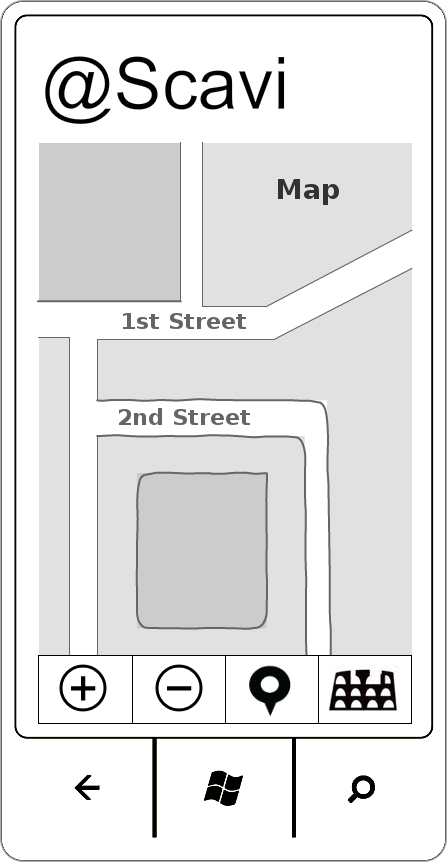
\includegraphics[scale=0.29]{imgs/mockup/home.png} }
%\subfigure[seconda]{ 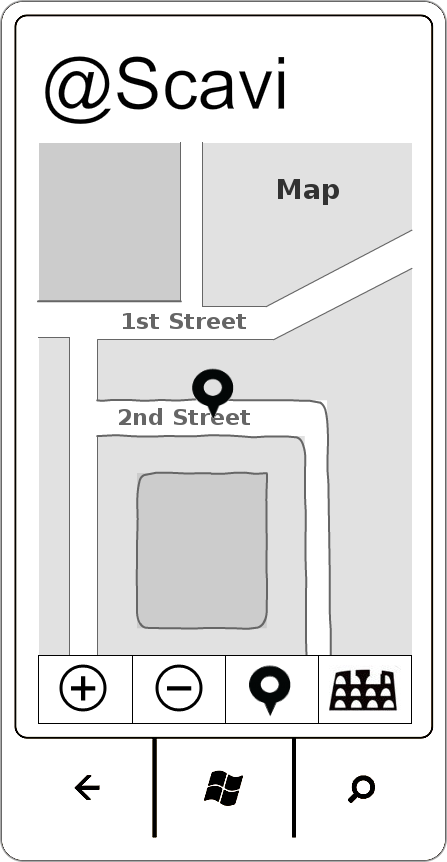
\includegraphics[scale=0.29]{imgs/mockup/position.png} }
%\subfigure[terza]{ 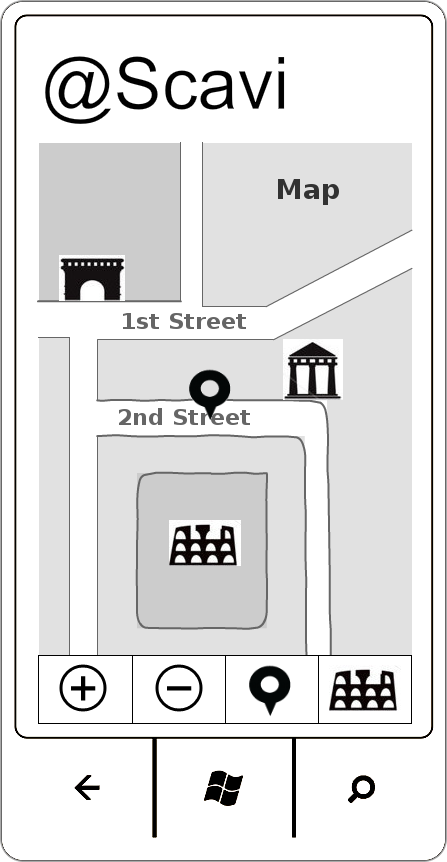
\includegraphics[scale=0.29]{imgs/mockup/pushpin.png} }
%\caption{Sketch della prima iterazione, I\label{sketch1iterazione}}
%\end{figure}
\subsubsection{Requisiti funzionali}
In questa iterazione, come già specificato prima, sono sviluppate le user stories 1,2 e 3 (fig. \ref{userstoriestableprimaiterazione}). \\
\begin{figure}[h!]
\begin{center}
\begin{tabular}[c]{|c|p{7cm}|c|c|}
\hline
N. & User story & Peso & Priorità\\
\hline
1 & \textit{essendo un utente vorrei poter visualizzare la mia posizione sulla mappa così da orientarmi meglio all'interno del sito} & 5 & 10\\
\hline
2 & \textit{essendo un utente vorrei poter visualizzare i punti di interesse sulla mappa così da spostarmi verso di essi} & 8 & 10\\
\hline
3 & \textit{essendo un utente vorrei poter zoomare e centrare la mappa così da ottenere una visualizzazione migliore} & 3 & 9\\
\hline
\end{tabular}
\caption{Tabella di stima delle user stories della prima iterazione\label{userstoriestableprimaiterazione}}
\end{center}
\end{figure}
\clearpage

Considerando le tre user stories, possiamo definire i seguenti task che caratterizzeranno la prima iterazione:\\
\textbf{Lato client}
\begin{itemize}
\item \textbf{creazione form con mappa e pulsanti di utility};
\item \textbf{visualizzazione posizione sulla mappa};
\item \textbf{visualizzazione punti di interesse sulla mappa};
\item \textbf{interfacciamento col dispositivo GPS};
\item \textbf{connessione al un servizio esterno};
\item \textbf{gestione dei layer della mappa}.
\end{itemize}

\textbf{Lato server}
\begin{itemize}
\item \textbf{mapping della base di dati};
\item \textbf{esportazione nel formato GeoRss}.
\end{itemize}

\subsubsection{Requisiti non funzionali}
I requisiti non funzionali già individati per questa prima iterazione sono presenti nella tabella in fig. \ref{nfrclient}.
Dopo un'analisi delle user stories e delle criticità presenti, possiamo individuare altri requisiti non funzionali:
\begin{itemize}
\item L'applicazione deve conservare i dati scaricati per la consultazione offline;
\item I punti di interesse devono avere icone diverse a seconda della tipologia;
\item La mappa deve essere centrata subito dopo la ricezione della posizione;
\item L'applicazione deve gestire l'assenza, la disattivazione e il mancato funzionamento delle periferiche GPS e di rete.
\end{itemize}

Per quanto riguarda il servizio, oltre ai requisiti già individuati nella tabella in fig. \ref{nfrserver}, definiamo il seguente requisito:
\begin{itemize}
\item Il servizio deve generare un file dal formato GeoRss conforme con gli standard di W3C.
\end{itemize}



\subsection{Casi di Test}
Durante l'analisi dei requisiti funzionali e non funzionali, è scaturito che particolare attenzione va posta, in questa fase, allo scambio dei dati col server ed alle periferiche di posizionamento e di rete.
Sono quindi sviluppati i seguenti test di accettazione:
\begin{enumerate}
\item Verificare l'avvio dell'applicazione.
\begin{enumerate}
\item Chiudere i dispositivi di rete o chiudere la connessione dati. \\Avviare l'applicazione. \\Verificare il messaggio di allerta che indica l'assenza di connessione dati e chiede di cliccare per aprire la form delle propietà di connessione.
\begin{enumerate}
\item Verificare la possibilità di chiudere il messaggio di allerta.
\item Verificare che cliccando si apra la form delle proprietà di connessione.
\item Verificare il reloading della schermata iniziale dell'applicazione con le nuove impostazioni.
\item Verificare il nuovo messaggio di alert nel caso non vi sia ancora connettività.
\end{enumerate}

\item Attivare i dispositivi di rete. \\Assicurarsi della presenza di una connessione dati attiva. \\Avviare l'applicazione. \\Verificare l'avvio della schermata principale con mappa e barra dei pulsanti di utility.
\begin{enumerate} 
\item Verificare la possibilità di cliccare e spostarsi sulla mappa.
\end{enumerate}
\end{enumerate}

\item Verificare il funzionamento del pulsante di posizionamento.
\begin{enumerate}
\item Spegnere il dispositivo di puntamento o assicurarsi di mancanza di ricezione del segnale GPS. \\Cliccare sul pulsante per ottenere la posizione attuale. \\Verificare il messaggio di allerta che indica l'assenza di dispositivi di posizionamento e chiede di cliccare per aprire la form delle propietà del GPS. 
\begin{enumerate}
\item Verificare la possibilità di chiudere il messaggio di allerta.
\item Verificare che cliccando si apra la form delle proprietà del posizionamento.
\item Nel caso siano stati attivati dispositivi di puntamento, verificare l'aggiornamento automatico della mappa alla posizione corrente.
\end{enumerate}
\item Attivare il dispositivo GPS e assicurarsi della ricezione del segnale GPS. \\Cliccare sul pulsante per ottenere la posizione attuale. \\Verificare che sulla mappa venga segnalata la posizione attuale.
\begin{enumerate}
\item Verificare che la mappa venga centrata sulla posizione attuale
\end{enumerate}
\end{enumerate}

\item Verificare il funzionamento del pulsante di visualizzazione dei punti di interesse.
\begin{enumerate}
\item Chiudere i dispositivi di rete o chiudere la connessione dati. \\Cliccare sul pulsante di visualizzazione dei punti di interesse.\\ Verificare il messaggio di allerta che indica l'assenza di connessione dati e chiede di cliccare per aprire la form delle propietà di connessione.
\begin{enumerate}
\item Verificare la possibilità di chiudere il messaggio di allerta.
\item Verificare che cliccando si apra la form delle proprietà di connessione.
\item Verificare il reloading della mappa con le nuove impostazioni e, nel caso vi sia connessione dati attiva, la visualizzazione dei punti di interesse.
\end{enumerate}

\item Attivare i dispositivi di rete. \\Assicurarsi della presenza di una connessione dati attiva. \\Cliccare sul pulsante di visualizzazione dei punti di interesse. \\Porre in ingresso uno stream di dati GeoRss valido.
\begin{enumerate}
\item Verificare visualizzazione punti di interesse sulla mappa
\end{enumerate}

\item Attivare i dispositivi di rete. \\Assicurarsi della presenza di una connessione dati attiva. \\Cliccare sul pulsante di visualizzazione dei punti di interesse. \\Porre in ingresso uno stream di dati GeoRss non valido, incompleto o nullo. \\Verificare il messaggio di allerta che indica l'errato parsing del file.
\begin{enumerate}
\item Verificare la possibilità di chiudere il messaggio di allerta.
\item Verificare il ritorno alla visualizzazione precedente.
\end{enumerate}
\item Attivare i dispositivi di rete.\\Assicurarsi della presenza di una connessione dati attiva.\\Cliccare sul pulsante di visualizzazione dei punti di interesse. \\Rendere inaccessibile il servizio per lo stream dei dati GeoRss.\\Verificare il messaggio di allerta che indica la mancata accessibilità del servizio.
\begin{enumerate}
\item Verificare la possibilità di chiudere il messaggio di allerta.
\item Verificare il ritorno alla visualizzazione precedente.
\end{enumerate}
\end{enumerate}
\item Cliccare sui pulsanti di zoom. \\Verificare l'ingrandimento o la riduzione della scala della mappa.
\end{enumerate}


\subsection{Modellazione}
\subsubsection{Modelli strutturali}
\paragraph{Modello dei dati}
\subparagraph{Client}
Nell'iterazione 1, il client gestisce tre tipologie di dati:
\begin{itemize}
\item \textbf{Punto di interesse}
\item \textbf{Tipologia}
\item \textbf{Posizione}
\end{itemize}
Per cui abbiamo un modello dei dati che può essere sintetizzato come in fig. \ref{datamodel1iterazione}.
\begin{figure}
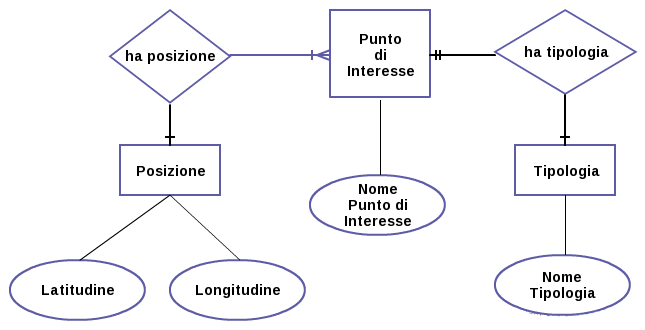
\includegraphics[scale=0.55]{imgs/model/DataModel1.png} 
\caption{Modello dei dati prima iterazione\label{datamodel1iterazione}}
\end{figure}

\paragraph{Diagramma delle classi}

\subsubsection{Modelli comportamentali}
\paragraph{Diagramma di sequenza}
\subsection{Implementazione}
Di seguito sono riportate le porzioni di codice importanti ai fini dell'implementazione del software.
\subsubsection{Connessione al GPS}
\begin{figure}
\begin{center}
\lstset{language=CSharp}
\begin{lstlisting}
async Task<GeoCoordinate> GetPosition()
        {
            if ((bool)IsolatedStorageSettings.ApplicationSettings["LocationConsent"] != true)
            {
                MessageBox.Show("Attivare i servizi di posizionamento");
            }

            Geolocator geolocator = new Geolocator();
            geolocator.DesiredAccuracyInMeters = 50;

            try
            {
                Geoposition geoposition = await geolocator.GetGeopositionAsync(
                    maximumAge: TimeSpan.FromMinutes(5),
                    timeout: TimeSpan.FromSeconds(10)
                    );

                GeoCoordinate coordinateToBack = new GeoCoordinate();
                coordinateToBack.Latitude = geoposition.Coordinate.Latitude;
                coordinateToBack.Longitude = geoposition.Coordinate.Longitude;
                return coordinateToBack;
            }
            catch (ArgumentException AE)
            {
                MessageBox.Show(AE.StackTrace);
            }
        }
\end{lstlisting}
\caption{Prova c\#\label{c}}
\end{center}
\end{figure}


\subsection{Screenshot}





\clearpage

\section{Iterazione 2}

\subsection{Analisi dei requisiti}

\subsubsection{Requisiti funzionali}
Nell'iterazione 2 sono sviluppate le user stories 4,5,6 e 7 (fig. \ref{userstoriestablesecondaiterazione}). 
\begin{figure}
\begin{center}
\begin{tabular}[c]{|c|p{7cm}|c|c|}
\hline
N. & User story & Peso & Priorità\\
\hline
4 & \textit{essendo un utente vorrei poter sapere quando sono vicino ad un punto di interesse per poter conoscere informazioni su di esso} & 5 & 8\\
\hline
5 & \textit{essendo un utente vorrei poter cliccare su un punto di interesse per poter conoscere informazioni su di esso} & 3 & 7\\
\hline
6 & \textit{essendo un utente vorrei poter conoscere i feedback degli altri utenti per poter spostarmi verso punti di interesse dal rating noto} & 3 & 6\\
\hline
7 & \textit{essendo un utente vorrei poter inviare un feedback per condividere la mia esperienza con gli altri utenti} & 5 & 5\\
\hline
\end{tabular}
\caption{Tabella di stima delle user stories della seconda iterazione\label{userstoriestablesecondaiterazione}}
\end{center}
\end{figure}

Considerando queste quattro user stories, possiamo definire i seguenti task che caratterizzano la seconda iterazione:\\
\textbf{Lato client}
\begin{itemize}
\item \textbf{realizzazione form per visualizzazione di informazioni sul punto di interesse};
\item \textbf{realizzazione servizio per la gestione della posizione sulla mappa};
\item \textbf{connessione al servizio di lettura feedback};
\item \textbf{menu contestuale con visualizzazione feedback};
\item \textbf{connessione al servizio di scrittura feedback};
\item \textbf{realizzazione form per inserimento feedback}.
\end{itemize}

\textbf{Lato server}
\begin{itemize}
\item \textbf{creazione servizio per la lettura dei feedback};
\item \textbf{creazione servizio per la scrittura dei feedback}.
\end{itemize}


\subsubsection{Requisiti non funzionali}
Oltre ai requisiti non funzionali già elencati, per l'applicazione si aggiungono i seguenti requisiti:
\begin{itemize}
\item L'applicazione deve gestire la situazione in cui la distanza da due o più punti di interesse sia uguale.
\item L'applicazione deve gestire localmente la vicinanza ai punti di interesse.
\item L'utente può inviare feedback anonimamente.
\item L'utente può inviare al massimo un feedback per ogni punto di interesse.
\item Il commento di feedback deve essere contenuto nei 1000 caratteri.
\end{itemize}

Per il server, invece si può aggiungere:
\begin{itemize}
\item Il sistema deve generare un codice hash per ogni utente.
\end{itemize}



\subsection{Casi di Test}
Dopo l'analisi dei requisiti funzionali e non funzionali, sono stati sviluppati i seguenti casi di test:
\begin{enumerate}
\item Verificare visualizzazione automatica informazioni sul punto di interesse
\begin{enumerate}
\item Assicurarsi che sulla mappa siano visibili i punti di interesse.\\
Assicurarsi della presenza del segnale GPS.\\
Assicurarsi della presenza di una connessione dati attiva.\\
Avvicinarsi fisicamente ad un punto di interesse.\\
\begin{enumerate}
\item Verificare la visualizzazione sul display di informazioni sul punto di interesse.
\item Verificare la possibilità di ritornare alla schermata precedente.
\end{enumerate}
\end{enumerate}
\item Verificare visualizzazione informazioni sul punto di interesse tramite click
\begin{enumerate}
\item Assicurarsi che sulla mappa siano visibili i punti di interesse.\\
Assicurarsi della presenza di una connessione dati attiva.\\
Cliccare sull'icona rappresentante il punto di interesse scelto.
\begin{enumerate}
\item Verificare la visualizzazione di un popup con una voce "visualizza info".
\item Verificare la possibilità di cliccare sulla voce "visualizza info".
\item Verificare la visualizzazione delle informazioni riguardanti il punto di interesse cliccato.
\item Verificare la possibilità di tornare alla schermata precedente.
\end{enumerate}
\end{enumerate}
\item Verificare visualizzazione feedback
\begin{enumerate}
\item Assicurarsi che sulla mappa siano visibili i punti di interesse.\\
Assicurarsi della presenza di una connessione dati attiva.\\
Cliccare sull'icona rappresentante il punto di interesse scelto.
\begin{enumerate}
\item Verificare la visualizzazione di un popup.
\item Verificare la presenza, nella parte superiore del popup, di cinque stelle, colorate a seconda del rating.
\item Verificare la possibilità di tornare alla schermata precedente.
\end{enumerate}
\end{enumerate}
\item Verificare invio feedback
\begin{enumerate}
\item Assicurarsi che sulla mappa siano visibili i punti di interesse.\\
Assicurarsi della presenza di una connessione dati attiva.\\
Cliccare sull'icona rappresentante il punto di interesse scelto.
\begin{enumerate}
\item Verificare la visualizzazione di un popup con una voce "inserisci feedback".
\item Verificare la possibilità di cliccare sulla voce "inserisci feedback".
\item Verificare la visualizzazione sul display di un form perd l'inserimento del feedback.
\item Verificare la possibilità di cliccare sul controllo contenete le cinque stelle.
\item Verificare la possibilità di inserire contenuti nella casella testo.
\item Verificare la possibilità di premere il pulsante "invia" per inviare il feedback.
\end{enumerate}
\end{enumerate}
\end{enumerate}


\subsection{Modellazione}
\subsubsection{Modelli strutturali}
\paragraph{Modello dei dati}
\subparagraph{Client}
Nell'iterazione 1, il client gestisce tre tipologie di dati:
\begin{itemize}
\item \textbf{Punto di interesse}
\item \textbf{Tipologia}
\item \textbf{Posizione}
\end{itemize}
Per cui abbiamo un modello dei dati che può essere sintetizzato come in fig. \ref{datamodel1iterazione}.
\begin{figure}
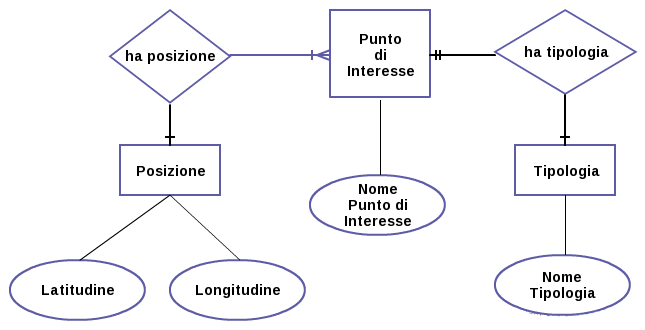
\includegraphics[scale=0.55]{imgs/model/DataModel1.png} 
\caption{Modello dei dati prima iterazione\label{datamodel1iterazione}}
\end{figure}

\paragraph{Diagramma delle classi}

\subsubsection{Modelli comportamentali}
\paragraph{Diagramma di sequenza}
\subsection{Implementazione}

\subsection{Screenshot}


\clearpage

\section{Iterazione 3}

\subsection{Analisi dei requisiti}
\subsubsection{Requisiti funzionali}
Nell'iterazione 3 è sviluppata la user story 8 (fig. \ref{userstoriestableterzaiterazione}). 
\begin{figure}[h!]
\begin{center}
\begin{tabular}[c]{|c|p{6cm}|c|c|}
\hline
N. & User story & Peso & Priorità\\
\hline
8 & \textit{essendo un utente vorrei poter ottenere un itinerario per poter ottimizzare il tempo di visita} & 15 & 5\\
\hline
\end{tabular}
\caption{Tabella di stima delle user stories della terza iterazione\label{userstoriestableterzaiterazione}}
\end{center}
\end{figure}

Considerando tale user story, possiamo definire i seguenti task che caratterizzano la terza iterazione:\\
\textbf{Lato client}
\begin{itemize}
\item \textbf{realizzazione form per visualizzazione dell'itinerario};
\item \textbf{connessione al servizio per la gestione della posizione}.
\end{itemize}

\textbf{Lato server}
\begin{itemize}
\item \textbf{realizzazione servizio per la gestione della posizione};
\item \textbf{realizzazione servizio per la creazione del feedback}.
\end{itemize}

\subsubsection{Requisiti non funzionali}
Oltre ai requisiti non funzionali già descritti nelle precedenti iterazioni, per le funzionalità previste in questa fase, si può aggiungere:
\begin{itemize}
\item L'itinerario deve tener conto della posizione dell'utente ed indicare la direzione
\item L'utente deve poter conoscere in ogni momento la distanza mancante alla fine dell'itinerario.
\end{itemize}

\subsection{Casi di Test}
\subsection{Modellazione}
\subsubsection{Modelli strutturali}
\paragraph{Modello dei dati}
\subparagraph{Client}
Nell'iterazione 1, il client gestisce tre tipologie di dati:
\begin{itemize}
\item \textbf{Punto di interesse}
\item \textbf{Tipologia}
\item \textbf{Posizione}
\end{itemize}
Per cui abbiamo un modello dei dati che può essere sintetizzato come in fig. \ref{datamodel1iterazione}.
\begin{figure}
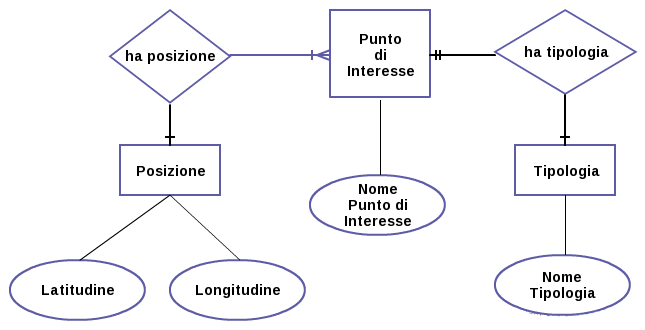
\includegraphics[scale=0.55]{imgs/model/DataModel1.png} 
\caption{Modello dei dati prima iterazione\label{datamodel1iterazione}}
\end{figure}

\paragraph{Diagramma delle classi}

\subsubsection{Modelli comportamentali}
\paragraph{Diagramma di sequenza}
\subsection{Implementazione}
\subsection{Screenshot}

\clearpage
%%%%%%%%%%%%%%%%%%%%%%%%%%%%%%%%%%%%%%%%%%%%%%%%%%%%%%

\clearpage{\pagestyle{empty}\cleardoublepage}
%%%%\clearpage{\pagestyle{empty}\cleardoublepage}
%%%%%%%%%%%%%%%%%%%%%%%%%%%%%%%%%%%%%%%%%%%%%%%%%%%%%%%%%%%
% Capitolo 1

\chapter{Test sul campo}
\label{ref:test}

Introduzione.............

%%%%\clearpage{\pagestyle{empty}\cleardoublepage}
%%%%%%%%%%%%%%%%%%%%%%%%%%%%%%%%%%%%%%%%%%%%%%%%%%%%%%%%%%%
% Capitolo 1

\chapter*{Conclusioni e sviluppi futuri}
\label{ref:conclusioni}  \addcontentsline{toc}{chapter}{Conclusioni e sviluppi futuri}

Introduzione.............

%%%%\clearpage{\pagestyle{empty}\cleardoublepage}

%%%%%%%%%%%%%%%%%%%%%%%%%%%%%%%%%%%%%%%%%%%%%%%%%%%%%%%%%%%%
% Capitolo 1

\chapter{Contesto}
\label{contesto}

In questo capitolo sarà introdotto il distretto Databenc e l'azienda Ancitel. 


\section{DATABENC}
Il progetto Databenc (\url{http://www.databenc.it}) (Distretto Ad Alta Tecnologia per i BENi Culturali) è nato in Campania, grazie all'Università degli Studi di Napoli Federico II e all'Università di Salerno, con l'intento di stabilire una programmazione strategica per valorizzare i beni culturali, il patrimonio ambientale e il turismo.
Databenc ha l'obiettivo di costituire, tra università, centri di ricerca, imprese e amministrazioni comunali presenti sul territorio, una rete che focalizzi le proprie risorse su di un programma di alta tecnologia al fine di creare nuove realtà imprenditoriali (spin-off, start-up), nuove figure professionali, percorsi di alta formazione qualificati, valorizzazione delle conoscenze (brevetti, know how). 
Il distretto è un contenitore in cui riunire ed integrare itinerari eterogenei di ricerca, formazione ed innovazione, con l'obiettivo comune della tutela e della valorizzazione del patrimonio culturale campano inteso in senso esteso: territori, siti, beni e attività. 
\subsection{Le linee di intervento}
Gli ambiti di intervento del Distretto si sviluppano su tre linee portanti: 
\begin{itemize}
\item Conoscenza integrata: la prima forma di tutela di un bene è nella conoscenza e, per tale motivo, è necessario realizzare un esauriente sistema di salvaguardia cognitiva del patrimonio culturale;
\item Monitoraggio diagnostico: ai fini della tutela di un bene risulta indispensabile il monitoraggio diagnostico inteso in senso ampio, che non si limiti solo alla verifica dell'integrità materiale del bene stesso ma si estenda anche all'area in cui il bene è inserito o alle dinamiche turistiche che lo coinvolgono;
\item Fruizione sostenibile: un aspetto fondamentale del bene culturale è quello del suo utilizzo.  Perciò risulta indispensabile conseguire un utilizzo sostenibile del patrimonio culturale.
\end{itemize}

In sintesi, Databenc ha come obiettivo l'introduzione di una nuova ottica con cui affrontare il grave problema della tutela e della valorizzazione del patrimonio culturale, e la creazione di un sistema che faccia della Campania una regione dell'innovazione e un centro di produzione e diffusione di cultura capace di attrarre capitali economici e, soprattutto, capitali umani.


\section{Ancitel}

Ancitel S.p.A. (\url{http://www.ancitel.it}) è la principale società dell'ANCI - Associazione Nazionale Comuni Italiani - e da 25 anni supporta gli enti locali nella gestione di tutti i processi di innovazione.
Dalla sua fondazione, avvenuta nel 1987,  Ancitel affianca le pubbliche amministrazioni locali con un'ampia rete di servizi e progetti ideati per rispondere alle loro esigenze operative quotidiane.
In quanto partner dei Comuni, Ancitel agisce ed opera ogni giorno come centro di competenza per fornire loro soluzioni e strumenti pensati per facilitarne e supportarne l'azione quotidiana ed affrontare le sfide dell'innovazione. 
Grazie ad una profonda conoscenza delle dinamiche interne alla Pubblica Amministrazione, Ancitel ha conseguito notevoli capacità di ascolto, dialogo ed intervento. Per questo uno dei ruoli fondamentali dell'azienda è quello di promuovere e favorire lo scambio delle informazioni tra gli enti pubblici, centrali e locali.
Grazie alle forti competenze e professionalità e alla capacità di valorizzare le esperienze locali e coinvolgere trasversalmente l'intera rete dei Comuni Italiani, Ancitel è stata scelta come partner affidabile dai principali organismi istituzionali italiani, quali Camera dei Deputati, Presidenza del Consiglio dei Ministri, Ministero dell'Ambiente, Ministero dell'Interno, Ministero del Lavoro e delle Politiche Sociali, Ministero dello Sviluppo Economico, Autorità per l'energia elettrica e il gas.
All'interno del distretto Databenc, Ancitel è uno dei principali soci. 


\section{Fruizione informazioni culturali e turistiche in mobilità}
Nell'ambito dei beni culturali, vi sono diversi progetti che coinvolgono enti locali, grandi, piccole e medie imprese ed istituti universitari.
L'obiettivo comune è quello di sviluppare strumenti di valorizzazione e capitalizzazione dell'offerta culturale e delle risorse ambientali, al fine di promuovere e commercializzare l'offerta turistica da parte delle P.A. locali.
Si rende spesso necessaria la definizione e lo sviluppo di una piattaforma abilitante su cui basare servizi per l'offerta culturale. Una piattaforma che ponga al centro le informazioni da offrire agli utenti, che renda facile ed accessibile la fruizione di esse e che possieda validi strumenti per la conservazione e la salvaguardia.
Le stesse informazioni, inoltre, vanno validate e standardizzate, in modo da consentire facilmente l'estrazione e la catalogazione automatica, l'analisi e la correlazione di esse attraverso motori semantici.
%E' altresì auspicabile l'introduzione di un sistema di feedback del bene culturale, in cui è realizzabile il concetto di esplorazione personalizzata in base ad un'analisi delle esperienze degli utenti sul territorio, per comprendere meglio le aspettative del turista influenzato dalle informazioni condivise attraverso i social media.


\clearpage{\pagestyle{empty}\cleardoublepage}


%%%%%%%%%%%%%%%%%%%%%%%%%%%%%%%%%%%%%%%%%%%%%%%%%%%%%%%%%%%%
% Capitolo 2

\chapter{Obiettivi}



\clearpage{\pagestyle{empty}\cleardoublepage}

%%%%%%%%%%%%%%%%%%%%%%%%%%%%%%%%%%%%%%%%%%%%%%%%%%%%%%%%%%%%
% Capitolo 3

\chapter{Ecosistemi mobili}
\label{ecosistemi}
I sistemi operativi per dispositivi mobili sono componenti software che garantiscono il funzionamento di dispositivi quali telefoni cellulari, smartphone, tablet, palmari e lettori MP3, coordinando e gestendo le risorse (hardware e software), e creando un'interfaccia con l'utente.
Diversamente dai sistemi operativi per desktop e laptop, essi devono affrontare problematiche critiche tra cui: limitatezza delle risorse (sia in termini di CPU che di memoria RAM), dimensioni ridotte dello schermo, sistemi touch-screen più o meno avanzati, tecnologie differenti per l'accesso ad Internet, consumo della batteria.
Nell'accezione moderna, il sistema operativo mobile non è solo un prodotto software, ma una vera e propria piattaforma, che mette a disposizione degli sviluppatori delle API su cui sviluppare applicazioni.

Un \emph{ecosistema mobile} è costituito dal sistema operativo, inteso come piattaforma, dagli sviluppatori, che incrementano il numero e migliorano la qualità delle applicazioni disponibili, e dagli utilizzatori, che acquistano sia la piattaforma che le applicazioni nello store.
In questo capitolo verranno trattate i principali sistemi operativi mobile e i relativi frameworks per lo sviluppo delle applicazioni.

\section{Sistemi operativi per dispositivi mobili}

Di seguito una breve descrizione dei sistemi operativi mobili più diffusi.

\subsection{Android}
Android (\emph{\url{http://www.android.com/}}), nato nel 2003, è il più diffuso sistema operativo per dispositivi mobili; open source; distribuito sotto licenza Apache, ovvero vi è la possibilità di modificare e distribuire liberamente il codice sorgente.\\
\begin{figure}
\begin{center}
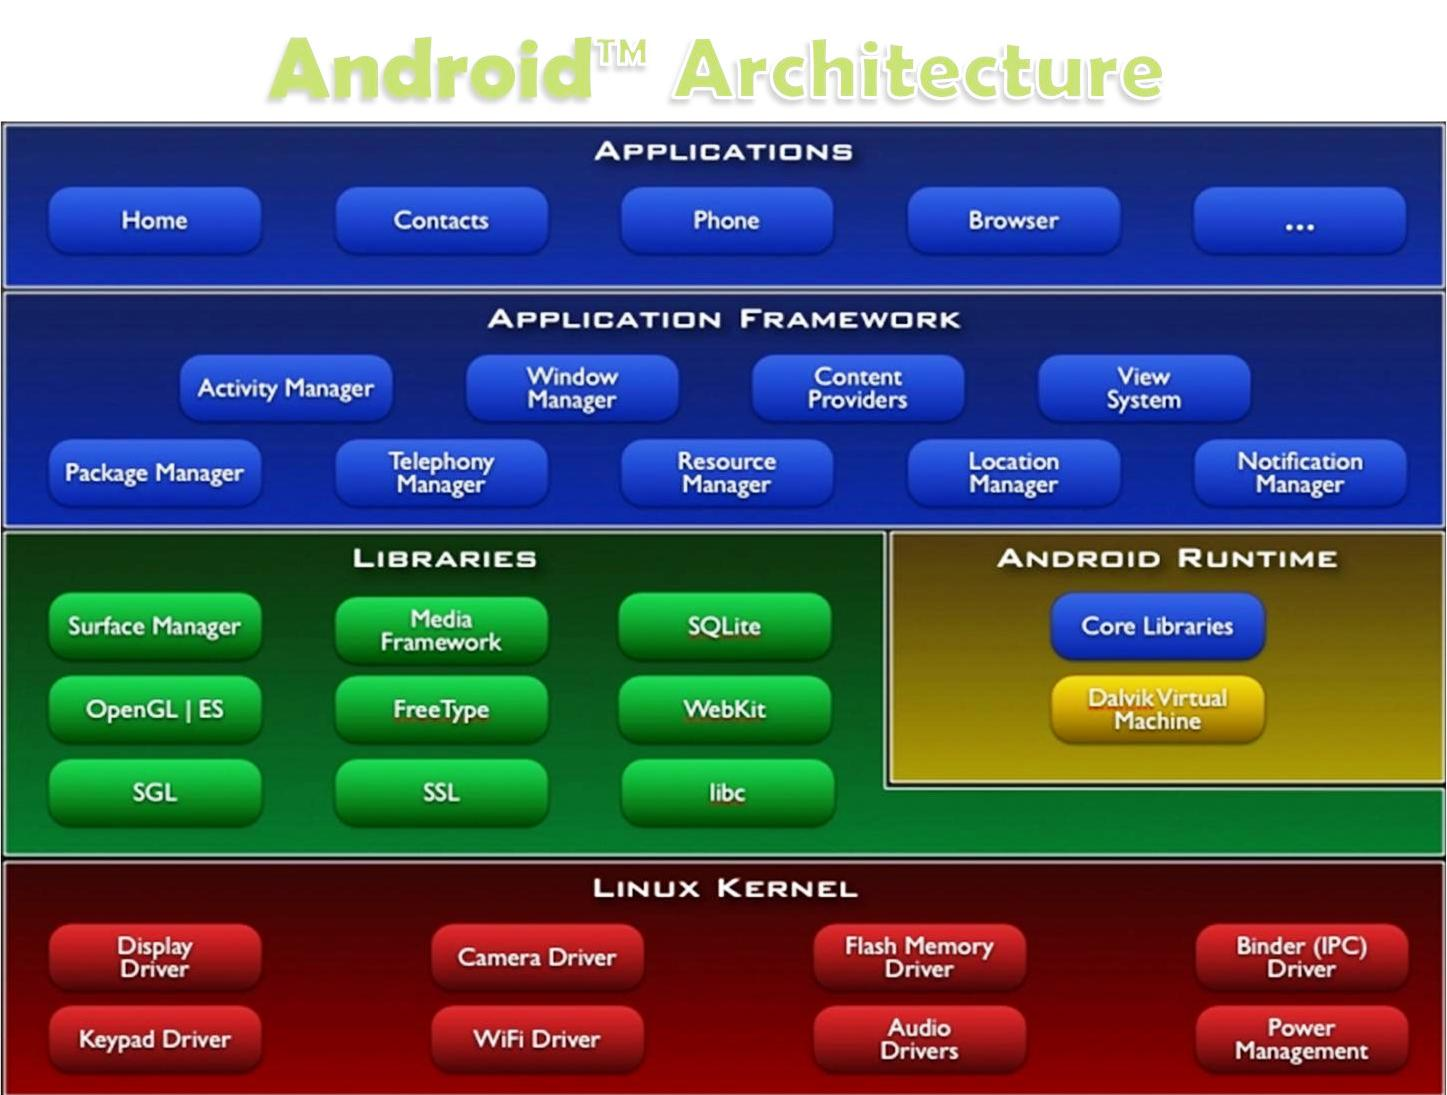
\includegraphics[scale=0.5]{imgs/android_architecture.jpg} 
\caption{Architettura del sistema operativo Android\label{androidarchitecture}}
\end{center}
\end{figure}

L'architettura Android, riportata in figura \ref{androidarchitecture}, è così definita:
\begin{itemize}
\item \emph{kernel}, basato sul kernel Linux(versioni 2.6 e 3.x), contiene i driver per il funzionamento del dispositivo;
\item \emph{strato middleware contenente Librerie ed API}: scritte in C o C++, sono le librerie che forniscono le funzionalità standard al dispositivo, ovvero gestione delle funzioni del display (Surface Manager), gestione dei media (Media Framework), fonts di sistema, DBMS (SQLite), web browser engine (WebKit), e numerose altre;
\item \emph{Android Runtime}: Contiene la Dalvik virtual machine, una macchina virtuale ottimizzata per sfruttare la poca memoria presente nei dispositivi mobili, e che consente di far girare diverse istanze della macchina virtuale contemporaneamente, nascondendo al sistema operativo sottostante la gestione della memoria e dei thread. E' presente, inoltre, un compilatore just-in-time che esegue il Dalvik dex-code, simile al bytecode Java;
\item \emph{Framework di applicazioni che include librerie java basate su Apache Harmony\footnote{Sito internet di riferimento http://harmony.apache.org/}},  costituito da una serie di componenti e API che eseguono numerosi compiti, tra i quali la gestione dell'interazione con l'utente (tramite l'Activity Manager), la condivisione delle informazioni tra i vari processi (Content Provider), gestione delle finestre (Window Manager), gestione delle funzionalità telefoniche (Telephony Manager), ottimizzazione delle risorse (Resource Manager), gestione del ciclo di vita delle applicazioni (Package Manager), gestione della localizzazione (Location Manager), gestione delle notifiche con l'utente (Notification Manager).
\end{itemize}

Per quanto riguarda gli aggiornamenti, Android ha un rapido ciclo di rilascio (nuove versioni ogni sei-nove mesi).
Gli aggiornamenti sono in genere di natura incrementale e apportano miglioramenti del software a intervalli regolari. Tra una major release e l'altra vengono messi a disposizione rilasci intermedi per risolvere problemi di sicurezza e altri bug del software.
\\


\subsubsection{Sviluppo Applicazioni}
Tutte le applicazioni Android, dovendo basarsi sul framework di librerie Java, sono scritte in Java.

L'Android software development kit SDK (\emph{\url{http://developer.android.com/sdk/}}) include un insieme di tool di sviluppo, quali un debugger, librerie, un emulatore basato su QEMU (\emph{\url{http://wiki.qemu.org/}}), codici di esempio e tutorials.
Le piattaforme di sviluppo supportate includono computer con sistema operativo Linux, MAC OS X (dalla 10.5.8) e Windows (da XP).
L'IDE (Integrated Development Enviroment) ufficialmente supportato è ADT (Android Development Tools), basato su Eclipse (\emph{\url{http://www.eclipse.org/}}) ma, in ogni caso, è possibile sviluppare applicazioni Android anche con altri IDE.

\subsection{iOS}
iOS (\emph{\url{http://www.apple.com/it/ios/}}) è un sistema operativo di Apple, derivato da Unix BSD ed ha un microkernel XNU Mach basato su Darwin OS.
Nato nel 2007, è rilasciato sotto licenza APSL (Apple Public Source License), che consente agli utenti di migliorare il software ma non di rilasciarlo.\\

\begin{figure}[h!]
\begin{center}
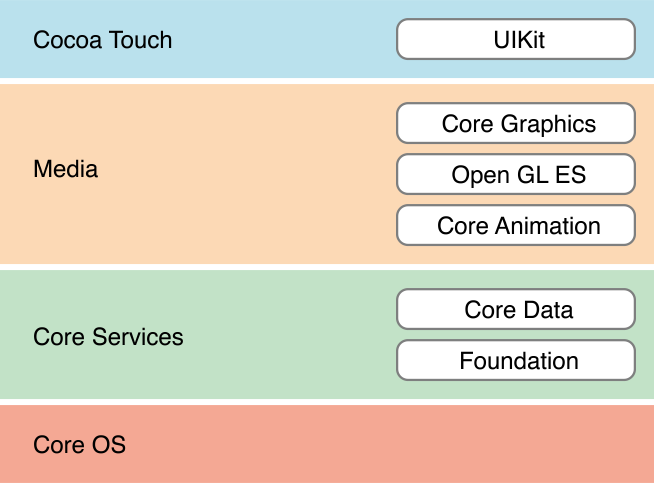
\includegraphics[scale=0.5]{imgs/ios_architecture.png} 
\caption{Architettura del sistema operativo iOS\label{iosarchitecture}}
\end{center}
\end{figure}

iOS ha quattro livelli di astrazione, riportati in figura \ref{iosarchitecture}:
\begin{itemize}
\item \emph{Core OS Layer}: contiene le caratteristiche di basso livello su cui sono basate la maggior parte delle tecnologie. Contiene il kernel ed interfacce di basso livello UNIX. Gestisce la memoria virtuale, i threads, il filesystem e i driver delle periferiche.
Sono presenti, inoltre, framework per l'esecuzione di DSP, calcoli di algebra lineare ed elaborazione delle immagini ; framework per la gestione del Bluetooth; framework per la gestione degli accessori hardware eventualmente connessi al dispositivo; framework per la sicurezza;
\item \emph{Core Services Layer}: contiene i servizi di sistema fondamentali che tutte le applicazioni usano. Offre quindi servizi di alto livello basati sui Core Service Frameworks, ad esempio lo storage di dati in remoto (iCloud); la protezione dei dati sensibili, per evitare che applicazioni malevole facciano uso di essi; la gestione dei documenti XML; la possibilità di condividere dati tra le varie applicazioni;
\item \emph{Media Layer}: contiene le tecnologie grafiche, audio e video;
\item \emph{Cocoa Touch Layer}: contiene i framework indispensabili per costruire applicazioni iOS (Cocoa Service Framework) e definisce l'infrastruttura di base ed il supporto per tecnologie fondamentali come il multitasking, l'input basato sul touch, le notifiche in push e locali e molti altri servizi di alto livello.
\end{itemize}

Apple rilascia aggiornamenti di iOS circa una volta l'anno. Tali aggiornamenti costituiscono revisioni complete del sistema operativo.
\subsubsection{Sviluppo Applicazioni}
Le applicazioni per iOS possono essere sviluppate tramite l'iOS SDK (\emph{\url{http://developer.apple.com/}}),  disponibile solo su sistema operativo MAC OS X. Esse sono scritte in Objective-C, anche se esiste il supporto per C e C++.

L'IDE di riferimento per lo sviluppo di applicazioni per iOS è XCode, che include un editor di sorgenti; uno strumento per disegnare le interfacce utente; il compilatore LLVM  e un emulatore, oltre ad altri numerosi tool per il debug, il testing e la gestione degli errori.


\subsection{Windows Phone OS}
Windows Phone OS (\emph{\url{http://www.windowsphone.com/it-it}}) è un sistema operativo Microsoft, nato nel 2010, orientato ai dispositivi mobile. E' il successore di Windows Mobile, sistema operativo nato nel 1996 per i palmari, ma è completamente differente da quest'ultimo.

E' distribuito con licenza Microsoft EULA, per cui è soggetto a limitazioni d'uso, di garanzia e di responsabilità.

\begin{figure}
\begin{center}
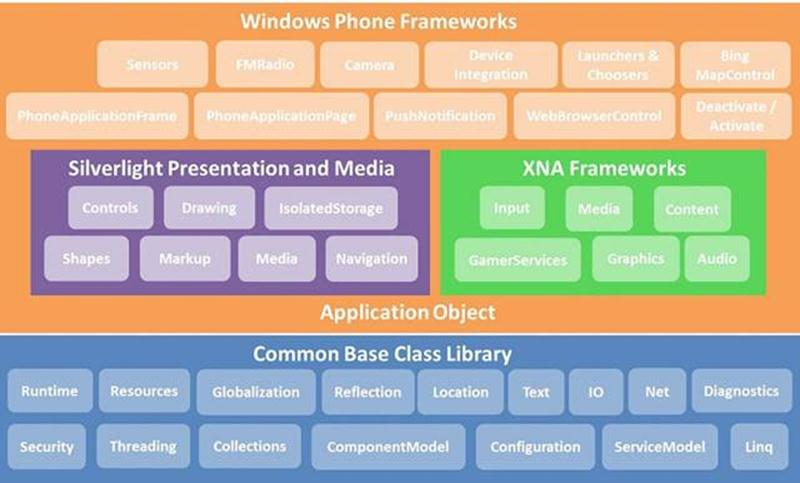
\includegraphics[scale=0.7]{imgs/windowsphone_architecture.jpg} 
\caption{Architettura del sistema operativo iOS\label{wparchitecture}}
\end{center}
\end{figure}

Windows Phone OS ha un'architettura a quattro livelli, come rappresentato in figura \ref{wparchitecture}:
\begin{itemize}
\item \emph{Common Base Class Library}: è una libreria standard che include un vasto numero di funzionalità comuni, come ad esempio la lettura e scrittura su un file, il rendering grafico, l'interazione con i database, la manipolazione di documenti XML e il supporto per il multithreading;
\item \emph{Silverlight Presentation and Media}: fornisce librerie per la navigazione, la grafica, la gestione dei media;
\item \emph{XNA Frameworks}: è un insieme di librerie, servizi e risorse per la gestione dell'accelerazione grafica e del rendering, dell'audio e dei servizi di autenticazione e connettività;
\item \emph{Windows Phone Frameworks}: definisce dei blocchi comuni per tutte le applicazioni Windows Phone. Esso fornisce l'interfaccia al sistema ed alle risorse hardware, ovvero i sensori, l'accelerometro, il compasso, il giroscopio e la fotocamera. In Windows Phone Framework è presente anche un sistema di notifiche.
\end{itemize}

\subsubsection{Sviluppo Applicazioni}
Le applicazioni per Windows Phone possono essere scritte in C++, C\#, C, Visual Basic e HTML5, grazie al vasto supporto del framework .NET.
La più recente versione della Windows Phone SDK (\emph{\url{http://dev.windowsphone.com/}}) è disponibile solo per sistemi operativi Windows 8 a 64bit.

L'IDE di riferimento per lo sviluppo di applicazioni Windows Phone è Visual Studio per Windows Phone, che include un editor di sorgenti, di testing, di debug, di gestione delle risorse e del ciclo di vita dell'applicazione.
Microsoft mette inoltre a disposizione altri significativi tools come Express Blend, che permette di creare interfacce utente; Silverlight (\emph{\url{http://www.microsoft.com/silverlight/}}) e XNA per la gestione della grafica 2D e 3D; Windows Phone Emulator, l'emulatore dei dispositivi Windows Phone.\\


\clearpage{\pagestyle{empty}\cleardoublepage}

%%%%%%%%%%%%%%%%%%%%%%%%%%%%%%%%%%%%%%%%%%%%%%%%%%%%%%%%%%%%
% Capitolo 4

\chapter{Tecnologie}
\label{tecnologie}





In questo capitolo verranno introdotte le principali tecnologie di 
localizzazione, di mapping e le architetture.

 RISCRIVERE!!!!


\section{Serializzazione}
La serializzazione è un processo  per salvare un oggetto in un supporto di memorizzazione lineare o per trasmetterlo su una connessione di rete.
Essa può essere realizzata in modalità binaria o testuale.
La modalità binaria, seppur molto efficiente, presenta scarsa interoperabilità e flessibilità.
La serializzazione testuale, invece, essendo basata sulla tecnologia REST, determina un'ottimizzazione nello scambio di informazioni tra ambienti eterogenei, rendendo le strutture tradotte indipendenti dall'architettura e dalle differenti rappresentazioni dei dati.
I formati di serializzazione testuale più noti sono XML, JSON e YAML, che  sono trattati di seguito.

\subsection{XML}
La storia di XML (eXtra Markup Language)\footnote{Il formato XML è uno standard gestito dalla W3C. Il sito internet di riferimento è \emph{\url{http://www.w3.org/XML/}}} è strettamente legata a quella di SGML (Standard Generalized Markup Language), progetto ideato da IBM per migliorare l'interoperabilità aziendale, dal momento che la comunicazione tra computer era ostacolata da una ricca gamma di formati di file.

XML, infatti, è nato grazie ad una semplificazione di SGML per consentire di definire in maniera semplice nuovi linguaggi di markup da utilizzare in ambito web.
In definitiva, XML è un linguaggio marcatore basato su un meccanismo sintattico che consente di definire e controllare il significato degli elementi contenuti in un documento o in un testo.

\begin{figure}
\begin{center}
\lstset{language=MYXML}
\begin{lstlisting}
<?xml version="1.0" encoding="utf-8"?>
<!DOCTYPE Rubrica SYSTEM “Rubrica.dtd”>
<rubrica>
	<persona>
		<nome>Enrico</nome>
		<cognome>Bencivenga</cognome>
		<indirizzo>
			<via>Camillo Cucca 106</via>
			<cap>80031</cap>
			<citta>Brusciano</citta>
			<provincia>Napoli</provincia>
		</indirizzo>
	</persona>
</rubrica>

\end{lstlisting}
\caption{Esempio di documento XML\label{xmlimage}}
\end{center}
\end{figure}


\subsubsection{Sintassi}
XML è una tecnologia adoperata per creare linguaggi di markup che descrivono dati di qualsiasi tipo, quindi consente di descrivere dati in modo accurato creando nuovi tag.
Un esempio di sintassi XML è l'esempio \textbf{Rubrica.xml} della figura \ref{xmlimage}.


Un documento XML si può quindi dividere in due sezioni: il \textit{prologo} e l'\textit{istanza}. 
Il prologo contiene informazioni di carattere generale sul documento, mentre l'istanza contiene i dati. Il documento XML è costituito da un insieme di dati e di marcatori che ne specificano la struttura.
Alcuni di essi sono:
\begin{itemize}
\item Tag;
\item Processing instructions;
\item Entità;
\item Commenti;
\item Sezione CDATA.
\end{itemize}

\paragraph{Dichiarazione}
Le prime due righe contenute nell'esempio della figura \ref{xmlimage} costituiscono la dichiarazione del documento XML.
La prima riga contiene la specifica della versione di XML utilizzata e del tipo di codifica del documento. 
Nella seconda riga è stabilita la tipologia di documento alla quale appartiene il file, specificando il particolare schema DTD scelto.
La dichiarazione della tipologia di documento può essere di tre tipi:
\begin{itemize}
\item \textbf{Esterna}:
\lstset{language=MYXML}
\begin{lstlisting}
<!DOCTYPE ELEMENTO_ROOT SYSTEM "nomefile.dtd”>
\end{lstlisting}
\item \textbf{Interna}:
\begin{lstlisting}
<!DOCTYPE ELEMENTO_ROOT [CONTENUTO DTD SCHEMA]>
\end{lstlisting}
\item \textbf{Mista}:
\begin{lstlisting}
<!DOCTYPE ELEMENTO_ROOT SYSTEM "nomefile.dtd”
[CONTENUTO DTD SCHEMA]>
\end{lstlisting}
\end{itemize}

\paragraph{Tag}
L'elemento radice della figura \ref{xmlimage} è il tag \textbf{<rubrica>}, che contiene all'interno tutti gli altri elementi del documento.
Inserire più di un elemento radice è considerato errato. I tag interni sono definiti elementi \textit{child}, e sono parte dell'organizzazione gerarchica di XML.
I tag di apertura e di chiusura vanno sempre specificati, tranne nel caso non vi siano informazioni in essi. Per gli elementi vuoti XML prevede una sintassi abbreviata \textbf{<tag/>}.

\paragraph{Attributi}
I tag XML possono contenere informazioni interne che vengono definite \textit{attributi} del tag. Essi specificano proprietà intrinseche al tag e vanno indicati attraverso l'accoppiata nome-valore, come ad esempio:
\lstset{language=MYXML}
\begin{lstlisting}
<Telefono tipo="cellulare">3289196064</Telefono>
\end{lstlisting}.


\paragraph{Commenti}
Oltre alle direttive di elaborazione, in un file XML è possibile individuare i commenti, racchiusi tra le sequenze di caratteri \textbf{<!--} e \textbf{-->}. Questi possono trovarsi in qualsiasi punto del documento, ed il testo contenuto non viene elaborato dal parser.


\begin{figure}[h]
\lstset{language=MYXML}
\begin{lstlisting}
<! ELEMENT persona (nome, cognome)>
<! ELEMENT nome (#PCDATA) >
<! ELEMENT cognome (#PCDATA) >
\end{lstlisting}
\caption{Esempio di file DTD\label{dtdimage}}
\end{figure}

\paragraph{Correttezza sintattica e validità}
Un documento XML è valido se è conforme al DTD associato.
Un DTD (Document Type Definition) è uno strumento che definisce le componenti ammesse nella costruzione di un XML. Un esempio di DTD è riportato in figura \ref{dtdimage}.





Un documento XML, in ogni caso, non deve essere necessariamente valido, ma il requisito essenziale è la correttezza nella sintassi.
Tali regole sintattiche possono essere riassunte in:
\begin{itemize}
\item Deve essere presente un solo elemento radice;
\item I tag non possono iniziare con numeri o caratteri speciali e contenere spazi;
\item I tag devono essere innestati correttamente;
\item Tutti i tag e gli attributi sono espressi in minuscolo;
\item E' obbligatorio inserire i tag di chiusura, sia in forma estesa che in forma abbreviata, ove consentito.
\end{itemize}
Se un documento è sintatticamente valido, può essere analizzato da un \textit{parser}, un programma che, analizzando la struttura grammaticale del documento XML, ne ricostruisce l'albero a partire dall'elemento radice e proseguendo con gli elementi child.


\subsection{JSON}
JSON (JavaScript Object Notation) è un formato di serializzazione nato appositamente per lo scambio dei dati.
Un documento JSON è di facile interpretazione anche senza il processo di parsing, data la leggibilità della sua struttura.

JSON è completamente indipendente dal linguaggio di programmazione utilizzato, in quanto utilizza convenzioni conosciute dai programmatori di linguaggi della famiglia del C. 
Grazie a queste caratteristiche, JSON è un linguaggio ideale per lo scambio dei dati e per l'interoperabilità.
Con JSON è possibile rappresentare quattro tipi primitivi:
\begin{itemize}
\item numeri;
\item stringhe;
\item variabili booleane;
\item NULL.
\end{itemize}
e due tipi strutturati:
\begin{itemize}
\item array;
\item oggetti.
\end{itemize}

Il formato JSON è ampiamente diffuso, soprattutto tra gli sviluppatori web, per le dimensioni inferiori dello stream dati, dovute alla sua bassa ridondanza.

\subsubsection{Sintassi}
La sintassi JSON è molto semplice e si basa su due strutture:
\begin{itemize}
\item \textbf{coppia nome/valore}, realizzabile in diversi linguaggi di programmazione come un oggetto, un record, uno struct, una tabella hash, un elenco di chiavi o un array associativo;
\item \textbf{elenco ordinato di valori}, realizzabile nella maggior parte dei linguaggi di programmazione con un array, un vettore, un elenco o una sequenza.
\end{itemize}
Queste due strutture sono utilizzabili in tutti i linguaggi di programmazione, e ciò rende ancora più evidente la natura di JSON, orientata all'interoperabilità.

\begin{figure}
\lstset{language=JSON}
\begin{lstlisting}
{"nome": "enrico"}
\end{lstlisting}
\caption{Esempio di oggetto JSON\label{jsonobjectimage}}
\end{figure}
\paragraph{Oggetto}
Un oggetto in JSON è contenuto tra due parentesi graffe. Tra il nome e il valore sono presenti due punti ed il nome dell'oggetto è scritto tra due doppi apici, mentre il valore è scritto tra due doppi apici nel caso non sia numerico. Un esempio è in figura\ref{jsonobjectimage}.

\begin{figure}
\lstset{language=JSON}
\begin{lstlisting}
{"serializzazione": ["XML", "JSON", "altro"]}
\end{lstlisting}
\caption{Esempio di oggetto JSON\label{jsonarrayimage}}
\end{figure}

\paragraph{Array}
Un array è una raccolta ordinata di valori. In JSON un array è contenuto tra due parentesi quadre e i valori sono separati da virgola, come è evidente dalla figura \ref{jsonarrayimage}.

Le stringhe sono rappresentate come nella maggior parte dei linguaggi di programmazione e vanno sempre messe tra doppi apici, mentre i numeri possono iniziare con identificatori di segno ed essere seguiti da una parte esponenziale, così come in molti linguaggi.
Solo le rappresentazioni esadecimali o ottali non sono permesse.
\begin{figure}
\lstset{language=JSON}
\begin{lstlisting}
{
  "rubrica": {
    "persona": {
      "nome": "Enrico",
      "cognome": "Bencivenga",
      "indirizzo": {
        "via": "Camillo Cucca 106",
        "cap": "80031",
        "citta": "Brusciano",
        "provincia": "Napoli"
      }
    }
  }
}
\end{lstlisting}
\caption{Esempio di oggetto JSON\label{jsonimage}}
\end{figure}

Nell'immagine \ref{jsonimage} è possibile visualizzare un esempio completo di file JSON, analogo a quello precedente di file XML in figura \ref{xmlimage}.
L'indentazione è utilizzata solo a scopo di chiarezza sintattica, ma il testo si estende su di una sola riga, senza caratteri di ritorno a capo.
Naturalmente anche un documento JSON può essere elaborato da un parser e ricostruito.

\subsection{YAML}
YAML (YAML Ain't Markup Language), sito web di riferimento \emph{\url{http://yaml.org}}, è un linguaggio nato nel 2001 con l'obiettivo di essere \textit{human-friendly}.
E' progettato per persone che lavorano con dati, grazie alla sua comprensibilità ed interoperabilità.
YAML è peraltro un linguaggio molto pulito, in quanto riduce al minimo la quantità di caratteri strutturali e permette di mostrare i dati in modo naturale e significativo.
Gli obiettivi di YAML sono:
\begin{itemize}
\item semplicità di lettura;
\item corrispondenza con i tipi per la maggioranza dei linguaggi di programmazione;
\item esportabilità dei dati;
\item estendibilità;
\item facilità di implementazione e usabilità.
\end{itemize}

\subsubsection{Sintassi}
YAML mette a disposizione due tipi di sintassi, una indentata e una in linea, simile al formato JSON.
Inoltre in YAML ci sono degli indicatori che servono a descrivere la struttura ed il contenuto di un documento YAML.

\begin{figure}
\lstset{language=YAML}
\begin{lstlisting}
--- # Discipline
 - Matematica
 - Informatica
 - Fisica
\end{lstlisting}
\caption{Lista nel formato indentato YAML\label{yamllistaimage}}
\end{figure}

\begin{figure}
\lstset{language=YAML}
\begin{lstlisting}
 --- # Discipline
 [Matematica, Informatica, Fisica]
\end{lstlisting}
\caption{Lista nel formato convenzionale YAML\label{yamllistbimage}}
\end{figure}

\begin{figure}
\lstset{language=YAML}
\begin{lstlisting}
--- # Blocco indentato
   nome: Enrico Bencivenga
   eta: 30
 --- # Blocco allineato
 {nome: Enrico Bencivenga, eta: 30}
\end{lstlisting}
\caption{Array in YAML\label{yamlarrayimage}}
\end{figure}

\begin{figure}
\lstset{language=YAML}
\begin{lstlisting}
 --- |
	Questa è la 
		tesi di laurea
			in Ingegneria Informatica
		di Enrico Bencivenga
	matr. 534000442
\end{lstlisting}
\caption{Stringa nel formato indentato YAML\label{yamlstringaimage}}
\end{figure}

\begin{figure}
\lstset{language=YAML}
\begin{lstlisting}
 --- >
Questa è la 
tesi di laurea
in Ingegneria Informatica
di Enrico Bencivenga
matr. 534000442
\end{lstlisting}
\caption{Stringa nel formato convenzionale YAML\label{yamlstringbimage}}
\end{figure}

\paragraph{Liste}
Le liste sono collezioni di elementi. La loro rappresentazione in YAML può essere indentata (fig. \ref{yamllistaimage}) o allineata (fig. \ref{yamllistbimage}).

\paragraph{Array associativi}
Gli array sono associazioni nome/valore, e possono essere rappresentati come in figura \ref{yamlarrayimage}.

\paragraph{Stringhe}
Le stringhe non richiedono gli apici o i doppi apici per essere rappresentate.

La rappresentazione delle stringhe può essere indentata, come nella figura \ref{yamlstringaimage}, oppure allineata, come nella figura \ref{yamlstringbimage}, dove il testo viene allineato in un singolo paragrafo.

\subsubsection{Confronto tra XML, JSON e YAML}
JSON è caratterizzato dalla semplicità di rappresentazione delle strutture dati e da una bassa ridondanza, dovuta all'assenza dei tag di chiusura; è molto facile da interpretare e per questo si adatta alle applicazioni web-based.\\

YAML ha caratteristiche aggiuntive rispetto a JSON, quali l'estensibilità dei tipi, la rappresentazione di stringhe senza apici, gli anchors e gli aliases. Anche YAML risulta molto adatto alle applicazioni web-based.\\
XML ha più vincoli di YAML e JSON, poichè è nato per essere compatibile con SGML, ma risulta più adatto alla descrizione di strutture dati e presenta uno spettro di utilizzo più vasto.

\section{Web Service}
Un \textit{Web Service} è, secondo la definizione data dal \textit{W3C}, un sistema software progettato per supportare l'interoperabilità tra diversi elaboratori su di una medesima rete ovvero in un contesto distribuito. L'interoperabilità è ottenuta associando all'applicazione un'interfaccia software (descritta in formato automaticamente elaborabile, ad esempio il Web Services Description Language), che espone all'esterno i servizi associati e utilizzando la quale altri sistemi possono interagire con l'applicazione stessa, attivando le operazioni descritte nell'interfaccia tramite appositi messaggi di richiesta.
Tali messaggi sono formattati secondo gli standard XML ed incapsulati e trasportati tramite i protocolli web (di solito HTTP), da cui il nome web service. Un esempio di trasporto è in figura \ref{webservice}.
\begin{figure}
\begin{center}
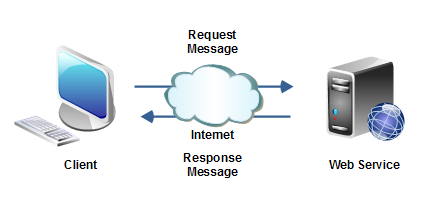
\includegraphics[scale=1]{imgs/webservice.png} 
\caption{Scambio messaggi in un Web Service\label{webservice}}
\end{center}
\end{figure}
I \textit{Web Service} hanno ridefinito nel tempo il modo in cui viene utilizzato il Web, che è visto non più come strumento di pubblicazione e consultazione di pagine statiche, ma anche e soprattutto come strumento per elaborare dati, interagire, integrare le applicazioni e creare business.
Questa nuova generazione di applicazioni internet consente ai privati di accedere a servizi studiati appositamente per le loro esigenze, ed alle aziende di comunicare e gestire i rapporti con clienti, partner e fornitori in modo semplice e immediato.
L'accesso ai Web Service è possibile da qualunque dispositivo in grado di interagire con la rete, ovvero PC, smartphone, palmari o notebook.\\
Un Web Service può essere scritto in qualsiasi linguaggio di programmazione e, come tutte le applicazioni web, ha la caratteristica fondamentale di trasmettere informazioni in formato testuale attraverso protocolli di tipo request-reply (HTTP).
Solitamente, un Web Service comunica con i browser tramite pagine HTML, incapsulate all'interno di una risposta HTTP; diversamente, nella comunicazione tra Web Service o tra Web Service e applicazioni le informazioni sono scambiate in maniera strutturata (cioè capaci di autodescriversi in modo da essere comprensibili sia ad un agente software che ad un umano).
I formati di descrizione sono naturalmente i formati di serializzazione dei dati trattati precedentemente, ovvero XML, JSON e YAML, la cui caratteristica principale è quella di essere testi semplici da cui estrarre informazioni tramite il parsing.\\
I protocolli per i web service utilizzano tre architetture diverse:
\begin{itemize}
\item \textbf{RPC oriented};
\item \textbf{Message oriented};
\item \textbf{REST}.
\end{itemize}
\subsection{RPC oriented}
L'architettura RPC oriented è basata sul concetto ri Remote Procedure Call dei middleware tradizionali.
Quindi, il client invia al server una richiesta, contenente il nome della procedura remota da invocare e i parametri, usando l'operazione POST del protocollo HTTP; Il server invia il risultato al client come risposta HTTP.
\subsubsection{XML-RPC}
Il primo protocollo specificamente sviluppato per i Web Service è stato \textit{XML-RPC}, in cui la richiesta e la risposta del messaggio sono formulate in linguaggio XML.
XML-RPC sfrutta la disponibilità di parser XML su tutte le principali piattaforme e la facilità con cui si possono generare documenti XML.
Le principali carenze di XML-RPC sono l'assenza di meccanismi per la gestione di tipi di dato non supportati; il mancato supporto nativo di funzionalità avanzate come autenticazione e gestione delle transazioni; mancanza di definizione formale delle interfacce delle procedure remote, per cui eventuali errori o incongruenze sono scoperti solo a tempo di esecuzione.
Per ovviare a tali limiti è stato introdotto \textbf{SOAP}
\subsubsection{SOAP}
Acronimo di \textit{Simple Object Access Protocol}, SOAP (\emph{\url{www.w3.org/TR/soap/}}) è basato su XML ed è accattato come standard dal consorzio W3C.
SOAP è supportato dai principali ambienti di sviluppo e ha la caratteristica di separare il formato dei messaggi dal modo in cui sono veicolati attraverso un protocollo già esistente. 
SOAP può utilizzare protocolli diversi da HTTP, come SMTP.
I vantaggi dell'utilizzo di SOAP, rispetto ad XML-RPC sono prevalentemente nella versatilità, dal momento che SOAP consente di estendere l'insieme dei tipi da usare come parametri e valori di ritorno e consente di estendere il protocollo stesso al fine di aggiungere funzionalità come la sicurezza o la gestione delle transizioni senza perdere l'interoperabilità.
Per la definizione formale dell'interfaccia, SOAP ricorre a \textbf{WSDL}.
\subsubsection{WSDL}
WSDL, ovvero \textit{Web Service Description Language} è un linguaggio per definire le interfacce dei Web Service basati su SOAP.
Anch'esso è uno standard W3C ed è naturalmente basato su XML.
Un documento WSDL contiene una specifica "machine-readable" di:
\begin{itemize}
\item punti di accesso ai web service
\item protocolli utilizzati
\item operazioni disponibili, con i rispettivi parametri di ritorno
\item tipi non predefiniti usati dalle operazioni
\end{itemize}
Anche se in teoria un documento WSDL dovrebbe essere in un formato leggibile e modificabile da un essere umano, in pratica il formato è piuttosto complesso e si rende necessaria la generazione del documento tramite appositi tool e librerie, offerti dai principali ambienti di sviluppo.
Tipicamente il WSDL è disponibile online sul sito che ospita il web service ed è utilizzato a tempo di esecuzione sia per verificare che non ci siano modifiche dell'interfaccia server, sia per creare le classi che rappresentano la comunicazione col client.
Un esempio di WSDL è riportato in figura \ref{wsdlimage}.
\begin{figure}[h!]
\begin{center}
\lstset{language=MYXML}
\begin{lstlisting}
<?xml version="1.0"?> 
<wsdl:description xmlns:wsdl="http://www.w3.org/ns/wsdl"
  xmlns:wsoap= "http://www.w3.org/ns/wsdl/soap"
  xmlns:hy="http://www.herongyang.com/Service/"
  targetNamespace="http://www.herongyang.com/Service/">

  <wsdl:documentation>
    Hello_WSDL_20_SOAP.wsdl
    Copyright (c) 2009 by Dr. Herong Yang, herongyang.com
    All rights reserved
  </wsdl:documentation>

  <wsdl:types>
    <xsd:schema xmlns:xsd="http://www.w3.org/2001/XMLSchema"
      targetNamespace="http://www.herongyang.com/Service/">
      <xsd:element name="Hello" type="xsd:string"/>    
      <xsd:element name="HelloResponse" type="xsd:string"/>    
    </xsd:schema>    
  </wsdl:types>

  <wsdl:interface name="helloInterface" >
    <wsdl:operation name="Hello" 
      pattern="http://www.w3.org/ns/wsdl/in-out" 
      style="http://www.w3.org/ns/wsdl/style/iri">
      <wsdl:input messageLabel="In" 
        element="hy:Hello" />
      <wsdl:output messageLabel="Out" 
        element="hy:HelloResponse" />
    </wsdl:operation>
  </wsdl:interface>

  <wsdl:binding name="helloBinding" 
    interface="hy:helloInterface"
    type="http://www.w3.org/ns/wsdl/soap"
    wsoap:protocol="http://www.w3.org/2003/05/soap/bindings/HTTP/">
    <wsdl:operation ref="hy:Hello" 
      wsoap:mep="http://www.w3.org/2003/05/soap/mep/soap-response"/>
  </wsdl:binding>

  <wsdl:service name="helloService" 
    interface="hy:helloInterface">
    <wsdl:endpoint name="helloEndpoint" 
      binding="hy:helloBinding"
address="http://www.herongyang.com/Service/Hello_SOAP_12.php"/>
  </wsdl:service>

</wsdl:description>
\end{lstlisting}
\caption{Esempio di documento WSDL\label{wsdlimage}}
\end{center}
\end{figure}
La combinazione SOAP+WSDL consente di realizzare web service con uno sforzo di programmazione contenuto, sia lato client che lato server e, grazie all'uso del servizio \textbf{UDDI}, garantisce ed aumenta l'interoperabilità.
\subsubsection{UDDI}
UDDI (\textit{Universal Description Discovery and Integration}) è un web service basato su SOAP+WSDL che realizza un repository di descrizioni WSDL con funzioni di pubblicazione e ricerca di web service in base ad una serie di metadati.
Lo standard UDDI originariamente ipotizzava lo sviluppo di un \textit{Universal Business Registry} pubblivo che consentisse una ricerca globale dei web service, ma attualmente l'idea dell'UBR è stata abbandonata ed il servizio UDDI è utilizzato soprattutto in abito intranet come repository centralizzato di documenti WSDL.
\subsection{Message oriented}
In un'architettura di servizi Message oriented le diverse applicazioni si scambiano messaggi unidirezionali che hanno le seguenti caratteristiche:
\begin{itemize}
\item il focus è sul messaggio più che sull'operazione;
\item se una richiesta genera una risposta, questa è inviata con un messaggio indipendente dal messaggio di richiesta;
\item il servizio non è tenuto a elaborare i messaggi che riceve in ordine di ricezione;
\item è sfumata la distinzione tra client e server: l'architettura è peer-to-peer.
\end{itemize}

I vantaggi dell'utilizzo di un'architettura Message oriented sono il disaccoppiamento anche temporale tra client e server, infatti, se il server non è momentaneamente disponibile, il messaggio può essere mantenuto in una coda; la maggiore flessibilità nella distribuzione (smistamento intelligente dei messaggi tra più server); flessibilità nell'ordine delle operazioni (priorità diverse per i messaggi).

\subsection{REST}
Representational state transfer (REST)\footnote{Il paradigma REST è stato introdotto nel 2000 nella tesi di dottorato di Roy Fielding, reperibile all'indirizzo \emph{\url{http://www.ics.uci.edu/~fielding/pubs/dissertation/rest_arch_style.htm}}} è un tipo di architettura software per i sistemi di ipertesto distribuiti come il World Wide Web.
Esso si riferisce ad un insieme di principi di architetture di rete, i quali delineano come le risorse sono definite e indirizzate. Il termine è spesso usato nel senso di descrivere ogni semplice interfaccia che trasmette dati su HTTP senza un livello opzionale come SOAP o la gestione della sessione tramite i cookie.

Le applicazioni basate sui principi REST, spesso definite "RESTful", usano richieste HTTP per inviare dati (creare o aggiornare), leggere dati (eseguire query) e cancellare dati.

Nel dettaglio, lo stile architetturale di REST, rappresentato in figura \ref{restimage}, consiste di un lato client e un lato server: i client inviano richieste ai server; i server elaborano tali richieste e restituiscono ai client i risultati delle elaborazioni.
Richieste e risposte si basano sul trasferimento di rappresentazioni di \textbf{risorse}.

L'esistenza delle risorse è un concetto importante in REST, in quanto esse sono fonti di informazioni a cui si può accedere tramite un identificatore globale (un URI). Per utilizzare le risorse, le componenti di una rete (client e server) comunicano attraverso una interfaccia standard (ad es. HTTP) e si scambiano rappresentazioni di queste risorse (il documento che trasmette le informazioni).
\\
\begin{figure}[h!]
\begin{center}
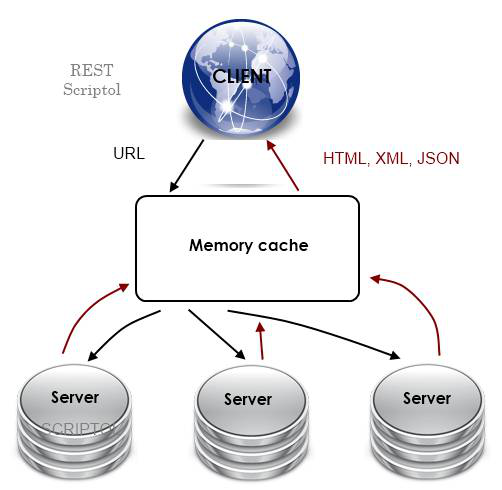
\includegraphics[scale=0.7]{imgs/rest_architecture.png} 
\caption{Modello di architettura REST\label{restimage}}
\end{center}
\end{figure}
\\
Un numero qualsiasi di connettori (client, server, cache, tunnel ecc.) può mediare la richiesta, ma ogni connettore interviene senza conoscere la “storia passata” delle altre richieste(stateless). Di conseguenza una applicazione può interagire con una risorsa conoscendo due cose: l'identificatore della risorsa e l'azione richiesta.
L'applicazione deve conoscere il formato dell'informazione (rappresentazione) restituita, tipicamente un documento HTML, XML o JSON, ma potrebbe essere anche un'immagine o qualsiasi altro contenuto.






\section{Geolocalizzazione}
La geolocalizzazione è l'identificazione della posizione geografica di un dato oggetto nel mondo reale.
Gli oggetti possono essere telefoni cellulari, pc, tablet, palmari e ci sono diverse tecniche, indoor ed outdoor.
\begin{itemize}
\item \textbf{outdoor}: localizzazione satellitare;
\item \textbf{indoor}: infrastrutture ad-hoc e WiFI;
\item \textbf{indoor ed outdoor}: infrastruttura cellulare.
\end{itemize}
Vi sono inolte diversi metodi per valutare la qualità di un sistema di localizzazione:
\begin{itemize}
\item \textbf{Errore medio}: corrispondenza tra la posizione stimata e quella reale;
\item \textbf{Probabilità di corretta locazione}: probabilità di localizzare l'obiettivo entro una determinata soglia;
\item \textbf{Rendimento}: capacità del metodo a stimare la posizione in tutti i tipi di ambienti;
\item \textbf{Consistenza}: misura della stabilità dell'errore medio in ambienti differenti;
\item \textbf{Overhead}: quantità di informazione scambiata tra il terminale ed il sistema;
\item \textbf{Consumo di potenza}: quantita delle risorse energetiche impiegate;
\item \textbf{Latenza}: intervallo di tempo tra la richiesta di posizionamento e la risposta del sistema;
\item \textbf{Costi roll-out}: costi necessari all'installazione dell'infrastruttura;
\item \textbf{Costi operativi}: costi legati al mantenimento dell'infrastruttura.
\end{itemize}

\subsection{Localizzazione satellitare}
La localizzazione satellitare si basa su infrastrutture indipendenti dedicate, ovvero un certo numero di satelliti utilizzati solo a questo scopo e di tipo terminal-based.
I vantaggi del posizionamento satellitare sono la copertura globale e l'alto livello di accuratezza, ma è soggetto anche ad importanti inconvenienti, come un eccessivo consumo dovuto ai dispositivi che utilizzano il segnale GPS e ai disturbi naturali che possono ostacolarne la ricezione.

\subsubsection{GPS}
Il sistema GPS (Global Positioning System)\footnote{Il sito di riferimento per lo standard GPS è \emph{\url{http://www.gps.gov}}.}, avviato dagli USA negli anni '70 e completato nel 1993, è stato realizzato per motivi essenzialmente militari, al fine di consentire il percorso dei mezzi militari, sia sulla terraferma che in mare in modo da localizzarne la posizione in ogni momento e consentire eventuali operazioni di supporto e salvataggio.
Il GPS utilizza dai 24 ai 32 satelliti artificiali, divisi in gruppi da 4, che ruotano attorno alla terra a circa 20.200 km in orbite che formano tra loro angoli di 60 gradi.

\begin{figure}
\begin{center}

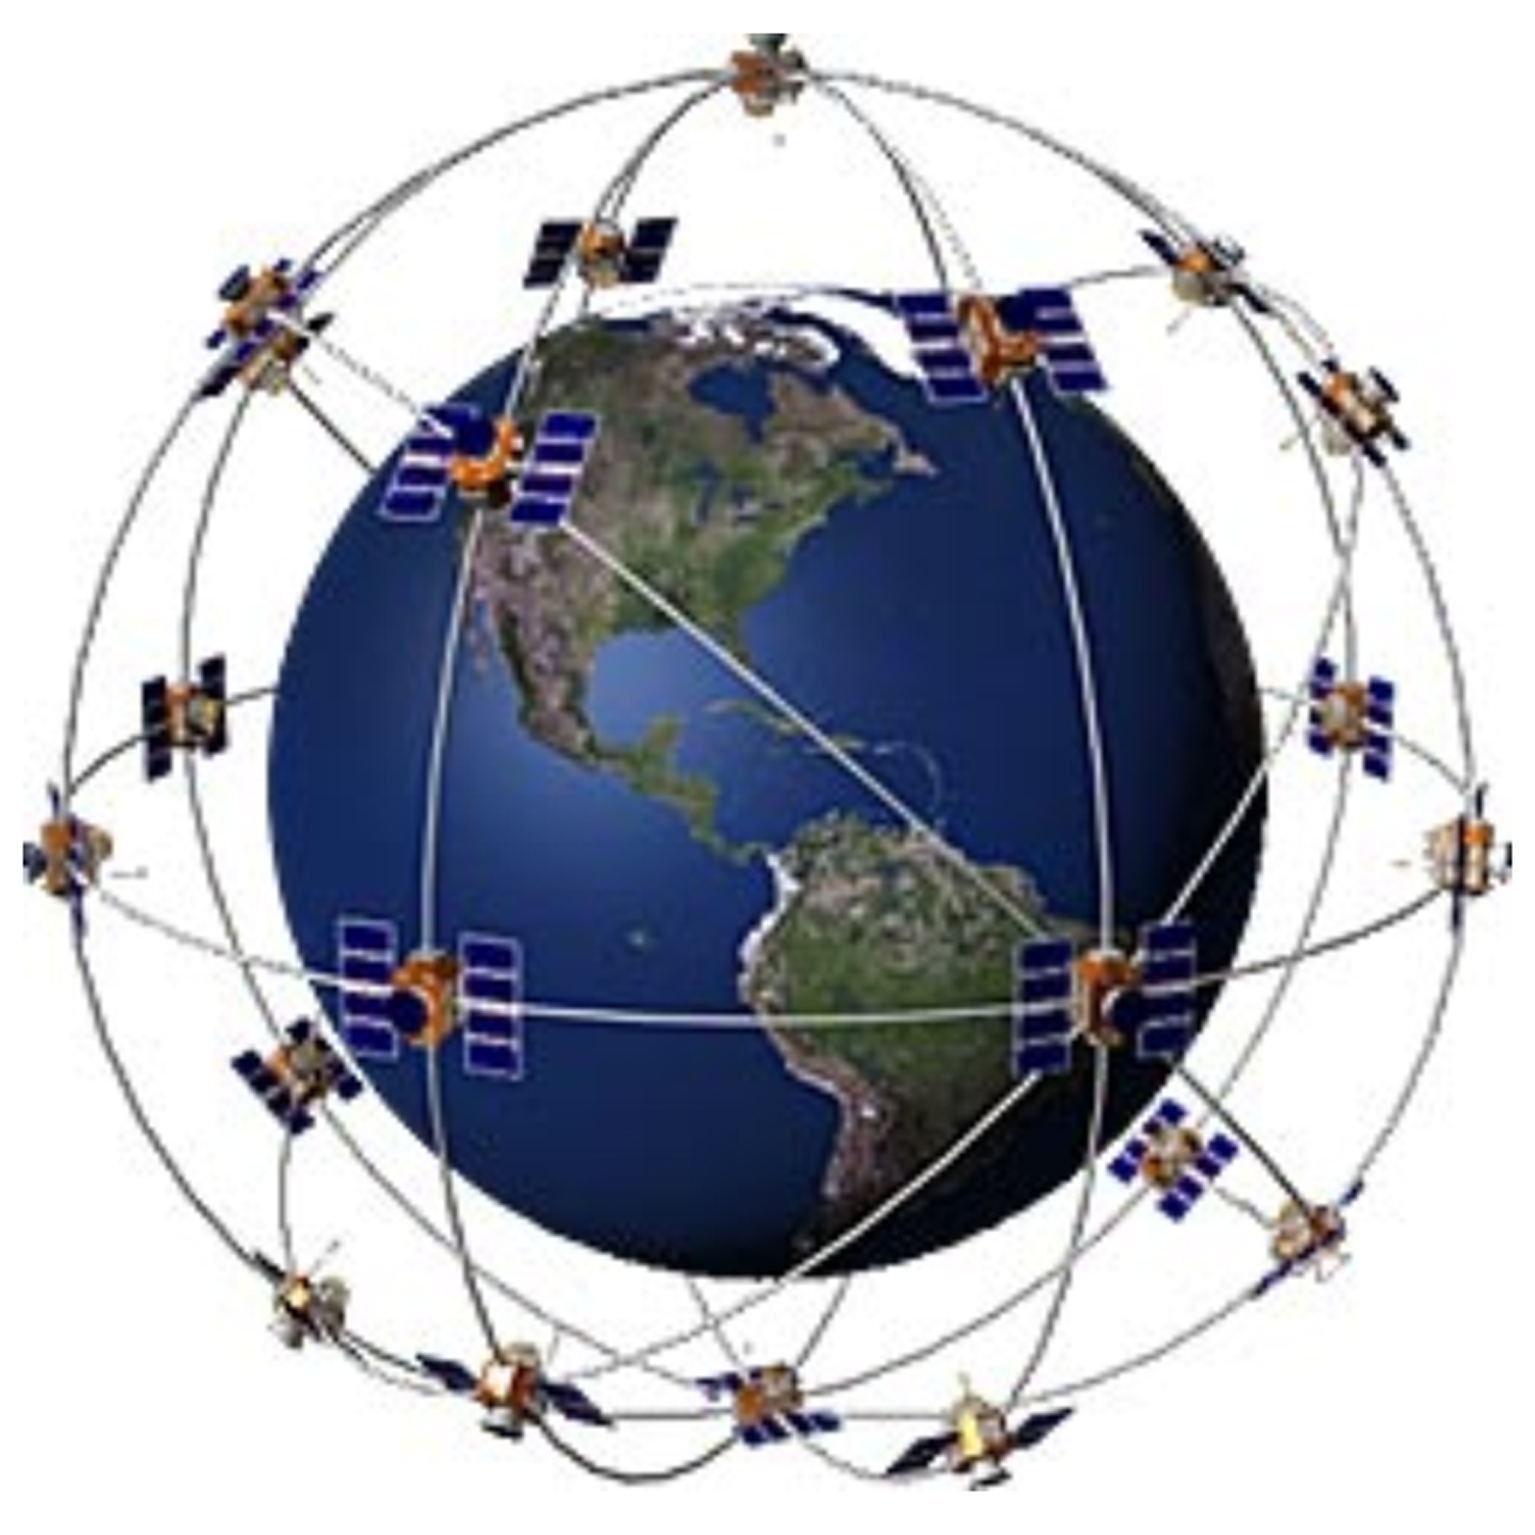
\includegraphics[scale=0.3]{imgs/gpssatelliteimage.jpg}
\caption{Rappresentazione dei satelliti GPS in orbita intorno alla terra\label{gpsimage}}
\end{center}

\end{figure}

\paragraph{Principi di funzionamento}
Il sistema GPS è nato come versione satellitare e perfezionamento del sistema LORAN, nato negli USA attorno al 1940, che consentiva la determinazione della posizione lungo le rotte di grande traffico navale ed aereo, utilizzando un grande numero di stazioni terrestri.

Il sistema GPS, così come il LORAN, consente di determinare la propria posizione sulla superficie terrestre e la propria altitudine in qualunque punto ci si trovi tramite un ricevitore GPS, il quale intercetta a terra il segnale generato dai satelliti in orbita che passano sopra di noi, così come rappresentato in figura \ref{gpsimage}.
Infatti, visto il numero, l'orbita ed il periodo di rotazione, in ogni istante e in ogni punto terreste è possibile intercettare il segnale generato da 6 a 12 satelliti.

\paragraph{Satelliti}
Le funzioni dei satelliti possono essere così sintetizzate:
\begin{itemize}
\item trasmettere informazioni agli utilizzatori mediante un segnale radio;
\item mantenere un riferimento di tempo accurato, grazie agli orologi di bordo;
\item ricevere e memorizzare informazioni dal segmento di controllo;
\item eseguire manovre e correzioni di orbita.
\end{itemize}

\paragraph{Ricevitore}
I ricevitori GPS commerciali, dal costo molto contenuto, consentono di sintonizzarsi automaticamente sulle frequenze dei satelliti GPS e, dopo un tempo di ricerca relativamente breve, di determinare la propria posizione ed, eventualmente, la propria quota, elaborando le distanze di almeno quattro satelliti.
Nei navigatori GPS per auto e negli smartphone, il risultato dell'elaborazione viene mostrato come punto all'interno di una cartina geografica completa, che può essere ingrandita fino a diventare una vera e propria cartina topografica.

\paragraph{Precisione}
La precisione della ricezione GPS è influenzata da una serie di fattori, tra cui la posizione dei satelliti, l'eventuale presenza di rumore del segnale radio, le condizioni atmosferiche e le barriere naturali.
In generale, tali disturbi possono introdurre errori di precisione tra 1 e 10 metri.
La determinazione  più accurata della  posizione si verifica quando il satellite e il ricevitore GPS sono in vista tra loro senza  nessun altro oggetto schermante. Sotto questa ipotesi, il margine di errore del posizionamento è di circa 90 cm.

\subsection{Localizzazione cellulare}
La localizzazione cellulare è utilizzata nelle reti cellulari, come GSM o UMTS, per ricavare la posizione di un utente.
Questo sistema di localizzazione è utilizzato per ricavare la presenza di un utente all'interno di una cella, per cui è soggetto a margini di errore abbastanza ampi.
Per questo motivo, i gestori hanno predisposto nuovi strumenti per equipaggiare le proprie reti con dispositivi e protocolli finalizzati alla realizzazione del posizionamento in modo più accurato ed efficiente.
A tal proposito, diversi metodi sono stati specificati dai gruppi di standardizzazione, come 3GPP (\emph{\url{http://www.3gpp.org}}. La maggior parte di questi metodi è network-based, per cui anche i dispositivi più datati possono usufruirne.
Il vantaggio di questi sistemi di localizzazione cellulare è che possono essere utilizzati anche in ambienti chiusi, diversamente dai sistemi satellitari.
Il posizionamento cellulare può essere molto costoso per quanto riguarda l'overhead dovuto alla segnalazione, soprattutto se è richiesto un alto grado  di accuratezza e, inoltre, la capacità impiegata per la localizzazione è indisponibile per i servizi voce e dati.

\subsection{Localizzazione indoor}
La localizzazione indoor è nata per essere utilizzata all'interno di grandi edifici, campus universitari, strutture museali, strutture ospedaliere e uffici di vario genere.
E' basata su tecnologie radio, infrarossi o ad ultrasuoni, con un raggio di comunicazione evidentemente limitato.
La realizzazione di un sistema di localizzazione indoor può avvenire mediante la realizzazione di infrastrutture dedicate o l'utilizzo di infrastrutture preesistenti, come le reti WLAN.
La localizzazione indoor ha il vantaggio di presentare un basso consumo di potenza dei dispositivi utilizzati per la ricezione e l'elevata accuratezza dovuta al corto raggio delle tecnologie usate.

Esistono diverse soluzioni commerciali per la localizzazione indoor, come \textbf{RADAR} (\emph{\url{http://research.microsoft.com/en-us/projects/radar/}}), sviluppata da Microsoft, che è un sistema a radio frequenza; \textbf{Real Time Location System - RTLS} (\emph{\url{http://www.ekahau.com/real-time-location-system/technology}}), di Ekahau, che si basa sull'infrastruttura WLAN IEEE 802.11; \textbf{Visibility System} (\emph{\url{http://www.aeroscout.com/technology}}), di Aeroscout, basato sempre sull'infrastruttura WLAN IEEE 802.11; \textbf{Wireless Location Appliance} (\emph{\url{http://www.cisco.com/en/US/products/ps6386/index.html}}), di Cisco, basato su WLAN.\\


\section{Web Mapping}
Il Web Mapping è un processo di progettazione, implementazione, generazione e produzione di mappe sul web.
Un caso particolare di mappe web sono le mappe mobili, visualizzate su periferiche mobili, come telefonini, smartphone, tablet e GPS.

I vantaggi derivanti dall'utilizzo di mappe web sono:
\begin{itemize}
\item facilità di generazione di mappe aggiornate;
\item economicità dell'infrastruttura software ed hardware;
\item facilità di distribuzione degli aggiornamenti;
\item supporto e compatibilità con la maggior parte dei browser e dei sistemi operativi;
\item facilità di personalizzazione;
\item supporto per l'hyperlinking di punti di interesse;
\item facilità di integrazione con altri oggetti multimediali.
\end{itemize}

I servizi di web mapping più noti sono \textbf{Google Maps} e \textbf{Bing Maps}.
\subsection{Google Maps}
Google Maps (\emph{\url{https://maps.google.it}}) è un servizio di web mapping nato nel 2005 e fornito da Google, che include numerosi altri servizi basati sulle mappe (mappe stradali, pianificazione di percorsi e localizzazione di imprese).
Le mappe non sono aggiornate in tempo reale, ma spesso dopo mesi o anni.
\subsubsection{Google Maps API}
Google ha messo a disposizione le proprie API per consentire agli sviluppatori di integrare Google Maps all'interno dei loro siti web.
Il servizio offerto è gratuito, anche se Google si riserva, nei termini di licenza, di introdurre future forme di pagamento.

\subsection{Bing Maps}
Bing Maps (\emph{\url{http://it.bing.com/maps/}}) è un servizio di web mapping nato nel 2009 e distribuito da Microsoft nella \textit{Bing suite}.
Fornisce numerose tipologie di mappe: stradali, satellitari, aeree, tridimensionali, oltre che, naturalmente, servizi di traffico e di ricerca delle imprese.
\subsubsection{Bing Maps API}
Microsoft, oltre a mettere a disposizione le Bing API agli sviluppatori, fornisce anche una SDK disponibile su più piattaforme, per realizzare applicazioni integrabili con la maggior parte dei prodotti commerciali Microsoft.



%%%%%%%%%%%%%%%%%%%%%%%%%%%%%%%%%%%%%%%%r%%%%%%%%%%%%%%

\clearpage{\pagestyle{empty}\cleardoublepage}


%%%%%%%%%%%%%%%%%%%%%%%%%%%%%%%%%%%%%%%%%%%%%%%%%%%%%%%%%%%%
% Capitolo 5

\chapter{Tecnologie ed applicativi utilizzati}
\label{tecnologieutilizzate}

Le tecnologie elencate nel capitolo \ref{tecnologie}, sono tutte di interesse applicativo per l'oggetto di questa tesi. Tra esse però, sono state individuate quelle che maggiormente aderiscono agli obiettivi preposti e che, di seguito, verranno elencate e giustificate.
\section{Metodologie di sviluppo agili}
Con il termine \textit{metodologia agile} si intende un insieme di metodi di sviluppo software basati sullo sviluppo iterativo ed incrementale, in cui i requisiti e le soluzioni evolvono attraverso una collaborazione tra team capaci di organizzarsi autonomamente e con esperienze e conoscenze diverse.
Le metodologie agili sono contrapposte alle metodologie \textit{pesanti} e \textit{iterative} poiché promuovono una pianificazione adattabile, uno sviluppo e una consegna del software evolutivi, un approccio iterativo, ed incoraggiano ad una risposta al cambiamento rapida e flessibile.

Le metodologie agili sono state introdotte ufficialmente nel 2001 dal \textit{Manifesto Agile}(\url{http://agilemanifesto.org/}), un documento dell'\textit{Agile Alliance}, l'associazione che ha permesso la diffusione su ampia scala di tali metodologie.
Il Manifesto Agile riporta quanto segue:
\begin{quotation}
We are uncovering better ways of developing software by doing it and helping others do it. Through this work we have come to value:
\begin{itemize}
\item[ ] Individuals and interactions over processes and tools
\item[ ] Working software over comprehensive documentation
\item[ ] Customer collaboration over contract negotiation
\item[ ] Responding to change over following a plan
\end{itemize}
That is, while there is value in the items on the right, we value the items on the left more.
\end{quotation}
I metodi agili quindi preferiscono la comunicazione in tempo reale, preferibilmente faccia a faccia, a quella scritta (documentazione). Il team agile è composto da tutte le persone necessarie per terminare il progetto software. Come minimo il team deve includere i programmatori ed i loro clienti. (Con clienti si intendono le persone che definiscono come il prodotto dovrà essere fatto. Possono essere dei Product Manager, dei Business Analysts, o i clienti finali). L'obiettivo è la piena soddisfazione del cliente e non solo l'adempimento di un contratto. 
L'uso di queste metodologia, inoltre, serve ad abbattere i costi di sviluppo del software e a ridurre al minimo la parte di progettazione che spesso era quella più dispendiosa. Essa è esplosa proprio in concomitanza con la crisi successiva al boom di Internet prendendo spunto dai metodi applicati in piccole software house. Sotto questo nome si raggruppano tecniche come Extreme Programming, SCRUM, Feature Driven Development, DSDM, Disciplined Agile Delivery, Crystal e Lean Software Development.

\subsection{Processi di sviluppo agile}
Così come per i processi di sviluppo tradizionali, anche durante lo sviluppo di software mediante metodologie agili, ci sono delle fasi predefinite: analisi dei requisiti, progettazione, sviluppo e testing. La differenza è che ad ogni iterazione lo sviluppatore ridefinisce e rielabora queste fasi.
I requisiti sono, ad ogni iterazione, approfonditi e migliorati, così come è perfezionato il design. Inoltre è dato molta importanza alla rifattorizzazione, ovvero si modifica la struttura interna di porzioni di codice senza modificarne il comportamento esterno, così da migliorarne la leggibilità ed avere sempre codice di qualità.
Il testing, nell'Agile, riveste un ruolo fondamentale, poiché sono previsti sia gli \textit{Acceptance Test}, ovvero test \textbf{black box} che rappresentano dei risultati attesi dal sistema.
Inoltre vi è il Test Driven Development (TDD), ovvero un modello di sviluppo preceduto dalla stesura di test automatici.

In figura \ref{agiledevelopment} vi è una rappresentazione del processo di sviluppo agile.

\begin{figure}[h!]
\begin{center}
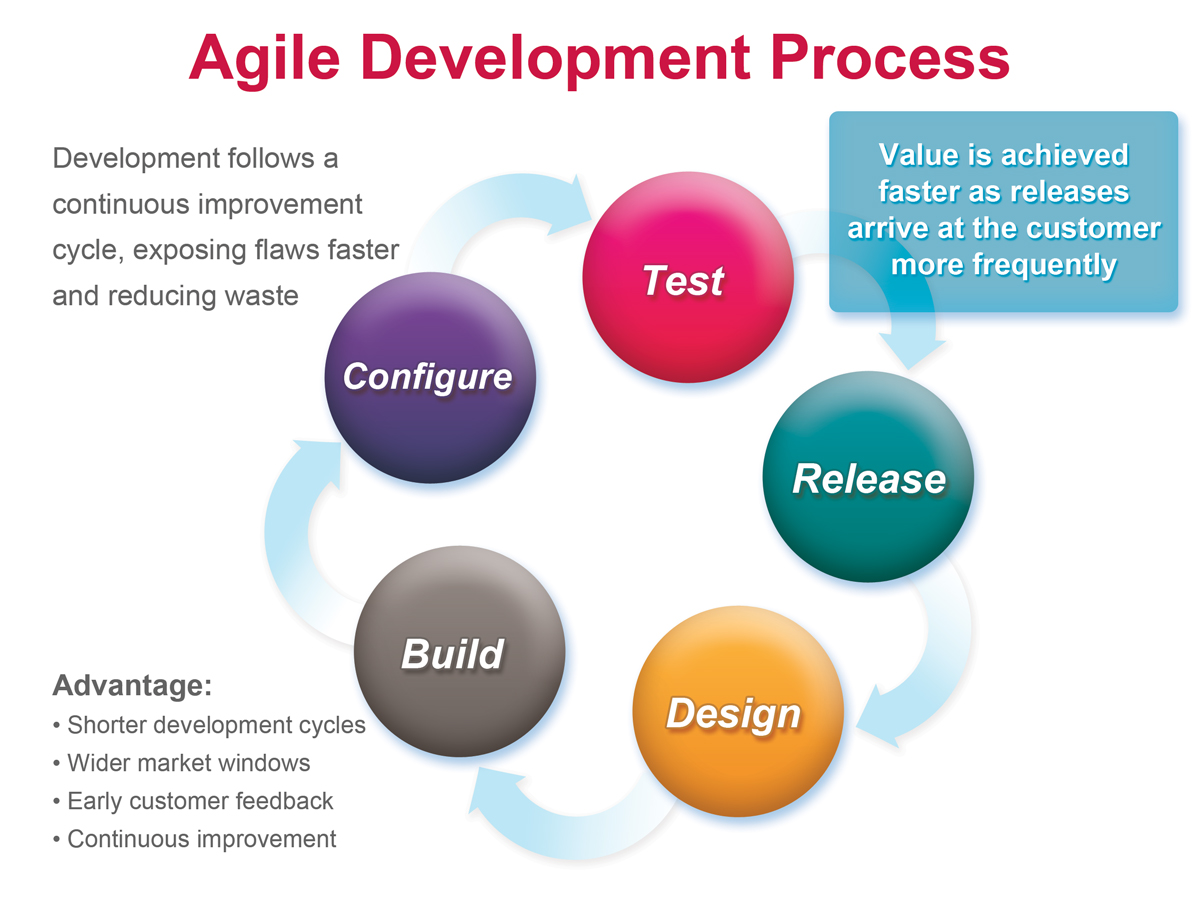
\includegraphics[scale=0.23]{imgs/agiledevelopment.jpg}
\caption{Processo di sviluppo agile\label{agiledevelopment}} 
\end{center}
\end{figure}

La gran parte dei metodi agili tenta di ridurre il rischio di fallimento sia in termini economici, poiché si ha la possibilità di stabilire un tetto di spese limitate che è negoziato frequentemente e monitorato su base costante, sia inteso come forte riduzione del rischio che il cliente si ritrovi in mano funzionalità che non utilizzerà mai o molto raramente. Tutto ciò si può ottenere sviluppando il software in finestre di tempo limitate chiamate \textit{iterazioni} che, in genere, durano qualche settimana.
I fondamenti dei processi agili sono i seguenti:
\begin{itemize}
\item \textbf{iteratività}: prescrive che il processo di sviluppo debba essere ciclico, in modo che le varie fasi siano ripetute più volte in momenti temporali diversi. Questo permette di gestire in modo agile i cambiamenti delle specifiche durante il processo, e non costringe ad aspettare il rilascio del prodotto per poi intraprendere subito una fase di manutenzione, come invece accade con i metodi tradizionali;
\item \textbf{incrementalità}: è il continuo rilascio di versioni parziali del prodotto, le quali inglobano modifiche ed aggiornamenti risultati come necessari alle fasi precedenti. Questo meccanismo permette di rilevare i feedback del committente durante il processo di sviluppo e di adeguare opportunamente il software. In alcuni casi il software rilasciato nelle fasi intermedie è sottoposto anche agli utenti finali, in modo da coglierne le esigenze;
\item \textbf{auto-organizzazione}: il team è lasciato libero di organizzarsi e di adottare di volta in volta le strategie più opportune. Questo favorisce la creatività degli sviluppatori, stimolandoli a trovare soluzioni innovative ai problemi che si presentano;
\item \textbf{emergenza}: bisogna affrontare difficoltà ed imprevisti quando essi si presentano, senza cercare di predeterminarli o una prevenirli. Il principio tradizionale secondo cui un progetto solido deve tener conto dei possibili sviluppi futuri del software viene sovvertito, con la motivazione che si considera inutile spendere tempo e denaro per cercare di prevedere evoluzioni che potrebbero essere disattese.
\end{itemize}
\section{Scelte progettuali}
\subsection{Piattaforma client}
Nell'ambito della localizzazione, la scelta è caduta sulla tecnologia \textbf{GPS}, poichè:
\begin{itemize}
\item \textbf{impossibilità di utilizzo localizzazione indoor}: date le dimensioni considerevoli del sito archeologico, si è ritenuto improbabile l'installazione di una rete WiFi che coprisse tutta l'area, al fine di localizzare tutti i dispositivi presenti;
\item \textbf{inutilità localizzazione cellulare}: la localizzazione cellulare è soggetta a margini di errore ampi per cui, nell'ambito del caso in questione, in cui vi è la necessità di individuare con margini d'errore ridotti la posizione corretta, risulta inutile;
\item \textbf{elevata precisione}: i margini di errore del GPS sono piuttosto bassi, come trattato nel capitolo \ref{tecnologie}.
\end{itemize}


Nella scelta dell'ecosistema su cui sviluppare e presentare un'applicazione per la visita dei siti culturali, \textbf{Windows Phone OS} è stato preferito agli altri, poichè si è tenuto conto di vari fattori:
\begin{itemize}
\item \textbf{originalità}: nello store di Windows Phone, non si trovano applicazioni simili, per cui essa costituirebbe il primo tentativo di visita assistita dei siti culturali;
\item \textbf{utilizzo dispositivi GPS}: l'utilizzo dei dispositivi GPS è molto semplice grazie alle API messe a disposizione da Microsoft. Inoltre si è tenuto conto del background personale.
\end{itemize}

La scelta di Windows Phone OS come piattaforma ha, inoltre, reso quasi obbligatoria l'adozione delle mappe di Bing Maps, che sono supportate nativamente dalla Windows Phone SDK.

\subsection{Piattaforma server}
Il server ospita un application server ed un DBMS.
Il servizio esposto è un \textbf{servizio WCF} (\emph{\url{http://msdn.microsoft.com/en-us/library/dd456779.aspx}}), sviluppato da Microsoft per il trasporto delle informazioni in ambienti distribuiti.
WCF mette assieme le tecnologie di Web Services, Enterprise Service, Message Queuing, fornendo un modello unificato di programmazione per la realizzazione di applicazioni interoperabili.
WCF facilita molto la creazione di un servizio, dal momento che è possibile crearlo ed esporlo tramite IIS (\emph{\url{http://www.iis.net}}) come web service, utilizzando il paradigma REST.

Per la serializzazione dei dati, si è scelto il formato \textbf{GeoRSS} (\emph{\url{http://georss.org}}), un derivato di XML utilizzato specificamente per esportare informazioni georeferenziate.
Un esempio di documento GeoRSS è riportato in figura \ref{georssimage}.
\begin{figure}[h!]
\lstset{language=MYXML}
\begin{lstlisting}
<?xml version="1.0" encoding="utf-8"?>
<feed xmlns="http://www.w3.org/2005/Atom" 
      xmlns:georss="http://www.georss.org/georss" 
      xmlns:gml="http://www.opengis.net/gml">
   <title>Earthquakes</title>
   <subtitle>International earthquake observation labs</subtitle>
   <link href="http://example.org/"/>
   <updated>2005-12-13T18:30:02Z</updated>
   <author>
      <name>Dr. Thaddeus Remor</name>
      <email>tremor@quakelab.edu</email>
   </author>
   <id>urn:uuid:60a76c80-d399-11d9-b93C-0003939e0af6</id>
   <entry>
      <title>M 3.2, Mona Passage</title>
      <link href="http://example.org/2005/09/09/atom01"/>
      <id>urn:uuid:1225c695-cfb8-4ebb-aaaa-80da344efa6a</id>
      <updated>2005-08-17T07:02:32Z</updated>
      <summary>We just had a big one.</summary>
      <georss:point>45.256 -71.92</georss:point>
      </entry>
</feed>
\end{lstlisting}
\caption{Esempio di documento GeoRSS\label{georssimage}}
\end{figure}

Come DMBS si è scelto Sql Server 2012 (\emph{\url{https://www.microsoft.com/italy/server/sql/default.mspx}}), che gestisce al meglio i dati spaziali e su cui c'è la possibilità di utilizzare il framework \textbf{Entity Framework} (\emph{\url{http://msdn.microsoft.com/en-us/data/ef.aspx}}), fornito da \textit{Visual Studio}, trattata di seguito, che consente di creare oggetti a partire dal modello dei dati, al fine di ottenere un alto livello di astrazione.  

\subsection{Ambiente di sviluppo}
In base alle considerazioni ed alle scelte finora effettuate, l'ambiente di sviluppo sarà costituito come di seguito.

\subsubsection{Sistema operativo}
Il sistema operativo utilizzato è Windows 8 (\emph{\url{http://windows.microsoft.com/it-it/windows-8/}}), attualmente il più recente di casa Microsoft.
La scelta è data dalla sua compatibilità con Visual Studio 2012.

\subsubsection{IDE}
L'IDE di sviluppo, in coerenza con le scelte architetturali finora compiute è \textbf{Microsoft Visual Studio} (\emph{\url{http://www.microsoft.com/visualstudio/ita}}), rappresentata con uno screenshot in figura \ref{vsimage}.
Visual Studio permette lo sviluppo di applicazioni console, siti internet, applicazioni grafiche, applicazioni e servizi web, librerie di classi, servizi Windows in tutti i linguaggi di programmazione supportati dal framework .NET, oltre che in tutti i linguaggi di markup, JavaScript e CSS.

\begin{figure}
\begin{center}

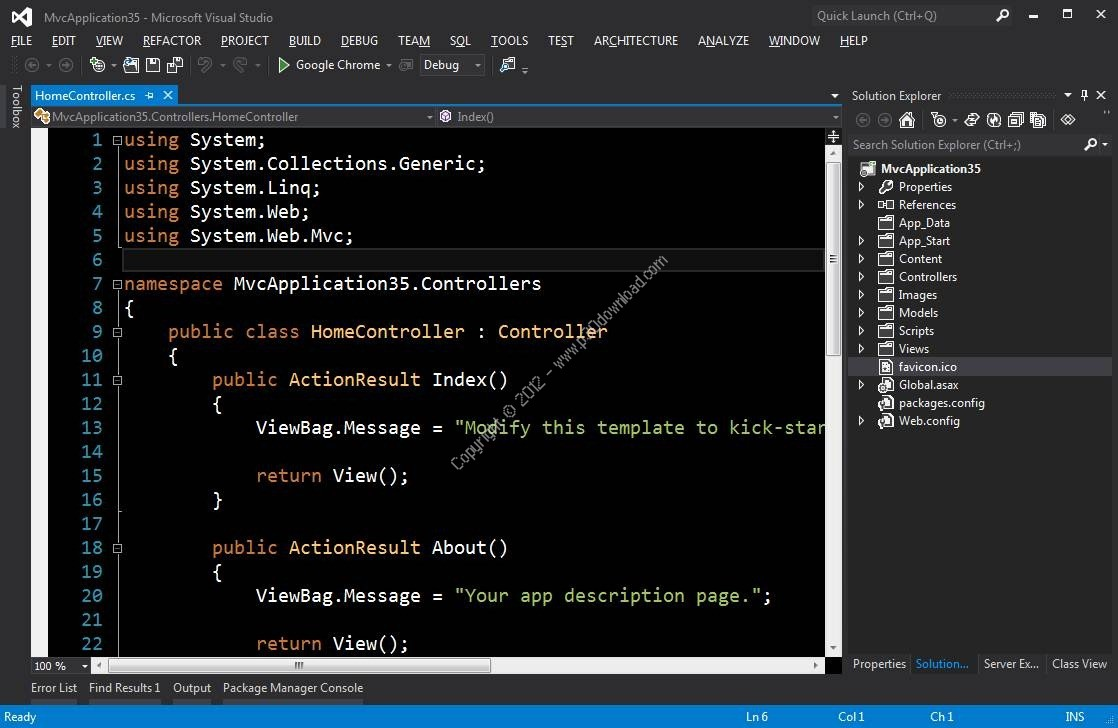
\includegraphics[scale=0.3]{imgs/visualstudio.jpg} 
\caption{Schermata di Visual Studio 2012 Ultimate\label{vsimage}}
\end{center}

\end{figure}
Visual Studio fornisce all’utilizzatore un potente strumento, \textbf{IntelliSense}, che permette
l'autocompletamento del token che il programmatore intende scrivere, oltre che
alla visualizzazione della documentazione e alla gestione delle disambiguità a
video direttamente durante la scrittura del codice.

La versione utilizzata è \textbf{Visual Studio 2012 Ultimate}, lanciata nel settembre 2012.
Essa fornisce numerose nuove features, brevemente elencate:
\begin{itemize}
\item \textbf{Colorazione semantica}: è stata migliorata la colorazione della sintassi, compresi i tipi definiti dall'utente, le macro, i tipi enumerativi e le funzioni;
\item \textbf{Evidenziazione dei riferimenti}: selezione di tutti i riferimenti di un simbolo, una volta selezionato quest'ultimo;
\item \textbf{Nuovo Solution Explorer}: il nuovo Solution Explorer consente agli utenti una visualizzazione per classi o gerarchie di file all'interno del progetto.
E' supportata inoltre la ricerca di chiamate ad una funzione ed utilizzo delle classi;
\item \textbf{Visualizzazione automatica della lista IntelliSense}: IntelliSense è automaticamente visualizzato mentre viene scritto il codice;
\item \textbf{Filtraggio della lista degli elementi}: IntelliSense usa una \textit{fuzzy logic} per determinare quali funzioni/variabili/tipi visualizzare nella lista;
\item \textbf{Code snippets}: è incluso in Intellisense per generare automaticamente frammenti di codice basati sui parametri dell'utente.
\end{itemize}

\subsubsection{Hosting e controllo di versione}
Visual Studio offre, tra i vari servizi, \textbf{Team Foundation Service}, uno strumento di gestione collaborativa del codice che consente di:
\begin{itemize}
\item controllare il proprio codice direttamente in \textit{cloud}, rendendolo accessibile ovunque;
\item gestire il versioning del progetto;
\item gestire la collaborazione nel team;
\item pianificare lo sviluppo agile;
\item gestire il testing e la distribuzione del prodotto.
\end{itemize}



\clearpage{\pagestyle{empty}\cleardoublepage}

%%%%%%%%%%%%%%%%%%%%%%%%%%%%%%%%%%%%%%%%%%%%%%%%%%%%%%%%%%%%
% Capitolo 6

\chapter{Realizzazione del progetto}
\label{progetto}

In questo capitolo verrà discussa l'effettiva realizzazione del progetto, ovvero analisi dei requisiti, progettazione, sviluppo e testing, secondo le metodologie agili.
Ogni progetto inizia con la stesura di un \textit{Project Charter} (Documento di inizio progetto), che, non essendo di interesse in questo contesto, viene qui tralasciato.
Si è proceduto quindi con la definizione delle iterazioni, partendo, naturalmente, dall'\textit{iterazione 0}

\section{Iterazione 0}

Nell'\emph{iterazione 0}, come prassi nelle metodologie agili, vengono realizzate l'analisi dei requisiti, la modellazione delle interfacce utente, la modellazione di dominio e la pianificazione degli incrementi.
L'\emph{iterazione 0} è la base su cui partire per lo sviluppo delle iterazioni successive, perciò ricopre un ruolo fondamentale nello sviluppo Agile.

\subsection{Analisi dei requisiti}
Di seguito sono descritti i requisiti funzionali e non funzionali.

\subsubsection{Requisiti funzionali}
I requisiti funzionali descrivono le funzionalità del sistema software, in termini di servizi che il sistema software deve fornire, di come il sistema software reagisce a specifici tipi di input e di come si comporta in situazioni particolari.
Qui, i requisiti funzionali vengono descritti sotto forma di \textit{user stories}, \textit{epic} (user stories più grandi) e \textit{temi}.

Durante l'analisi è stato individuato un unico tema comune, ovvero:
\begin{itemize}
\item \textit{Gestisci la navigazione assistita del sito}.
\end{itemize}

Da questo tema possiamo ricavare tre \textit{epic}:
\begin{itemize}
\item \textit{Gestisci la mappa del sito};
\item \textit{Gestisci i punti di interesse del sito};
\item \textit{Gestisci l'itinerario del sito}.
\end{itemize}.

Ed, in definitiva, da questi tre epic, possiamo ricavare otto \textit{user stories} che caratterizzano i requisiti dell'applicazione. Tali user stories vengono di seguito riportate, secondo il formato \emph{"essendo un\dots vorrei poter\dots così da\dots"}, comunemente utilizzato:

\begin{itemize}
\item \textit{essendo un utente vorrei poter visualizzare la mia posizione sulla mappa così da orientarmi al meglio all'interno del sito};
\item \textit{essendo un utente vorrei poter visualizzare i punti di interesse sulla mappa così da spostarmi verso di essi};
\item \textit{essendo un utente vorrei poter zoomare e centrare la mappa così da ottenere una visualizzazione migliore};
\item \textit{essendo un utente vorrei poter sapere quando sono vicino ad un punto di interesse così da conoscere informazioni su di esso};
\item \textit{essendo un utente vorrei poter cliccare su un punto di interesse così da conoscere informazioni su di esso};
\item \textit{essendo un utente vorrei poter conoscere i feedback degli altri utenti così da spostarmi verso punti di interesse dal rating noto};
\item \textit{essendo un utente vorrei poter inviare un feedback così da condividere la mia esperienza con gli altri utenti};
\item \textit{essendo un utente vorrei poter ottenere un itinerario così da ottimizzare il tempo di visita}.
\end{itemize}


Per quanto riguarda il servizio, esso deve fornire un file in formato GeoRSS contenente i punti di interesse con le informazioni fondamentali (nome, coordinate spaziali, feedback).

\subsubsection{Requisiti non funzionali}
I requisiti non funzionali descrivono le proprietà del sistema software in relazione a determinati servizi o funzioni e possono anche essere relativi al processo:
\begin{itemize}
\item caratteristiche di efficienza, affidabilità, safety, ecc\dots;
\item caratteristiche del processo di sviluppo (standard di processo, uso di ambienti CASE, linguaggi di programmazione, metodi di sviluppo, ecc\dots);
\item caratteristiche esterne (interoperabilità con sistemi di altre organizzazioni, vincoli legislativi, ecc\dots).
\end{itemize}

Nel caso di sistemi software destinati a dispositivi mobili, vengono introdotte nuove criticità e nuove proprietà da tenere in considerazione che possono essere riassunte in:
\begin{itemize}
\item \textbf{prestazioni}: i dispositivi mobile hanno risorse limitate, in termini di memoria e di potenza di calcolo, per cui le applicazioni devono poter essere eseguite abbastanza efficientemente;
\item \textbf{usabilità}: i dispositivi mobile presentano display dalle dimensioni ridotte, per cui deve essere posta particolare attenzione al design dell'interfaccia;
\item \textbf{funzionalità}: i dispositivi mobile possono avere diverse periferiche (WIFI, GPS, camera), per cui le applicazioni devono tener conto di queste periferiche e bisogna definire il comportamento di esse in caso non fossero presenti tali periferiche;
\item \textbf{connettività}: i dispositivi mobile, in alcune circostanze, possono non avere caratteristiche di connettività (assenza segnale GPS, UMTS o HDSPA, etc\dots) per cui è importante definire il comportamento dell'applicazione in questi casi;
\item \textbf{consumi}:i dispositivi mobile, in quanto alimentati da batterie, sono soggetti a un consumo che dipende anche dalle periferiche utilizzate (WIFI, GPS, flash fotografico, etc\dots).
\end{itemize}

Nello studio dei requisiti della nostra applicazione, si possono definire i requisiti non funzionali di alto livello dell'applicazione client e del server, descritti rispettivamente nelle tabelle in figura \ref{nfrclient} e \ref{nfrserver}.

\begin{figure}[h!]
\begin{center}
\begin{tabular}[c]{|c|p{9cm}|}
\hline
N. & Requisito\\ \hline
1 & L'interfaccia deve essere costituita da una mappa e da una barra di pulsanti\\ \hline
2 & L'applicazione deve impiegare al massimo 10 secondi per l'avvio\\ \hline
3 & L'applicazione deve utilizzare le periferiche disponibili solo quando necessario\\ \hline
4 & L'applicazione deve funzionare con una risoluzione minima di 480x800\\ \hline
5 & L'applicazione deve prevedere una modalità Offline quando non c'è connettività\\ \hline
\end{tabular}
\caption{Requisiti non funzionali dell'applicazione client\label{nfrclient}}
\end{center}
\end{figure}
\begin{figure}[h!]
\begin{center}
\begin{tabular}[c]{|c|p{9cm}|}
\hline
N. & Requisito\\ \hline
1 & Il servizio deve poter funzionare con almeno 10 richieste al secondo\\ \hline
2 & Il servizio deve essere sempre disponibile almeno negli orari di visita del sito\\ \hline
3 & Il servizio deve essere accessibile esclusivamente dai client dell'applicazione\\ \hline
\end{tabular}
\caption{Requisiti non funzionali del server\label{nfrserver}}
\end{center}
\end{figure}


\subsection{Modello di dominio}
Il modello di dominio identifica le entità fondamentali e le relazioni tra esse.
Sono state individuate cinque entità fondamentali:
\begin{itemize}
\item \textbf{Utente}: è la classe che rappresenta l'utilizzatore dell'applicazione. Collabora con le classi Posizione, Feedback;
\item \textbf{Punto di interesse}: è la classe che rappresenta tutte le strutture, i monumenti e le opere d'arte. Ha come caratteristiche intrinseche il nome, un'icona e una url. Collabora con le classi Posizione e Feedback;
\item \textbf{Posizione}: è la classe che definisce il posizionamento di un punto di interesse, in termini di latitudine e longitudine;
\item \textbf{Feedback}: è la classe che definisce il giudizio dato dall'utente. Ha come caratteristiche il voto (in termini numerici), il giudizio e la data;
\item \textbf{Itinerario}: è la classe responsabile di gestire i percorsi. Collabora con la classe Punto di interesse.
\end{itemize}
\begin{figure}
\begin{center}
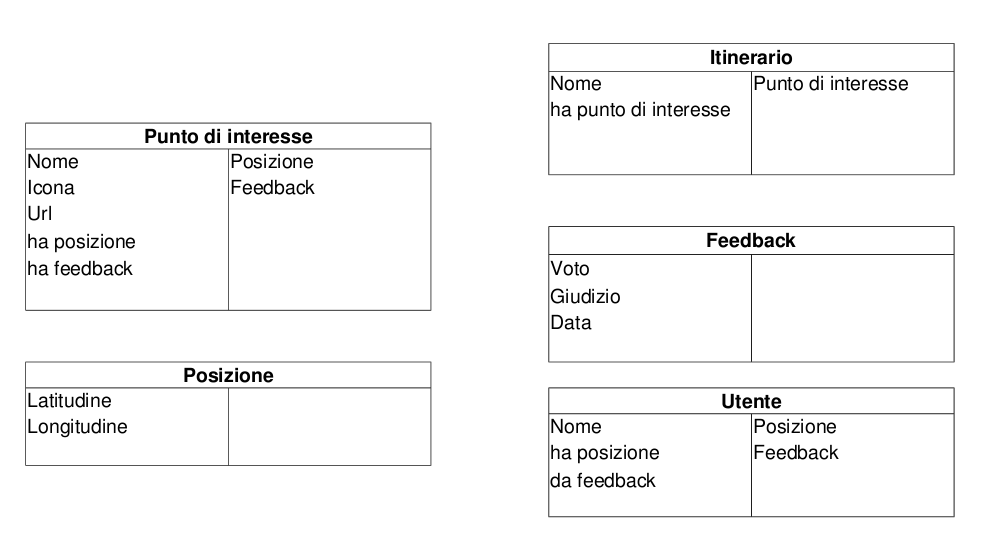
\includegraphics[scale=0.50]{imgs/model/crcmodel.png}
\caption{Modello CRC dell'applicazione\label{crcmodel}}
\end{center}
\end{figure}
Per modellare il dominio vengono qui utilizzate le \textit{Class Responsibility Collaborator (CRC) Cards}, come illustrato in figura \ref{crcmodel}.

\subsection{Modello dell'interfaccia utente}
L'interfaccia utente è la porzione di software che interagisce direttamente con l'utente.
In base ai requisiti non funzionali che caratterizzano l'interfaccia utente, si cerca di realizzare interfacce che tengano conto dell'usabilità.
Vengono riportati di seguito alcuni sketches che costituiscono le schermate dell'applicazione (fig. \ref{sketch}).
\begin{figure}[h!]
\subfloat[Home]{\label{mockuphome}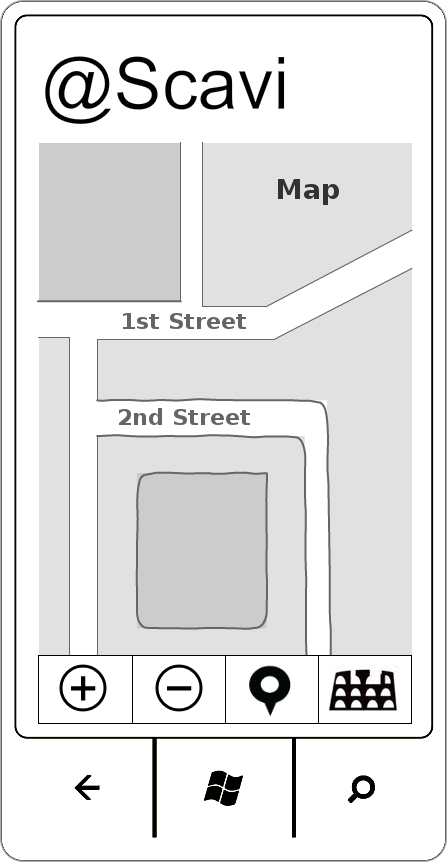
\includegraphics[scale=0.29]{imgs/mockup/home.png}}
\hspace{35mm}
\subfloat[Visualizzazione posizione]{\label{mockupposition}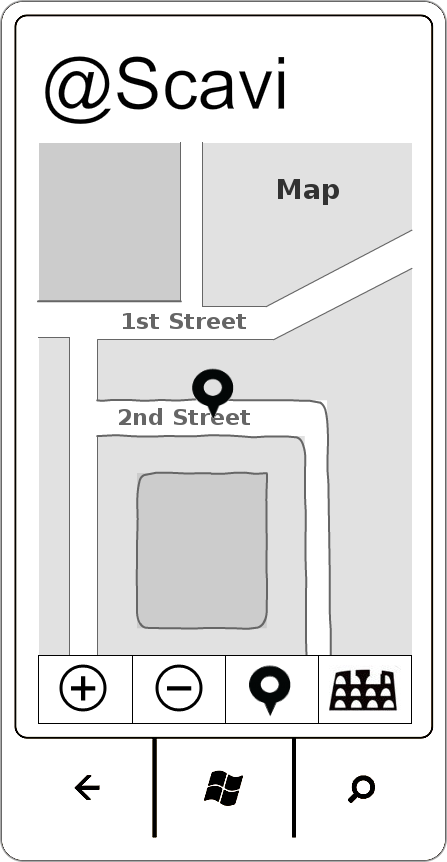
\includegraphics[scale=0.29]{imgs/mockup/position.png}}
 \hspace{35mm}
\subfloat[Visualizzazione punti di interesse]{\label{mockuppushpin}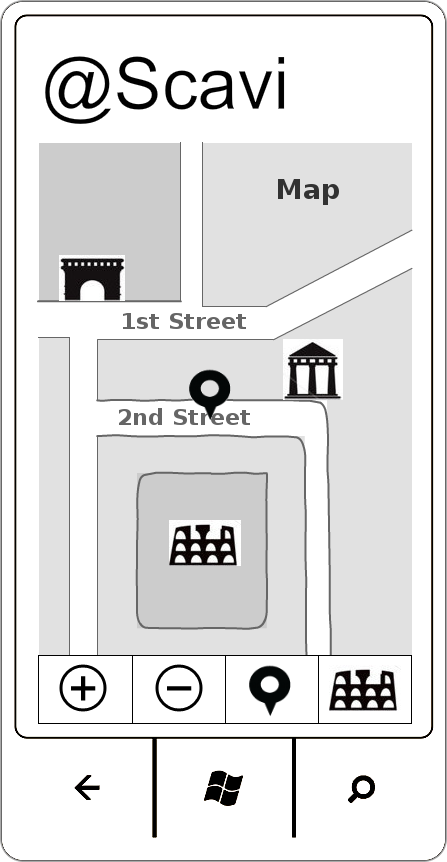
\includegraphics[scale=0.29]{imgs/mockup/pushpin.png}}
 \hspace{35mm}
\subfloat[Visualizzazione menu]{\label{mockuptooltipmenu}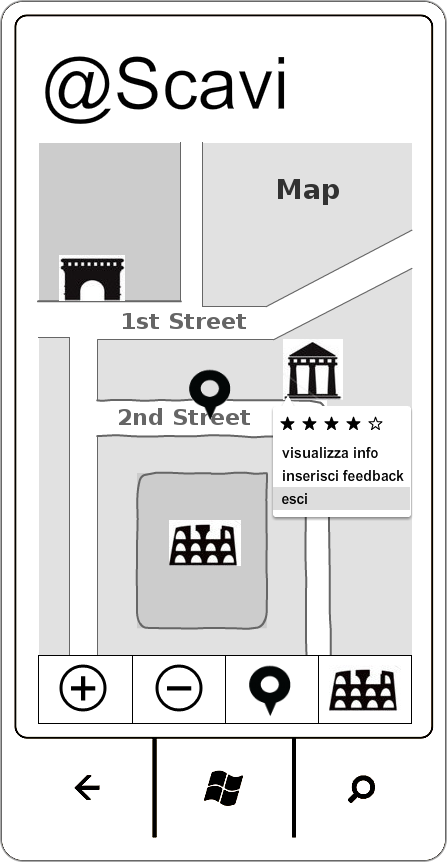
\includegraphics[scale=0.29]{imgs/mockup/tooltipmenu.png}} 
 \hspace{35mm}

\caption{Sketch dell'applicazione, 1\label{sketch}}
\end{figure}

\begin{figure}[h!]
\ContinuedFloat 
\subfloat[Visualizzazione dettaglio]{\label{mockupdetails}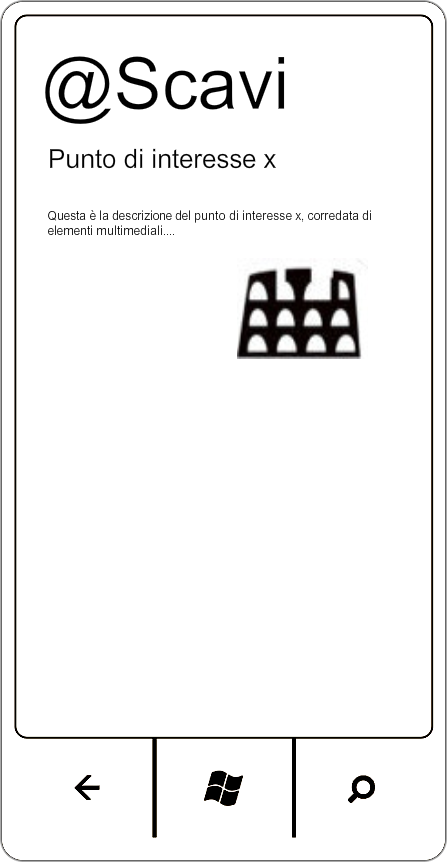
\includegraphics[scale=0.29]{imgs/mockup/details.png}}
 \hspace{35mm}
\subfloat[Invio feedback]{\label{mockupsendfeedback}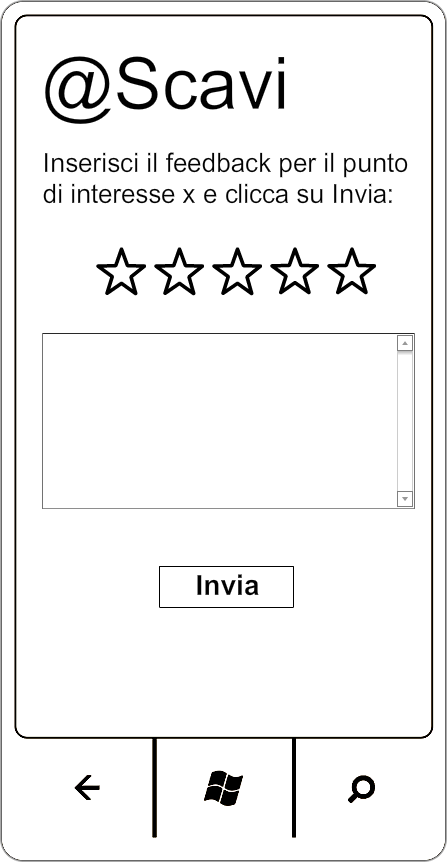
\includegraphics[scale=0.29]{imgs/mockup/sendfeedback.png}}
 \hspace{35mm}

\subfloat[Itinerario]{\label{mockupitinerario}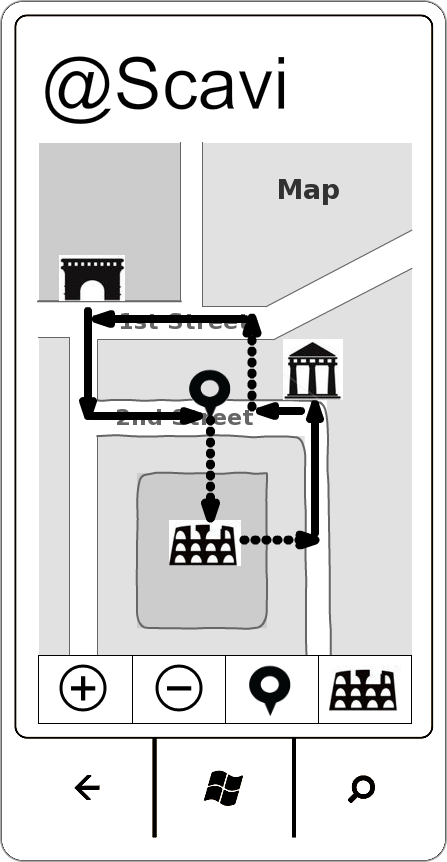
\includegraphics[scale=0.29]{imgs/mockup/route.png}}

\caption{Sketch dell'applicazione, 2\label{sketch}}
\end{figure}

%\Image[width=0.35\linewidth]{imgs/mockup/home.png}{Home}\,
%\Image[width=0.35\linewidth]{imgs/mockup/position.png}{Visualizzazione posizione}
%
%\Image[width=0.35\linewidth]{imgs/mockup/pushpin.png}{Visualizzazione punti di interesse}\,
%\Image[width=0.35\linewidth]{imgs/mockup/tooltipmenu.png}{Visualizzazione menu contestuale}
%
%\Image[width=0.35\linewidth]{imgs/mockup/details.png}{Visualizzazione dettagli} \,
%\Image[width=0.35\linewidth]{imgs/mockup/sendfeedback.png}{Invio feedback}
%
%\Image[width=0.35\linewidth]{imgs/mockup/route.png}{Itinerario}
%\captionof{figure}{Sketch dell'applicazione\label{sketch}}
\clearpage

\subsection{Pianificazione degli incrementi}
Tramite il planning poker\footnote{Il planning poker è una tecnica basata sul consenso per stimare lo sforzo nel completare una user story. E' largamente utilizzata in nelle metodologie agili.}, è stato possibile dare una stima della complessità delle user stories.

\begin{figure}[h!]
\begin{center}
\begin{tabular}[c]{|c|p{7cm}|c|c|}
\hline
N. & User story & Peso & Priorità\\
\hline
1 & \textit{essendo un utente vorrei poter visualizzare la mia posizione sulla mappa così da orientarmi meglio all'interno del sito} & 5 & 10\\
\hline
2 & \textit{essendo un utente vorrei poter visualizzare i punti di interesse sulla mappa così da spostarmi verso di essi} & 8 & 10\\
\hline
3 & \textit{essendo un utente vorrei poter zoomare e centrare la mappa così da ottenere una visualizzazione migliore} & 3 & 9\\
\hline
4 & \textit{essendo un utente vorrei poter sapere quando sono vicino ad un punto di interesse così da conoscere informazioni su di esso} & 5 & 8\\
\hline
5 & \textit{essendo un utente vorrei poter cliccare su un punto di interesse così da conoscere informazioni su di esso} & 3 & 7\\
\hline
6 & \textit{essendo un utente vorrei poter conoscere i feedback degli altri utenti così da spostarmi verso punti di interesse dal rating noto} & 3 & 6\\
\hline
7 & \textit{essendo un utente vorrei poter inviare un feedback così da condividere la mia esperienza con gli altri utenti} & 5 & 5\\
\hline
8 & \textit{essendo un utente vorrei poter ottenere un itinerario così da ottimizzare il tempo di visita} & 15 & 5\\
\hline
\end{tabular}
\caption{Tabella di stima delle user stories\label{userstoriestable}}
\end{center}
\end{figure}
\clearpage

In definitiva abbiamo la tabella in figura \ref{userstoriestable}, con stima e priorità delle user stories.
Considerando una velocità di 15 punti per iterazione e tenendo conto delle priorità, è stato possibile pianificare 3 iterazioni, ciascuna della durata di due settimane, come illustrato in figura \ref{pianificazioneiterazioni}.
Quindi, il progetto verrà sviluppato in sei settimane.
\begin{figure}[h!]
\begin{center}

\begin{tabular}[c]{|c|p{7cm}|c|c|}
\hline
Iterazione & User story\\ \hline
\textbf{Prima iterazione} & 1,2,3 \\ \hline
\textbf{Seconda iterazione} & 4,5,6,7\\ \hline
\textbf{Terza iterazione} & 8\\ \hline
\end{tabular}
\caption{Pianificazione delle iterazioni\label{pianificazioneiterazioni}}

\end{center}
\end{figure}

\clearpage

\section{Iterazione 1}
Nelle iterazione 1 viene effettuata l'analisi dei requisiti per tutti i requisiti corrispondenti alle user stories che ne fanno parte; vengono esplicitati i casi di test; vengono sviluppati alcuni modelli, in particolare i modelli strutturali (modello dei dati e diagramma delle classi) e i modelli comportamentali (diagramma di sequenza), migliorando e ridefinendo, se necessario, i modelli dell'iterazione precedente; vengono, inoltre, mostrati alcuni dettagli di implementazione corrispondenti a porzioni di codice; infine vengono mostrati gli screenshot dell'applicazione.\\

\subsection{Analisi dei Requisiti}
Nell'analisi dei requisiti, le \textit{user stories} vengono suddivise in task; i requisiti non funzionali vengono validati, migliorati e approfonditi.

%Gli sketch della prima iterazione sono quelli in figura \ref{sketch1iterazione}.
%\begin{figure}
%\subfigure[prima]{ 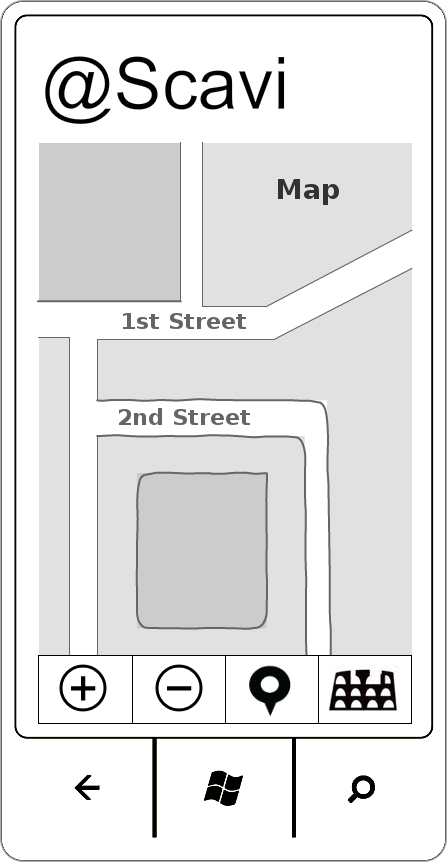
\includegraphics[scale=0.29]{imgs/mockup/home.png} }
%\subfigure[seconda]{ 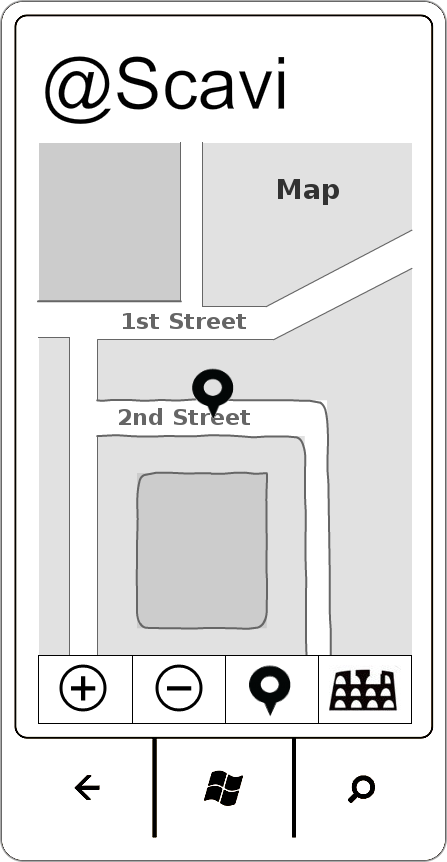
\includegraphics[scale=0.29]{imgs/mockup/position.png} }
%\subfigure[terza]{ 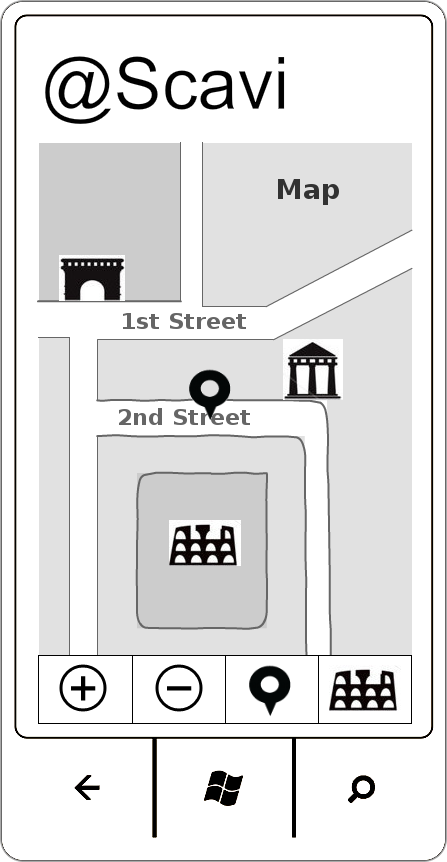
\includegraphics[scale=0.29]{imgs/mockup/pushpin.png} }
%\caption{Sketch della prima iterazione, I\label{sketch1iterazione}}
%\end{figure}
\subsubsection{Requisiti funzionali}
In questa iterazione, come già specificato prima, sono sviluppate le user stories 1,2 e 3 (fig. \ref{userstoriestableprimaiterazione}). \\
\begin{figure}[h!]
\begin{center}
\begin{tabular}[c]{|c|p{7cm}|c|c|}
\hline
N. & User story & Peso & Priorità\\
\hline
1 & \textit{essendo un utente vorrei poter visualizzare la mia posizione sulla mappa così da orientarmi meglio all'interno del sito} & 5 & 10\\
\hline
2 & \textit{essendo un utente vorrei poter visualizzare i punti di interesse sulla mappa così da spostarmi verso di essi} & 8 & 10\\
\hline
3 & \textit{essendo un utente vorrei poter zoomare e centrare la mappa così da ottenere una visualizzazione migliore} & 3 & 9\\
\hline
\end{tabular}
\caption{Tabella di stima delle user stories della prima iterazione\label{userstoriestableprimaiterazione}}
\end{center}
\end{figure}
\clearpage

Considerando le tre user stories, possiamo definire i seguenti task che caratterizzeranno la prima iterazione:\\
\textbf{Lato client}
\begin{itemize}
\item \textbf{creazione form con mappa e pulsanti di utility};
\item \textbf{visualizzazione posizione sulla mappa};
\item \textbf{visualizzazione punti di interesse sulla mappa};
\item \textbf{interfacciamento col dispositivo GPS};
\item \textbf{connessione al un servizio esterno};
\item \textbf{gestione dei layer della mappa}.
\end{itemize}

\textbf{Lato server}
\begin{itemize}
\item \textbf{mapping della base di dati};
\item \textbf{esportazione nel formato GeoRss}.
\end{itemize}

\subsubsection{Requisiti non funzionali}
I requisiti non funzionali già individati per questa prima iterazione sono presenti nella tabella in fig. \ref{nfrclient}.
Dopo un'analisi delle user stories e delle criticità presenti, possiamo individuare altri requisiti non funzionali:
\begin{itemize}
\item L'applicazione deve conservare i dati scaricati per la consultazione offline;
\item I punti di interesse devono avere icone diverse a seconda della tipologia;
\item La mappa deve essere centrata subito dopo la ricezione della posizione;
\item L'applicazione deve gestire l'assenza, la disattivazione e il mancato funzionamento delle periferiche GPS e di rete.
\end{itemize}

Per quanto riguarda il servizio, oltre ai requisiti già individuati nella tabella in fig. \ref{nfrserver}, definiamo il seguente requisito:
\begin{itemize}
\item Il servizio deve generare un file dal formato GeoRss conforme con gli standard di W3C.
\end{itemize}



\subsection{Casi di Test}
Durante l'analisi dei requisiti funzionali e non funzionali, è scaturito che particolare attenzione va posta, in questa fase, allo scambio dei dati col server ed alle periferiche di posizionamento e di rete.
Sono quindi sviluppati i seguenti test di accettazione:
\begin{enumerate}
\item Verificare l'avvio dell'applicazione.
\begin{enumerate}
\item Chiudere i dispositivi di rete o chiudere la connessione dati. \\Avviare l'applicazione. \\Verificare il messaggio di allerta che indica l'assenza di connessione dati e chiede di cliccare per aprire la form delle propietà di connessione.
\begin{enumerate}
\item Verificare la possibilità di chiudere il messaggio di allerta.
\item Verificare che cliccando si apra la form delle proprietà di connessione.
\item Verificare il reloading della schermata iniziale dell'applicazione con le nuove impostazioni.
\item Verificare il nuovo messaggio di alert nel caso non vi sia ancora connettività.
\end{enumerate}

\item Attivare i dispositivi di rete. \\Assicurarsi della presenza di una connessione dati attiva. \\Avviare l'applicazione. \\Verificare l'avvio della schermata principale con mappa e barra dei pulsanti di utility.
\begin{enumerate} 
\item Verificare la possibilità di cliccare e spostarsi sulla mappa.
\end{enumerate}
\end{enumerate}

\item Verificare il funzionamento del pulsante di posizionamento.
\begin{enumerate}
\item Spegnere il dispositivo di puntamento o assicurarsi di mancanza di ricezione del segnale GPS. \\Cliccare sul pulsante per ottenere la posizione attuale. \\Verificare il messaggio di allerta che indica l'assenza di dispositivi di posizionamento e chiede di cliccare per aprire la form delle propietà del GPS. 
\begin{enumerate}
\item Verificare la possibilità di chiudere il messaggio di allerta.
\item Verificare che cliccando si apra la form delle proprietà del posizionamento.
\item Nel caso siano stati attivati dispositivi di puntamento, verificare l'aggiornamento automatico della mappa alla posizione corrente.
\end{enumerate}
\item Attivare il dispositivo GPS e assicurarsi della ricezione del segnale GPS. \\Cliccare sul pulsante per ottenere la posizione attuale. \\Verificare che sulla mappa venga segnalata la posizione attuale.
\begin{enumerate}
\item Verificare che la mappa venga centrata sulla posizione attuale
\end{enumerate}
\end{enumerate}

\item Verificare il funzionamento del pulsante di visualizzazione dei punti di interesse.
\begin{enumerate}
\item Chiudere i dispositivi di rete o chiudere la connessione dati. \\Cliccare sul pulsante di visualizzazione dei punti di interesse.\\ Verificare il messaggio di allerta che indica l'assenza di connessione dati e chiede di cliccare per aprire la form delle propietà di connessione.
\begin{enumerate}
\item Verificare la possibilità di chiudere il messaggio di allerta.
\item Verificare che cliccando si apra la form delle proprietà di connessione.
\item Verificare il reloading della mappa con le nuove impostazioni e, nel caso vi sia connessione dati attiva, la visualizzazione dei punti di interesse.
\end{enumerate}

\item Attivare i dispositivi di rete. \\Assicurarsi della presenza di una connessione dati attiva. \\Cliccare sul pulsante di visualizzazione dei punti di interesse. \\Porre in ingresso uno stream di dati GeoRss valido.
\begin{enumerate}
\item Verificare visualizzazione punti di interesse sulla mappa
\end{enumerate}

\item Attivare i dispositivi di rete. \\Assicurarsi della presenza di una connessione dati attiva. \\Cliccare sul pulsante di visualizzazione dei punti di interesse. \\Porre in ingresso uno stream di dati GeoRss non valido, incompleto o nullo. \\Verificare il messaggio di allerta che indica l'errato parsing del file.
\begin{enumerate}
\item Verificare la possibilità di chiudere il messaggio di allerta.
\item Verificare il ritorno alla visualizzazione precedente.
\end{enumerate}
\item Attivare i dispositivi di rete.\\Assicurarsi della presenza di una connessione dati attiva.\\Cliccare sul pulsante di visualizzazione dei punti di interesse. \\Rendere inaccessibile il servizio per lo stream dei dati GeoRss.\\Verificare il messaggio di allerta che indica la mancata accessibilità del servizio.
\begin{enumerate}
\item Verificare la possibilità di chiudere il messaggio di allerta.
\item Verificare il ritorno alla visualizzazione precedente.
\end{enumerate}
\end{enumerate}
\item Cliccare sui pulsanti di zoom. \\Verificare l'ingrandimento o la riduzione della scala della mappa.
\end{enumerate}


\subsection{Modellazione}
\subsubsection{Modelli strutturali}
\paragraph{Modello dei dati}
\subparagraph{Client}
Nell'iterazione 1, il client gestisce tre tipologie di dati:
\begin{itemize}
\item \textbf{Punto di interesse}
\item \textbf{Tipologia}
\item \textbf{Posizione}
\end{itemize}
Per cui abbiamo un modello dei dati che può essere sintetizzato come in fig. \ref{datamodel1iterazione}.
\begin{figure}
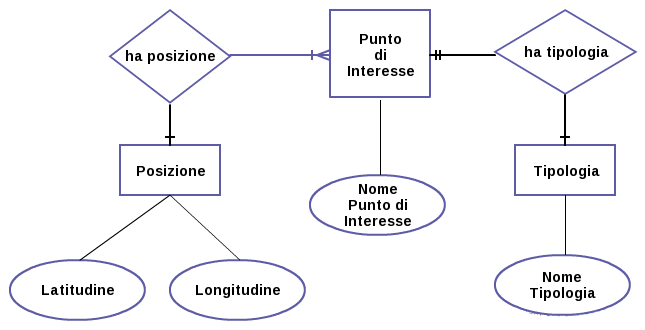
\includegraphics[scale=0.55]{imgs/model/DataModel1.png} 
\caption{Modello dei dati prima iterazione\label{datamodel1iterazione}}
\end{figure}

\paragraph{Diagramma delle classi}

\subsubsection{Modelli comportamentali}
\paragraph{Diagramma di sequenza}
\subsection{Implementazione}

\subsection{Screenshot}





\clearpage

\section{Iterazione 2}

\subsection{Analisi dei requisiti}

\subsubsection{Requisiti funzionali}
Nell'iterazione 2 sono sviluppate le user stories 4,5,6 e 7 (fig. \ref{userstoriestablesecondaiterazione}). 
\begin{figure}
\begin{center}
\begin{tabular}[c]{|c|p{7cm}|c|c|}
\hline
N. & User story & Peso & Priorità\\
\hline
4 & \textit{essendo un utente vorrei poter sapere quando sono vicino ad un punto di interesse per poter conoscere informazioni su di esso} & 5 & 8\\
\hline
5 & \textit{essendo un utente vorrei poter cliccare su un punto di interesse per poter conoscere informazioni su di esso} & 3 & 7\\
\hline
6 & \textit{essendo un utente vorrei poter conoscere i feedback degli altri utenti per poter spostarmi verso punti di interesse dal rating noto} & 3 & 6\\
\hline
7 & \textit{essendo un utente vorrei poter inviare un feedback per condividere la mia esperienza con gli altri utenti} & 5 & 5\\
\hline
\end{tabular}
\caption{Tabella di stima delle user stories della seconda iterazione\label{userstoriestablesecondaiterazione}}
\end{center}
\end{figure}

Considerando queste quattro user stories, possiamo definire i seguenti task che caratterizzano la seconda iterazione:\\
\textbf{Lato client}
\begin{itemize}
\item \textbf{realizzazione form per visualizzazione di informazioni sul punto di interesse};
\item \textbf{realizzazione servizio per la gestione della posizione sulla mappa};
\item \textbf{connessione al servizio di lettura feedback};
\item \textbf{menu contestuale con visualizzazione feedback};
\item \textbf{connessione al servizio di scrittura feedback};
\item \textbf{realizzazione form per inserimento feedback}.
\end{itemize}

\textbf{Lato server}
\begin{itemize}
\item \textbf{creazione servizio per la lettura dei feedback};
\item \textbf{creazione servizio per la scrittura dei feedback}.
\end{itemize}


\subsubsection{Requisiti non funzionali}
Oltre ai requisiti non funzionali già elencati, per l'applicazione si aggiungono i seguenti requisiti:
\begin{itemize}
\item L'applicazione deve gestire la situazione in cui la distanza da due o più punti di interesse sia uguale.
\item L'applicazione deve gestire localmente la vicinanza ai punti di interesse.
\item L'utente può inviare feedback anonimamente.
\item L'utente può inviare al massimo un feedback per ogni punto di interesse.
\item Il commento di feedback deve essere contenuto nei 1000 caratteri.
\end{itemize}

Per il server, invece si può aggiungere:
\begin{itemize}
\item Il sistema deve generare un codice hash per ogni utente.
\end{itemize}



\subsection{Casi di Test}
Dopo l'analisi dei requisiti funzionali e non funzionali, sono stati sviluppati i seguenti casi di test:
\begin{enumerate}
\item Verificare visualizzazione automatica informazioni sul punto di interesse
\begin{enumerate}
\item Assicurarsi che sulla mappa siano visibili i punti di interesse.\\
Assicurarsi della presenza del segnale GPS.\\
Assicurarsi della presenza di una connessione dati attiva.\\
Avvicinarsi fisicamente ad un punto di interesse.\\
\begin{enumerate}
\item Verificare la visualizzazione sul display di informazioni sul punto di interesse.
\item Verificare la possibilità di ritornare alla schermata precedente.
\end{enumerate}
\end{enumerate}
\item Verificare visualizzazione informazioni sul punto di interesse tramite click
\begin{enumerate}
\item Assicurarsi che sulla mappa siano visibili i punti di interesse.\\
Assicurarsi della presenza di una connessione dati attiva.\\
Cliccare sull'icona rappresentante il punto di interesse scelto.
\begin{enumerate}
\item Verificare la visualizzazione di un popup con una voce "visualizza info".
\item Verificare la possibilità di cliccare sulla voce "visualizza info".
\item Verificare la visualizzazione delle informazioni riguardanti il punto di interesse cliccato.
\item Verificare la possibilità di tornare alla schermata precedente.
\end{enumerate}
\end{enumerate}
\item Verificare visualizzazione feedback
\begin{enumerate}
\item Assicurarsi che sulla mappa siano visibili i punti di interesse.\\
Assicurarsi della presenza di una connessione dati attiva.\\
Cliccare sull'icona rappresentante il punto di interesse scelto.
\begin{enumerate}
\item Verificare la visualizzazione di un popup.
\item Verificare la presenza, nella parte superiore del popup, di cinque stelle, colorate a seconda del rating.
\item Verificare la possibilità di tornare alla schermata precedente.
\end{enumerate}
\end{enumerate}
\item Verificare invio feedback
\begin{enumerate}
\item Assicurarsi che sulla mappa siano visibili i punti di interesse.\\
Assicurarsi della presenza di una connessione dati attiva.\\
Cliccare sull'icona rappresentante il punto di interesse scelto.
\begin{enumerate}
\item Verificare la visualizzazione di un popup con una voce "inserisci feedback".
\item Verificare la possibilità di cliccare sulla voce "inserisci feedback".
\item Verificare la visualizzazione sul display di un form perd l'inserimento del feedback.
\item Verificare la possibilità di cliccare sul controllo contenete le cinque stelle.
\item Verificare la possibilità di inserire contenuti nella casella testo.
\item Verificare la possibilità di premere il pulsante "invia" per inviare il feedback.
\end{enumerate}
\end{enumerate}
\end{enumerate}


\subsection{Modellazione}
\subsubsection{Modelli strutturali}
\paragraph{Modello dei dati}
\subparagraph{Client}
Nell'iterazione 1, il client gestisce tre tipologie di dati:
\begin{itemize}
\item \textbf{Punto di interesse}
\item \textbf{Tipologia}
\item \textbf{Posizione}
\end{itemize}
Per cui abbiamo un modello dei dati che può essere sintetizzato come in fig. \ref{datamodel1iterazione}.
\begin{figure}
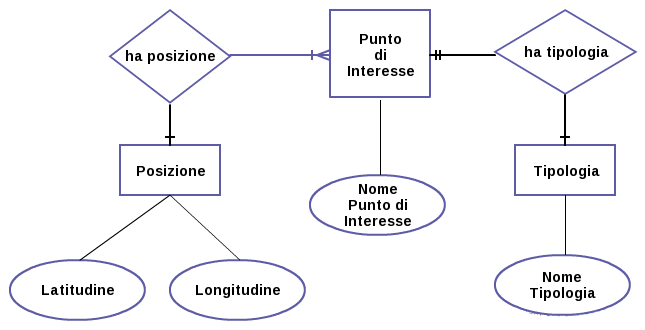
\includegraphics[scale=0.55]{imgs/model/DataModel1.png} 
\caption{Modello dei dati prima iterazione\label{datamodel1iterazione}}
\end{figure}

\paragraph{Diagramma delle classi}

\subsubsection{Modelli comportamentali}
\paragraph{Diagramma di sequenza}
\subsection{Implementazione}

\subsection{Screenshot}


\clearpage

\section{Iterazione 3}

\subsection{Analisi dei requisiti}
\subsubsection{Requisiti funzionali}
Nell'iterazione 3 è sviluppata la user story 8 (fig. \ref{userstoriestableterzaiterazione}). 
\begin{figure}[h!]
\begin{center}
\begin{tabular}[c]{|c|p{6cm}|c|c|}
\hline
N. & User story & Peso & Priorità\\
\hline
8 & \textit{essendo un utente vorrei poter ottenere un itinerario per poter ottimizzare il tempo di visita} & 15 & 5\\
\hline
\end{tabular}
\caption{Tabella di stima delle user stories della terza iterazione\label{userstoriestableterzaiterazione}}
\end{center}
\end{figure}

Considerando tale user story, possiamo definire i seguenti task che caratterizzano la terza iterazione:\\
\textbf{Lato client}
\begin{itemize}
\item \textbf{realizzazione form per visualizzazione dell'itinerario};
\item \textbf{connessione al servizio per la gestione della posizione}.
\end{itemize}

\textbf{Lato server}
\begin{itemize}
\item \textbf{realizzazione servizio per la gestione della posizione};
\item \textbf{realizzazione servizio per la creazione del feedback}.
\end{itemize}

\subsubsection{Requisiti non funzionali}
Oltre ai requisiti non funzionali già descritti nelle precedenti iterazioni, per le funzionalità previste in questa fase, si può aggiungere:
\begin{itemize}
\item L'itinerario deve tener conto della posizione dell'utente ed indicare la direzione
\item L'utente deve poter conoscere in ogni momento la distanza mancante alla fine dell'itinerario.
\end{itemize}

\subsection{Casi di Test}
\subsection{Modellazione}
\subsubsection{Modelli strutturali}
\paragraph{Modello dei dati}
\subparagraph{Client}
Nell'iterazione 1, il client gestisce tre tipologie di dati:
\begin{itemize}
\item \textbf{Punto di interesse}
\item \textbf{Tipologia}
\item \textbf{Posizione}
\end{itemize}
Per cui abbiamo un modello dei dati che può essere sintetizzato come in fig. \ref{datamodel1iterazione}.
\begin{figure}
\includegraphics[scale=0.55]{imgs/model/DataModel1.png} 
\caption{Modello dei dati prima iterazione\label{datamodel1iterazione}}
\end{figure}

\paragraph{Diagramma delle classi}

\subsubsection{Modelli comportamentali}
\paragraph{Diagramma di sequenza}
\subsection{Implementazione}
\subsection{Screenshot}

\clearpage
%%%%%%%%%%%%%%%%%%%%%%%%%%%%%%%%%%%%%%%%%%%%%%%%%%%%%%

\clearpage{\pagestyle{empty}\cleardoublepage}

%%%%%%%%%%%%%%%%%%%%%%%%%%%%%%%%%%%%%%%%%%%%%%%%%%%%%%%%%%%%
% Capitolo ??

\chapter*{Conclusioni}
\label{ref:conclusioni}




\clearpage{\pagestyle{empty}\cleardoublepage} \addcontentsline{toc}{chapter}{Conclusioni}
\appendix
%%%%%%%%%%%%%%%%%%%%%%%%%%%%%%%%%%%%%%%%%%%%%%%%%%%%%%%%%%%%

\chapter{Appendice}
\label{ref:appendice}


Nella presente appendice saranno esposte le porzioni di codice di particolare interesse ai fini della realizzazione dell'applicazione.
\subsubsection{Connessione al GPS}
Nella figura\ref{GPSConnection} è mostrato come il client è interfacciato al dispositivo GPS.
\begin{figure}
\begin{center}
\lstset{language=CSharp}
\begin{lstlisting}
async Task<GeoCoordinate> GetPosition()
        {
            if ((bool)IsolatedStorageSettings.ApplicationSettings["LocationConsent"] != true)
            {
                MessageBox.Show("Attivare i servizi di posizionamento");
            }

            Geolocator geolocator = new Geolocator();
            geolocator.DesiredAccuracyInMeters = 50;

            try
            {
                Geoposition geoposition = await geolocator.GetGeopositionAsync(
                    maximumAge: TimeSpan.FromMinutes(5),
                    timeout: TimeSpan.FromSeconds(10)
                    );

                GeoCoordinate coordinateToBack = new GeoCoordinate();
                coordinateToBack.Latitude = geoposition.Coordinate.Latitude;
                coordinateToBack.Longitude = geoposition.Coordinate.Longitude;
                return coordinateToBack;
            }
            catch (ArgumentException AE)
            {
                MessageBox.Show(AE.StackTrace);
            }
        }
\end{lstlisting}
\caption{Gestione della connessione al dispositivo GPS\label{GPSConnection}}
\end{center}
\end{figure}


\clearpage
%%%%%%%%%%%%%%%%%%%%%%%%%%%%%%%%%%%%%%%%%%%%%%%%%%%%%%

\clearpage{\pagestyle{empty}\cleardoublepage}
%%%%\clearpage{\pagestyle{empty}\cleardoublepage}

\end{mainmatter}

\begin{backmatter}


\begin{thebibliography}{9}
\bibitem[argomento]{etichetta} Cognome, N., \emph{Titolo}, Editore, Luogo, Data, ecc.
\end{thebibliography}

\clearpage{\pagestyle{empty}\cleardoublepage}
 
\addcontentsline{toc}{chapter}{Sitografia}

\begin{thesitography}{9}
\bibitem{www:DATABENC} http://www.databenc.it/
\bibitem{www:ancitel} http://www.ancitel.it/
\bibitem{www:android} http://www.android.com/
\bibitem{www:androidsdk} http://developer.android.com/sdk/
\bibitem{www:apacheharmony} http://harmony.apache.org/
\bibitem{www:QEMU} http//wiki.qemu.org/
\bibitem{www:eclipse} http://www.eclipse.org/
\bibitem{www:ios} http://www.apple.com/it/ios/
\bibitem{www:iossdk} http://developer.apple.com/
\bibitem{www:windowsphone} http://www.windowsphone.com/it-it/
\bibitem{www:windowsphonesdk} http://dev.windowsphone.com/
\bibitem{www:mssilverlight} http://www.microsoft.com/silverlight/
\bibitem{www:REST} \url{http://www.ics.uci.edu/~fielding/pubs/dissertation/rest_arch_style.htm}
\bibitem{www:XML} http://www.w3.org/XML/
\bibitem{www:JSON} http://www.json.org/
\bibitem{www:YAML} http://yaml.org/
\bibitem{www:GPS} http://www.gps.gov/
\bibitem{www:3GPP} http://www.3gpp.org/
\bibitem{www:RADAR} http://research.microsoft.com/en-us/projects/radar/
\bibitem{www:RTLS} http://www.ekahau.com/real-time-location-system/technology/
\bibitem{www:VisibilitySystem} http://www.aeroscout.com/technology/
\bibitem{www:WirelessLocationAppliance} http://www.cisco.com/en/US/products/ps6386/index.html
\bibitem{www:googlemaps} https://maps.google.it
\bibitem{www:bingmaps} http://it.bing.com/maps/
\bibitem{www:w3c} http://www.w3.org/
\bibitem{www:visualstudio} http://www.microsoft.com/visualstudio/ita
\bibitem{www:SOAP} http://www.w3.org/TR/soap/
\bibitem{www:agilemanifesto} http://agilemanifesto.org/
\end{thesitography}

\clearpage{\pagestyle{empty}\cleardoublepage}

%\section*{Ringraziamenti}
A conclusione di questa tesi, desidero ringraziare la società Ancitel S.p.A. per l'opportunità concessa; Paolo Campegiani, che ha avuto l'arduo compito di essere il mio correlatore ed il cui supporto è stato fondamentale per la stesura di questo documento, e Vincenzo Moscato, relatore, per la disponibilità che ha sempre mostrato in questi mesi.

\clearpage{\pagestyle{empty}\cleardoublepage}
\end{backmatter}

\end{document}
